%%-----------------------------------------------
%% Cargar datos relativos al Trabajo de Graduación UDB:
\input{document/sections/_Datos_ProyectoGraduación}

%%-----------------------------------------------
%% Importar Preámbulo:
% ---  GENERALIDADES DEL DOCUMENTO  ---
\documentclass[12pt,openany]{book}
\usepackage{lipsum} % Genera Texto de Relleno
\usepackage[utf8]{inputenc}
\usepackage[T1]{fontenc}
\usepackage[english,spanish,es-lcroman]{babel}
\usepackage{bookman} % Fuente "Bookman" para todo el documento
\usepackage[letterpaper, top=3cm, bottom=3cm, right=2.54cm, left=2.54cm]{geometry}
\usepackage{afterpage}
\usepackage[
  pdftex,
  pdfauthor={\NombreAutor{}},
  pdftitle={Trabajo de Fin de Grado},
  pdfborder={0 0 0}
]{hyperref}
\hypersetup{
    % bookmarks       = true,             % Show the bookmarks
	unicode         = true,             % Use Unicode                 
	pdftoolbar      = true,             % Show Acrobat’s toolbar
	pdfmenubar      = true,             % Show Acrobat’s menu
	pdffitwindow    = false,            % Window fit to page when opened
	pdfstartview    = {FitH},           % Fit the page width to the window
	pdfnewwindow    = true,             % Open the links in a new PDF window
	colorlinks      = true,             % Use colored links
	linkcolor       = blue,             % Internal links color
	citecolor       = green,            % Bibliographic links color
	filecolor       = cyan,             % File links color
	urlcolor        = cyan           % External links color
}
\usepackage{pdfpages} % Permite cargar pdf ajenos a Latex
\usepackage{url}
\usepackage[stable]{footmisc} % Para pie de páginas
\usepackage{parskip} % para separar párrafos con espacio.
\usepackage{lscape} % Permite rotar el contenido y la pagina
\usepackage{pdflscape} % Permite de forma fisica la pagina al exportar
\usepackage{rotating}
\usepackage{pgfgantt} % Permite crear diagramas de Gannt
% ---  GENERALIDADES DEL DOCUMENTO  ---


% --- ECUACONES, IMAGES, FIGURAS, TABLAS  ---
\usepackage{amsfonts,amsgen,amsmath,amssymb} 
\decimalpoint
\usepackage{graphicx} % Permite el uso de imagenes
% \usepackage{caption}
\addto\captionsspanish{\renewcommand{\tablename}{Tabla}} % Cambiar el nombre para las tablas en español
% \usepackage{subcaption}
\usepackage{float}
\usepackage{subfigure}
\usepackage{booktabs}
\usepackage{colortbl,longtable} %Tablas
% --- ECUACONES, IMAGES, FIGURAS, TABLAS  ---


% --- BIBLIOGRAPHY ---
\usepackage[
  backend=biber,
  style=ieee,
  sorting=none
]{biblatex}
\addbibresource{document/include/bibliography.bib}
% \title{Gestión de bibliografía: paquete \texttt{biblatex}}
\usepackage{csquotes} % Insertar frases o citas
% --- BIBLIOGRAPHY ---


% --- GLOSARIO, ACRÓNIMOS (ABREVITURAS), NOMENCLATURA ---
% \usepackage[toc, acronym]{glossaries} 
% \makeglossaries
% %  % Glosario (Palabras con su definición)

% \newglossaryentry{hab}
% {
%     name=HAB,
%     description={Globo de Gran Altitud por sus siglas en inglés de “High-altitude balloon”. También son llamados como Globo estratosférico, es un globo no tripulado lleno de helio o hidrogeno que se libera y es capaz de llegar a la estratosfera.}
% }

% \newglossaryentry{sonda}{
%     name=sonda,
%     description={comprende todos los componentes de una misión HAB como globo, carga, útil, paracaídas, sistemas electrónicos y mecánicos si hubiese.}
% }

% \newglossaryentry{lru}{
%     name=LRU,
%     description={ Line Replaceable Unit, es un componente modular de un vehículo fabricado que puede ser reemplazado fácilmente en caso de que este falle.}
% }

% \newglossaryentry{isa}{
%     name=ISA,
%     description={International Standard Atmosphere o Estándar Atmosférico Internacional, es un modelo atmosférico que permite obtener valores estándares de presión, temperatura, densidad y viscosidad del aire en función de la altitud.}
% }

% % Acrónimos 
% \newacronym{omm}{OMM}{Observatorio Micro Macro, dependencia de la Universidad Don Bosco}

% \newacronym{pcb}{PCB}{circuito impreso, por sus siglas en inglés de “print circuit board”.}

% \newacronym{eda}{EDA}{análisis exploratorio de los datos, EDA por sus siglas en inglés de “Exploratory Data Analysis”.}

% \newacronym{gnss}{GNSS}{Sistema global de navegación por satélite, GNSS, por sus siglas en inglés de “Global Navigation Satellite System”.}

% \newacronym{imu}{IMU}{Unidad de medición inercial, IMU por sus siglas en inglés de “Inertial measurement unit”.}






%  \loadglsentries{document/include/glosario} % cargar las entradas del glosario
% \usepackage[printonlyused]{acronym} % Nomenclatura
% --- GLOSARIO, ACRÓNIMOS (ABREVITURAS), NOMENCLATURA ---


% --- ENCABEZADOS, PIES DE PÁGINA ---
\usepackage{fancyhdr}
\pagestyle{fancy}
\fancyhf{}
\fancyhead[LO]{\leftmark}
\fancyhead[RE]{\rightmark}
\setlength{\headheight}{1.5\headheight}
\cfoot{\thepage}

% --- ENCABEZADOS, PIES DE PÁGINA ---

% --- INDICE GENERAL  ---
\addto\captionsspanish{ \renewcommand{\contentsname}
  {Índice general} }
\setcounter{tocdepth}{4}
\setcounter{secnumdepth}{4}
% --- INDICE GENERAL  ---


%% Borrar si no funciona 
\usepackage{rotating}

% --- ENCABEZADOS DE CAPITULOS Y SECCIONES  ---
\renewcommand{\chaptermark}[1]{\markboth{\textbf{#1}}{}}
\renewcommand{\sectionmark}[1]{\markright{\textbf{\thesection. #1}}}
\newcommand{\HRule}{\rule{\linewidth}{0.5mm}}
\newcommand{\bigrule}{\titlerule[0.5mm]}
% --- ENCABEZADOS DE CAPITULOS Y SECCIONES  ---


% --- ANEXOS  ---
\usepackage{appendix}
\renewcommand{\appendixname}{Anexos}
\renewcommand{\appendixtocname}{Anexos}
\renewcommand{\appendixpagename}{}
% --- ANEXOS  ---


%%-----------------------------------------------
%% Páginas en blanco sin cabecera:
%%-----------------------------------------------
\usepackage{dcolumn}
\newcolumntype{.}{D{.}{\esperiod}{-1}}
\makeatletter
\addto\shorthandsspanish{\let\esperiod\es@period@code}

\def\clearpage{
  \ifvmode
  \ifnum \@dbltopnum =\m@ne
  \ifdim \pagetotal <\topskip
  \hbox{}
  \fi
  \fi
  \fi
  \newpage
  \thispagestyle{empty}
  \write\m@ne{}
  \vbox{}
  \penalty -\@Mi
}
\makeatother




%%-----------------------------------------------
%% Estilos código de lenguajes: Consola, C, C++ y Python
%%-----------------------------------------------
\usepackage{color}

\definecolor{gray97}{gray}{.97}
\definecolor{gray75}{gray}{.75}
\definecolor{gray45}{gray}{.45}

\usepackage{listings}
\lstset{ frame=Ltb,
  framerule=0pt,
  aboveskip=0.5cm,
  framextopmargin=3pt,
  framexbottommargin=3pt,
  framexleftmargin=0.4cm,
  framesep=0pt,
  rulesep=.0pt,
  backgroundcolor=\color{gray97},
  rulesepcolor=\color{black},
  %
  stringstyle=\ttfamily,
  showstringspaces = false,
  basicstyle=\scriptsize\ttfamily,
  commentstyle=\color{gray45},
  keywordstyle=\bfseries,
  %
  numbers=left,
  numbersep=6pt,
  numberstyle=\tiny,
  numberfirstline = false,
  breaklines=true,
}

% Puedes añadir más lenguajes siguiendo un estilo similar al de Python,
% o hacerte tu propio estilo.
% Enlace con alguna ayudita: www.overleaf.com/learn/latex/Code_listing
\lstnewenvironment{listing}[1][]
                  {\lstset{#1}\pagebreak[0]}{\pagebreak[0]}
                    \lstdefinestyle{consola}{
                                    basicstyle=\scriptsize\bf\ttfamily,
                                    backgroundcolor=\color{gray97}}
                    \lstdefinestyle{C}{
                                    basicstyle=\scriptsize,
                                    frame=single,
                                    language=C,
                                    numbers=left}
                    \lstdefinestyle{C++}{
                                    basicstyle=\small,
                                    frame=single,
                                    backgroundcolor=\color{gray75},
                                    language=C++,
                                    numbers=left}
                    \lstdefinestyle{Python}{
                                    basicstyle=\small,
                                    frame=single,
                                    backgroundcolor=\color{gray75},
                                    language=Python,
                                    numbers=left}
                                \makeatother

%  % Glosario (Palabras con su definición)

% \newglossaryentry{hab}
% {
%     name=HAB,
%     description={Globo de Gran Altitud por sus siglas en inglés de “High-altitude balloon”. También son llamados como Globo estratosférico, es un globo no tripulado lleno de helio o hidrogeno que se libera y es capaz de llegar a la estratosfera.}
% }

% \newglossaryentry{sonda}{
%     name=sonda,
%     description={comprende todos los componentes de una misión HAB como globo, carga, útil, paracaídas, sistemas electrónicos y mecánicos si hubiese.}
% }

% \newglossaryentry{lru}{
%     name=LRU,
%     description={ Line Replaceable Unit, es un componente modular de un vehículo fabricado que puede ser reemplazado fácilmente en caso de que este falle.}
% }

% \newglossaryentry{isa}{
%     name=ISA,
%     description={International Standard Atmosphere o Estándar Atmosférico Internacional, es un modelo atmosférico que permite obtener valores estándares de presión, temperatura, densidad y viscosidad del aire en función de la altitud.}
% }

% % Acrónimos 
% \newacronym{omm}{OMM}{Observatorio Micro Macro, dependencia de la Universidad Don Bosco}

% \newacronym{pcb}{PCB}{circuito impreso, por sus siglas en inglés de “print circuit board”.}

% \newacronym{eda}{EDA}{análisis exploratorio de los datos, EDA por sus siglas en inglés de “Exploratory Data Analysis”.}

% \newacronym{gnss}{GNSS}{Sistema global de navegación por satélite, GNSS, por sus siglas en inglés de “Global Navigation Satellite System”.}

% \newacronym{imu}{IMU}{Unidad de medición inercial, IMU por sus siglas en inglés de “Inertial measurement unit”.}








%%-----------------------------------------------
%% Estructura Documento:
\begin{document}

%%-----------------------------------------------
%% Hojas de Presentación:
%% Numeración romana:
\frontmatter
%% (Portada, hoja de autoridad, etc)
\begin{titlepage}
    %% %%--------------------------------
    %% Portada
    %% %%--------------------------------   
    \begin{center}
            \LARGE{\textbf{ Universidad Don Bosco }}\\
            % \vspace*{0.3cm}
            \Large{\textbf{ Facultad de Ingeniería }}
    \end{center}

    \begin{center}
         
\includegraphics[scale=0.75]{document/include/Universidad_don_bosco.jpg}
    \end{center}
   
    \begin{center}
        \Large{Grado en  \Grado{} }
    \end{center}
    
    \vspace*{0.3cm}
    
    \begin{center}
        \huge{Trabajo de Graduación:}
    \end{center}
    
    \vspace*{0.3cm}
    
    \begin{center}
        \Large\bfseries {  \TituloTFG{} }
    \end{center}
    
    \vspace*{1cm}
    
    \noindent
    \large{Autor: \NombreAutor{} }\\
    \large{Asesor: \NombreTutor{} }
        
    \vspace*{2cm}
    
    \begin{center}
        Soyapango, El Salvador, \Fecha
    \end{center}
    
    %% %%--------------------------------
    %% Hoja de cortecia de portada
    %% %%-------------------------------- 
    \newpage
    \thispagestyle{empty}
    
    \noindent
    Este Trabajo de Graduación se ha depositado en el Repositorio de la Universidad Don Bosco para su consulta.
    
    \vspace*{3cm}

    \textit{Universidad Don Bosco} \\    
    \textit{Facultad de Ingeniería} \\
    \textit{Trabajo de Graduación} \\
    \textit{Grado en} \Grado{} \\

    \textit{Título:} \TituloTFG{} \\
    \Fecha
    
    \vspace*{3cm}
    \noindent
    \begin{tabular}{ll}
        \textit{Autor:} & \NombreAutor{}  \\
        \textit{Asesor:} & \NombreTutor{}  
    \end{tabular}
    
    
    %% %%--------------------------------
    %% Hoja de Autoridades  
    \newpage
    \thispagestyle{empty}
    %%--------------------------------
    \noindent
    
    \begin{center}
        \huge{ Universidad Don Bosco }\\
        \vspace*{0.5cm}
        \Large{\textbf{ FACULTAD DE INGENIERÍA }}
    \end{center}

    \vspace*{1cm}
    
    \begin{center}
         
\includegraphics[scale=0.75]{document/include/Universidad_don_bosco.jpg}
    \end{center}

    \vspace*{2cm}
    \begin{center}
        \Large{\textbf{DECANO DE LA FACULTAD DE INGENIERÍA}} \\
        Dr. MARIO GUILLERMO JUÁREZ PEREZ
    \end{center}
    
    \vspace*{2cm}
    \begin{center}
        \Large{\textbf{ASESOR DEL TRABAJO DE GRADUACIÓN}} \\
        Msc. NAPOLEÓN CORNEJO
    \end{center}

    \vspace*{2cm}
    \begin{center}
        \Large{\textbf{LECTOR DEL TRABAJO DE GRADUACIÓN}} \\
        Ing. EDUARDO RIVERA
    \end{center}
    
    
    %% %%--------------------------------
    %% Hoja del Cuerpo Evaluador
    \newpage
    \thispagestyle{empty}
    %%--------------------------------
    \noindent

        \begin{center}
        \huge{ Universidad Don Bosco }\\
        \vspace*{0.5cm}
        \Large{\textbf{ FACULTAD DE INGENIERÍA }}
    \end{center}

\vspace*{1cm}
\begin{center}
    
\includegraphics[scale=0.75]{document/include/Universidad_don_bosco.jpg} \\
    \vspace*{1cm}
    \Large{ \textbf{EVALUACIÓN DEL TRABAJO DE GRADUACIÓN}}
    
\end{center}

    
    \vspace*{2cm}
    \begin{center}
        \Large{\textbf{ASESOR DEL TRABAJO DE GRADUACIÓN}} \\
        Msc. NAPOLEÓN CORNEJO
    \end{center}

    \vspace*{2cm}
    \begin{center}
        \Large{\textbf{LECTOR DEL TRABAJO DE GRADUACIÓN}} \\
        Ing. EDUARDO RIVERA
    \end{center}
    

\end{titlepage}
%% Dedicatoria y agradecimiento
\chapter*{Dedicatoria}
\addcontentsline{toc}{chapter}{Dedicatoria}

A mi madre, quien siempre ha sido una mujer valiente y capaz a pesar de las adversidades de la vida, y además es mi apoyo incondicional y motor a lo largo de esta vida.

\chapter*{Agradecimientos}
\addcontentsline{toc}{chapter}{Agradecimientos}

Expresar mi sincero agradecimiento a todas las personas e instituciones que contribuyeron de manera significativa a la realización de este trabajo. En primer lugar, agradezco a mi asesor, Napoleón Cornejo, por su guía experta y paciencia durante todo el proceso de investigación. Sus comentarios prácticos y orientación fueron invaluables. Además, agradezco al Observatorio Micro Macro y su directora Brisa Terezón por estar detrás de las gestiones de esta idea y apoyar el área aeroespacial que tanto me interesa. 

Mi gratitud se extiende a mi familia, en particular a mis padres, por su apoyo financiero y comprensión constante. Así mismo, se extiende mis compañeros de equipo de StratoBalloon, cuya amistad y compañía han iluminado cada paso del camino... Y también mis mejores amigos merecen una mención especial por su apoyo emocional y momentos de distracción necesarios.

Finalmente, dedico un profundo agradecimiento a todas las fuentes bibliográficas y recursos académicos que han servido como cimiento para este trabajo.




%%--------- --------------------------------------
%%  Indices
%%-----------------------------------------------
% Indice general
\tableofcontents
% Indice de Figuras
\renewcommand\listfigurename{Índice de Figuras}
\listoffigures
% Indice de Tablas
\renewcommand\listtablename{Índice de Tablas}
\listoftables
% Indice de Código Fuente
% \renewcommand\lstlistlistingname{Índice de Código Fuente}
% \lstlistoflistings


%%-----------------------------------------------
%%  Cuerpo del Trabajo:
%%-----------------------------------------------
%% Numeración arábiga de aquí en adelante:
\mainmatter
% Trabajo de Graduación
\chapter*{Resumen} \label{chp:00_abstract}

El presente trabajo fue desarrollado como una parte más que complementa al proyecto de “Diseño de la misión para un globo meteorológico de gran altitud - StratoBalloon” del Observatorio Micro-Macro (OMM), dependencia de la Universidad Don Bosco. Dentro de ese contexto, se desarrolla una simulación computacional de trayectoria de un globo-sonda a lo largo de su misión para desarrollar un dimensionamiento a un subsistema de navegación.  

\vspace{0.4cm}

El presente se ha dividido en 4 capítulos.

\begin{itemize}
    \item \textbf{CAPÍTULO 1:} Se contextualiza sobre el trabajo de graduación; así como una breve descripción de la misión de StratoBallon.
    \item \textbf{CAPÍTULO 2:} Se desarrolla una simulación de trayectoria con diferentes modelos,  considerando los parámetros más clave de la misión. 
    \item \textbf{CAPÍTULO 3:} Se analiza los datos generados en el simulador para obtener medidas de tendencia central (media, moda, etc.) además de observar el comportamiento de la trayectoria de forma gráfica, con lo anterior se desarrolla un dimensionamiento de un subsistema de navegación en el próximo capítulo. 
    \item \textbf{CAPÍTULO 4:} Se propone un dimensionamiento para un subsistema de navegación apto para la misión del globo meteorológico.

\end{itemize}

\vspace{1.0cm}

\textbf{Palabras Clave:}  Globo de gran altitud, High-altitude balloon, HAB, ISA, trayectoria, modelo, dinámica, sonda, Near-Space, simulación, ascenso, descenso, python, atmósfera, PCB, viento.


%%%%%%%%%%%%%%%%%%%%%%%%%%%%%%%%%%%%%%%%%%%%%%%%%%%%%%%%%%%%%%%%%%%%%%%%%%%%%%%%

\newpage

%%%%%%%%%%%%%%%%%%%%%%%%%%%%%%%%%%%%%%%%%%%%%%%%%%%%%%%%%%%%%%%%%%%%%%%%%%%%%%%%

\chapter*{Abstract}

The present work was developed as a complementary part of the project 'Mission design for a high altitude weather balloon, StratoBalloon' of the Micro-Macro Observatory (MMO) of the Don Bosco University. In this context, a computational simulation of the trajectory of a balloon-sonde along its mission is developed to provide a dimensioning of a navigation subsystem.

\vspace{0.5cm}

This paper is divided into 4 chapters.

\textbf{CHAPTER 1: }Contextualizes the graduation work; as well as a brief description of StratoBallon's mission.

\textbf{CHAPTER 2}: A trajectory simulation is developed with different models, considering the most key parameters of the mission. 

\textbf{CHAPTER 3:} The data generated in the simulator is analyzed to obtain measures of central tendency (mean, mode, etc.) in addition to observing the behavior of the trajectory graphically, with the above to develop a dimensioning of a navigation subsystem in the next chapter.

\textbf{CHAPTER 4: }A dimensioning for a navigation subsystem suitable for the weather balloon mission is proposed.

\vspace{1.5cm}

\textbf{Keywords:} high altitude balloon, High-altitude balloon, HAB, ISA, trajectory, model, dynamics, probe, Near-Space, simulation, ascent, descent, python, atmosphere, PCB, wind.
\chapter{Descripción del trabajo de graduación} \label{chp:01_intro}

\vspace{0.2cm}

El Capítulo 1, titulado "Descripción del Trabajo de Graduación", cumple el papel fundamental de introducción a esta tesis. No solo brinda una visión general del trabajo en sí, sino que también contextualiza su relevancia en el campo de estudio, justificando la elección del tema y resaltando las problemáticas que abordadas a lo largo de la investigación. Asimismo, se establecen de manera clara y precisa los objetivos generales y específicos, trazando el propósito fundamental del estudio y proporcionando una guía para el desarrollo de la investigación. 

\vspace{0.5cm}

En resumen, este capítulo inicial sienta las bases necesarias para comprender el alcance y la importancia del trabajo de graduación que se presenta en la tesis.


\newpage

\section{Introducción} \label{sct:intro:introducción}

El presente tiene como objetivo desarrollar un simulador de trayectoria ascendente y descendente de un globo-sonda, así como el dimensionamiento a subsistema de navegación en misiones de carácter de espacio cercano (Near-Space); aportando significativo a las misiónes Near-Space del Observatorio Micro-Macro (OMM), con un simulador preliminar que desempeña un papel crucial en la mitigación de riesgos y la predicción  de la trayectoria del globo sonda. Además,  esta investigación busca que en el país se avance en el conocimiento de los diferentes factores que influyen en el movimiento de los globos-sonda, lo cual ofrece una mejor comprensión de la exploración de la estratosfera.

En El Salvador,  actualmente lo más cercano relativo al aeroespacio desarrollado es la aviación, remontando su historia a 1885 cuando se dieron los primeros indicios informales, ya en 1929 la aviación se formalizó en el país,  desarrollándose paulatinamente, ver figura \ref{fig:historia}, pero a pesar de estos antecedentes, todavía hay mucho por explorar y desarrollar en el campo aeroespacial \cite{HistoriaACC}. En 2008 se registraron los primeros indicios aeroespaciales y desde entonces se han desarrollado algunos proyectos con esta temática \cite{HistoriaESAI}, \cite{elfaroColibriytorogoz}. En este sentido, resulta indispensable preservar el legado actual, y este trabajo de graduación se presenta como una propuesta que se adhiere a esa misma filosofía. En este contexto, este trabajo se divide en cuatro partes principales: 

\begin{enumerate}
    \item  Se realizó una revisión de precedentes y antecedentes que contextualicen el trabajo.
    \item Se detalla los modelos que componen a la simulación de la trayectoria ascendente y descendente del globo-sonda, donde se exploran las ecuaciones dinámicas, parámetros atmosféricos y geometría \cite{simulador_chino}, \cite{ascentRate_weatherBallon}. 
    \item Se muestra los resultados y se desarrolla un análisis exploratorio de los datos obtenidos de la simulación, el exploratorio fue introductorio y solo se evaluó las medidas de tendencia central y gráficos de las variables.
    \item Con los resultados del exploratorio, se presentó una propuesta de dimensionamiento del subsistema de navegación, dejándose libertad para una  futura fabricación y pruebas de funcionamiento en condiciones similares y reales de la misión aeroespacial.
\end{enumerate}

\begin{figure}[!ht]
    \centering
    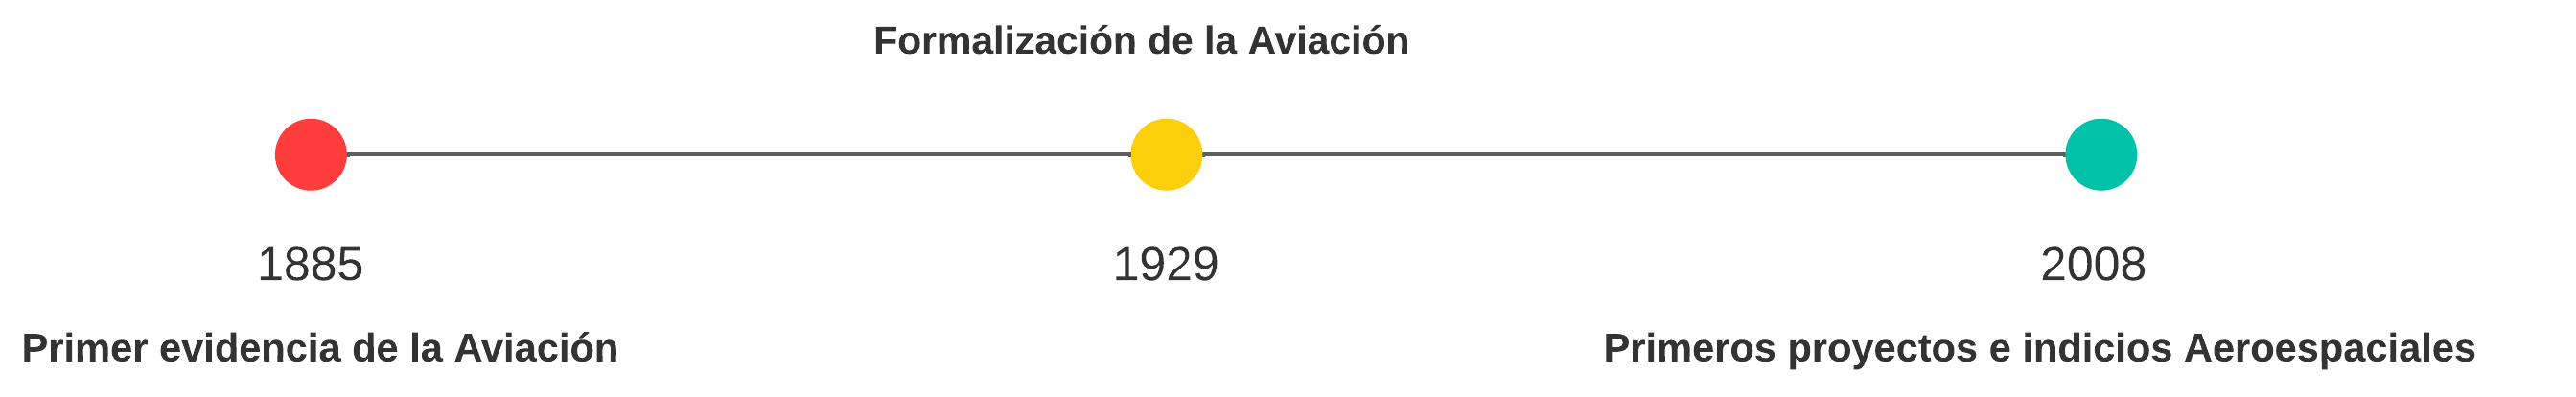
\includegraphics[width=0.85\linewidth]{document/figures/01_linea del tiempo_historia.png}
    \caption{Línea de tiempo de El Salvador, aviación y aeroespacial}
    \label{fig:historia}
\end{figure}

\newpage

\section{Objetivos} \label{sct:intro:objetivos}

\vspace{1.0cm}

\textbf{General}

Desarrollar un modelo de simulación de trayectoria ascendente y descendente de una globo-sonda hasta la estratosfera a través de la selección de diferentes parámetros clave para la misión aeroespacial.

\vspace{1.5cm}

\textbf{Específicos}

\begin{itemize}

    \item[•] Emplear los parámetros simulación que afectan la trayectoria ascendente y descendente de un globo-sonda en la estratosfera, y establecer los parámetros claves que delimiten la simulación.

    \item[•] Simular computacionalmente parámetros clave de un globo-sonda de gran altitud a lo largo de su posible trayectoria, de forma emulen las condiciones.

    \item[•] Desarrollar un análisis exploratorio a partir de los datos que se generaron en la simulación para proporcionar una visión general del equipo necesario para el subsistema de navegación en la misión estratosférica.

    \item[•] Elaborar un dimensionamiento a subsistema de navegación que consista en la selección de componentes electrónicos basándose en el análisis exploratorio realizado, culminando en el desarrollo de esquemático y layout para generar los archivos planteen una futura fabricación.

\end{itemize}

\newpage

\section{Aspectos a considerar} \label{sct:intro:consideraciones}

\subsection{Alcances}

\begin{itemize}

    \item[•] Se plantea el desarrollo de un código fuente capaz de simular la trayectoria dentro de la misión que imiten las condiciones posibles de la misión aeroespacial en la estratosfera, así como la generación de datos de simulaciones para elaborar un análisis exploratorio. 

    \item[•] Proponer un dimensionamiento a subsistema de navegación de bajo costo que incluya los dispositivos necesarios para rastreo de trayectoria y que sean aptos para las condiciones adversas y extremas de la estratosfera basándose en el análisis exploratorio realizado con los datos generados de la simulación.

    \item[•] Proporcionar como producto de este trabajo una herramienta útil para el diseño y la planificación de misiones aeroespaciales similares en el futuro. Ver anexo \ref{chp:anexo:source_thesis}.


\end{itemize} 

\subsection{Limitaciones}

\begin{itemize}

    \item[•] Ningún modelo puede simular y predecir con exactitud y además involucrar todos los parámetros existentes, esto debido a la gran variabilidad de los factores que se pueden encontrarse a lo largo de la trayectoria estratosférica del globo-sonda.

    \item[•] La propuesta de dimensionamiento a subsistema de navegación sólo incluye el desarrollo del esquemático y layout de los circuitos, y también los archivos para una futura fabricación, por lo tanto, excluye la realización de la programación y elaboración en físico de la placa de circuito impreso (PCB). Además, por lo último mencionado, no se realizan pruebas de funcionamiento ni pruebas de exposición de la PCB a las condiciones que emulen los parámetros de las simulaciones del código fuente a realizar.

    \item[•] La selección de componentes en el dimensionamiento del subsistema de navegación está limitada por los recursos disponibles, el alcance y precisión de los sensores; así como también, la disponibilidad y accesibilidad de los componentes electrónicos en el mercado internacional y local.

\end{itemize}

\newpage

\section{Motivación del trabajo} \label{sct:intro:motivacion}

El desarrollo de misiones aeroespaciales como lo serían las estratosféricas plantea un gran desafío, debido a la complejidad de los factores atmosféricos que afectan la trayectoria ascendente y descendente de un globo-sonda, así como los cambios meteorológicos que se presentan a diferentes altitudes que son extremos y cambiantes; es por ello, que es necesario tener una comprensión de las condiciones que se estarán expuestos y realizar simulaciones que modelen una aproximación de las circunstancias posibles de la misión aeroespacial. Con anterioridad, en El Salvador se han desarrollado globos estratosféricos de forma aficionada o en círculos académicos/profesionales \cite{globo_pupuseriasuiza_1},  \cite{globo_nayib_nuevocuscatlan}, \cite{sphere_ESAI}, y existe una constante de hechos comunes que dificultaban el éxito de las misiones de las sondas desarrolladas por ellos, se pueden resaltar algunos: pérdida de equipo, incerteza total o parcial del funcionamiento de la sonda en todo su recorrido y desconocimiento del ambiente/condiciones que podría enfrentar la sonda.

Entonces, es así como este trabajo aborda estos desafíos, proporcionando una solución con el modelamiento de la sonda en su trayectoria para tener una mayor certeza del funcionamiento y situaciones que se enfrenta el equipo y así lograr disminuir costos por perdidas, mitigar riesgos y aumentar las probabilidades de éxito de la misión. Adicional al modelo, se dimensiona un subsistema de navegación que integre una variedad de dispositivos de bajo costo, los más adecuados para las condiciones extremas de la estratosfera y su rastreo/localización;  con el análisis exploratorio se  selecciona los componentes electrónicos y desarrollar el esquemático y layout, generando los archivos necesarios para futura fabricación.

La inspiración para el presente trabajo proviene del proyecto Sphere de ESAI USA y otros proyectos consultados \cite{ sphere_ESAI}, \cite{Irazu_CR}, \cite{pycubed}, ya que no existe ninguna publicación en la región de Centroamericana relacionada con globos meteorológicos o estratosféricos de forma académica, exceptuando usos o aplicaciones comerciales, recreativas y aficionadas documentados en diarios nacionales y publicaciones a lo largo de internet \cite{globo_pupuseriasuiza_1},  \cite{globo_nayib_nuevocuscatlan}, \cite{globo_pupuseriasuiza_2}. Por lo tanto, el presente representa una oportunidad única para explorar y avanzar en esta área de investigación en la región y contribuir a desarrollar subsistemas de navegación de bajo costo para futuras misiones a la estratosfera, así como será beneficioso para futuros investigadores que desean recopilar o procesar datos meteorológicos o con algún otro propósito científico.

\newpage

\section{Contexto del proyecto} \label{sct:intro:contexto}

\subsection{Antecedentes}

Este trabajo tiene sus raíces en el macroproyecto "Diseño de la misión para un globo meteorológico de gran altitud - StratoBalloon", el cual fue creado por el Observatorio Micro Macro (OMM) de la Universidad Don Bosco. Este macroproyecto surgió a partir de la participación de un grupo de estudiantes de ingeniería en el hackathon "Space Apps Challenge 2021" de la NASA \cite{SpaceApps_ASAUDB}, \cite{SpacaApps_noticia_UDB}, donde se logró destacar entre los cinco mejores competidores a nivel nacional. Desde entonces, el equipo ha estado trabajando, llevando a cabo diferentes trabajos de graduación y otras actividades relacionadas con el mismo; uno de los trabajos de graduación realizados hasta la fecha se tituló “Diseño y análisis de un módulo reemplazable para misiones cercanas a la estratosfera (Near-Space LRU)”, desarrollado por Ali Barahona y Manuel Pleites. Este proyecto se enfocó en la parte estructural del macroproyecto y consistió en la realización de impresiones 3D de probetas de ensayo para probar la resistencia mecánica de materiales de impresión, además de realizar diferentes simulaciones mecánicas \cite{tesis_estructura_stratoballoon}.

Se tiene, también que,  "Diseño de la misión para un globo meteorológico de gran altitud - StratoBalloon", es una iniciativa salvadoreña liderada principalmente por un equipo de estudiantes de la Universidad Don Bosco de diversas disciplinas que trabajan juntos para lograr el objetivo de diseñar una misión para un globo meteorológico que pueda ascender a una altitud de 30,000 metros sobre el nivel del mar, con esto se busca obtener una experiencia valiosa en cuanto a liderazgo, trabajo en equipo y habilidades técnicas. El proyecto implica una serie de actividades integradoras para lograr el objetivo que abarcan desde la selección de materiales y equipos necesarios para la misión, hasta el cálculo de trayectorias y la obtención de los permisos legales necesarios para llevar a cabo la misión. 

La misión prevista del macroproyecto abreviada StratoBalloon, ver figura \ref{fig:etapas_mision_stratoballoon},  se desglosa y detalla en las siguientes fases de operación:

\begin{itemize}
    \item \textbf{Fase 1:}  lanzamiento de la sonda desde unas coordenadas predefinidas.
    \item \textbf{Fase 2:} ascenso de la sonda hasta los 30 km.
    \item  \textbf{Fase 3:} explosión del globo, inicia descenso en caída libre.
    \item \textbf{Fase 4:} descenso junto con el paracaídas y la carga útil.
    \item \textbf{Fase 5:}  recuperación de la sonda, fin de la misión.
\end{itemize}

Además,  las fases se pueden dividir en tres: despegue, apogeo y aterrizaje, siendo una versión resumida de las cinco fases presentadas.

\newpage

\begin{figure} [!ht]
    \centering
    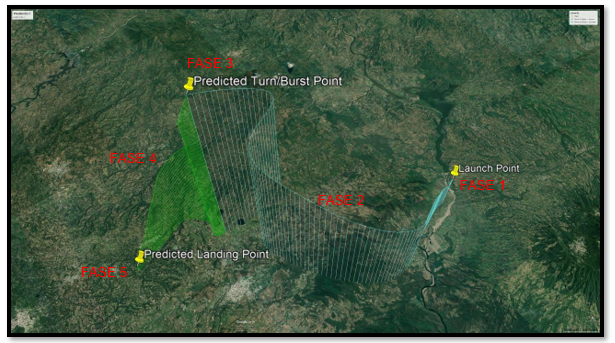
\includegraphics[width=1\linewidth]{document/figures/01_etapas de la mision.png}
    \caption{Etapas de la misión proyectada para StratoBalloon, créditos a \cite{tesis_estructura_stratoballoon}.}
    \label{fig:etapas_mision_stratoballoon}
\end{figure}

Cabe resaltar que en la fase 3 de la operación, véase figura \ref{fig:etapas_mision_stratoballoon}, es donde se alcanza el punto más crítico de la misión para los elementos electrónicos que componen el sistema, pudiendo alcanzar hasta los límites de la estratosfera, siendo afectado por temperaturas extremas, presión casi de vacío, nula densidad atmosférica, aumento de la radiación, humedad, entre otras \cite{nearspaceExperiments}.

En figura \ref{fig:bosquejo_stratoballoon} se muestra el bosque actual desarrollado en StratoBalloon, el cual es un prototipo que aún se está desarrollando y se le van haciendo mejoras a medida el proyecto avanza y se gana experiencia.  En donde se indica '\textit{módulo}' en la figura \ref{fig:bosquejo_stratoballoon},  es el diseño de la estructura actual, en cuyo interior existirán un conjunto de sistemas electrónicos que tienen el propósito de proveer la ubicación espacial, mantener comunicación con una estación en tierra y suministrar y administra la potencia eléctrica entre los demás subsistemas (navegación, telemetría y energía). 


\begin{figure} [!ht]
    \centering
    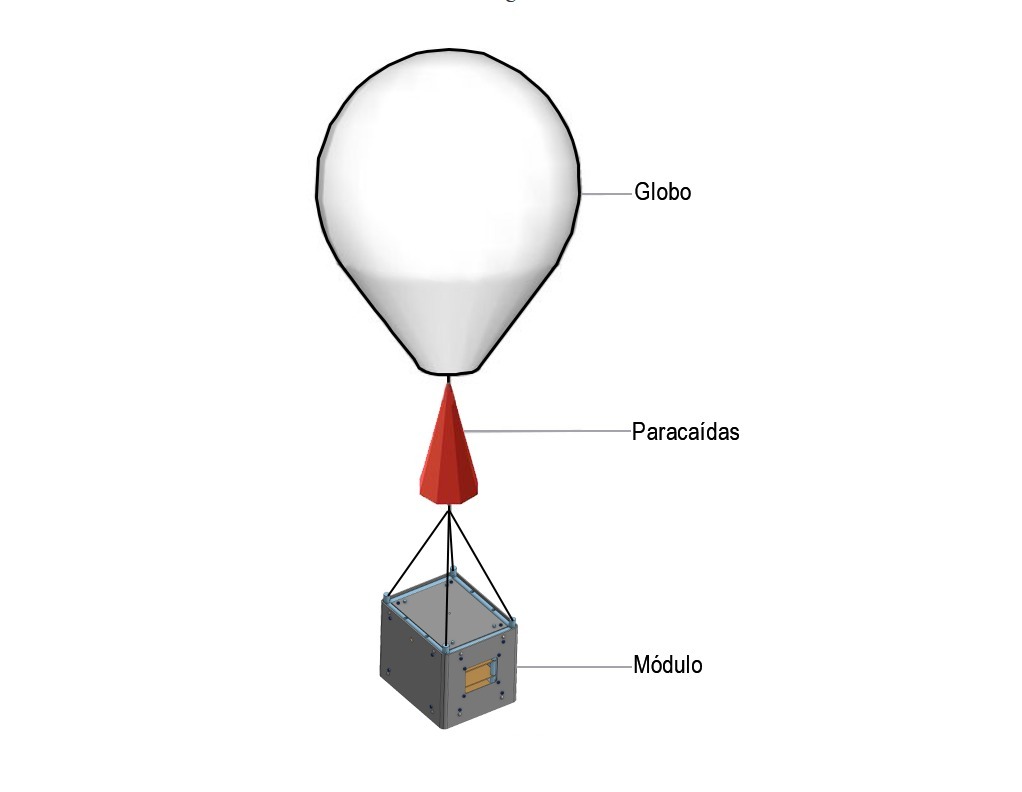
\includegraphics [width = 0.75\textwidth] {document/figures/01_componentes del globo}
    \caption{Bosquejo de StratoBalloon, créditos a \cite{tesis_estructura_stratoballoon}.}
    \label{fig:bosquejo_stratoballoon}
\end{figure}

\newpage

\subsection{Precedentes}

En el campo de la exploración espacial, en la última década se han desarrollado diversas plataformas open-source que han facilitado el  acceso y  democratizado la tecnología espacial como: 
 \begin{itemize}
     \item ArudPilot \footnote{ArduPilot Website: \url{https://ardupilot.org/}}.
     \item Dronecode \footnote{Dronecode foundation Website: \url{https://www.dronecode.org/}}
     \item Pycubed \footnote{Pycubed website: \url{https://pycubed.org/}}
     \item HabHub \footnote{HabHub website: \url{https://habhub.org/}}
 \end{itemize}

Las plataformas anteriormente listadas,  se ven principalmente impactadas en espacios académicos o por aficionados interesados en la exploración espacial, lo que contribuye a su crecimiento constante día a día. Existen y se pueden encontrar otras plataformas o precedentes a lo largo de internet, sin embargo, las plataformas que se mencionan a continuación  en subsubsecciones \ref{ssct:intro:pycuebed} y \ref{ssct:intro:habhub} han impactado significativamente el presente trabajo.

\newpage

\subsubsection{PyCubed} \label{ssct:intro:pycuebed}

Es un proyecto que desarrolla software y hardware en Python para  nanosatélites en estándar CubeSat, es apoyada por la Universidad de Stanford y dentro de sus recursos digitales se pueden encontrar las publicaciones realizadas, el código fuente, los diseños de las PCB's y diferentes misiones realizados con la iniciativa de este trabajo. Esta información  está habilitada en GitHub \footnote{Repositorio online: \url{https://github.com/pycubed}} o en su página web \footnote{Página Web: \url{https://pycubed.org/} }. 

La plataforma PyCubed, toma como ventaja que la electrónica embebida sigue en auge y en la última década ha existido una explosión importante, haciendo que el hardware se integra cada vez más y se utiliza ampliamente en todas las disciplinas de la ingeniería.  Esto se puede ver reflejado en las misiones KickSat-2 \cite{pycubed_kicksat-2}  y V-R3x \cite{pycubed_v-r3x} siendo avalados según sus propósitos de investigación por NASA.

En figura \ref{fig:ejemplo_pycubed}, se muestra una placa con características de bajo costo y la funcionalidad de integrar varios subsistemas (telemetría, navegación, energía, etc.) en una sola placa de circuito impreso.

\begin{figure}[!ht]
    \centering
    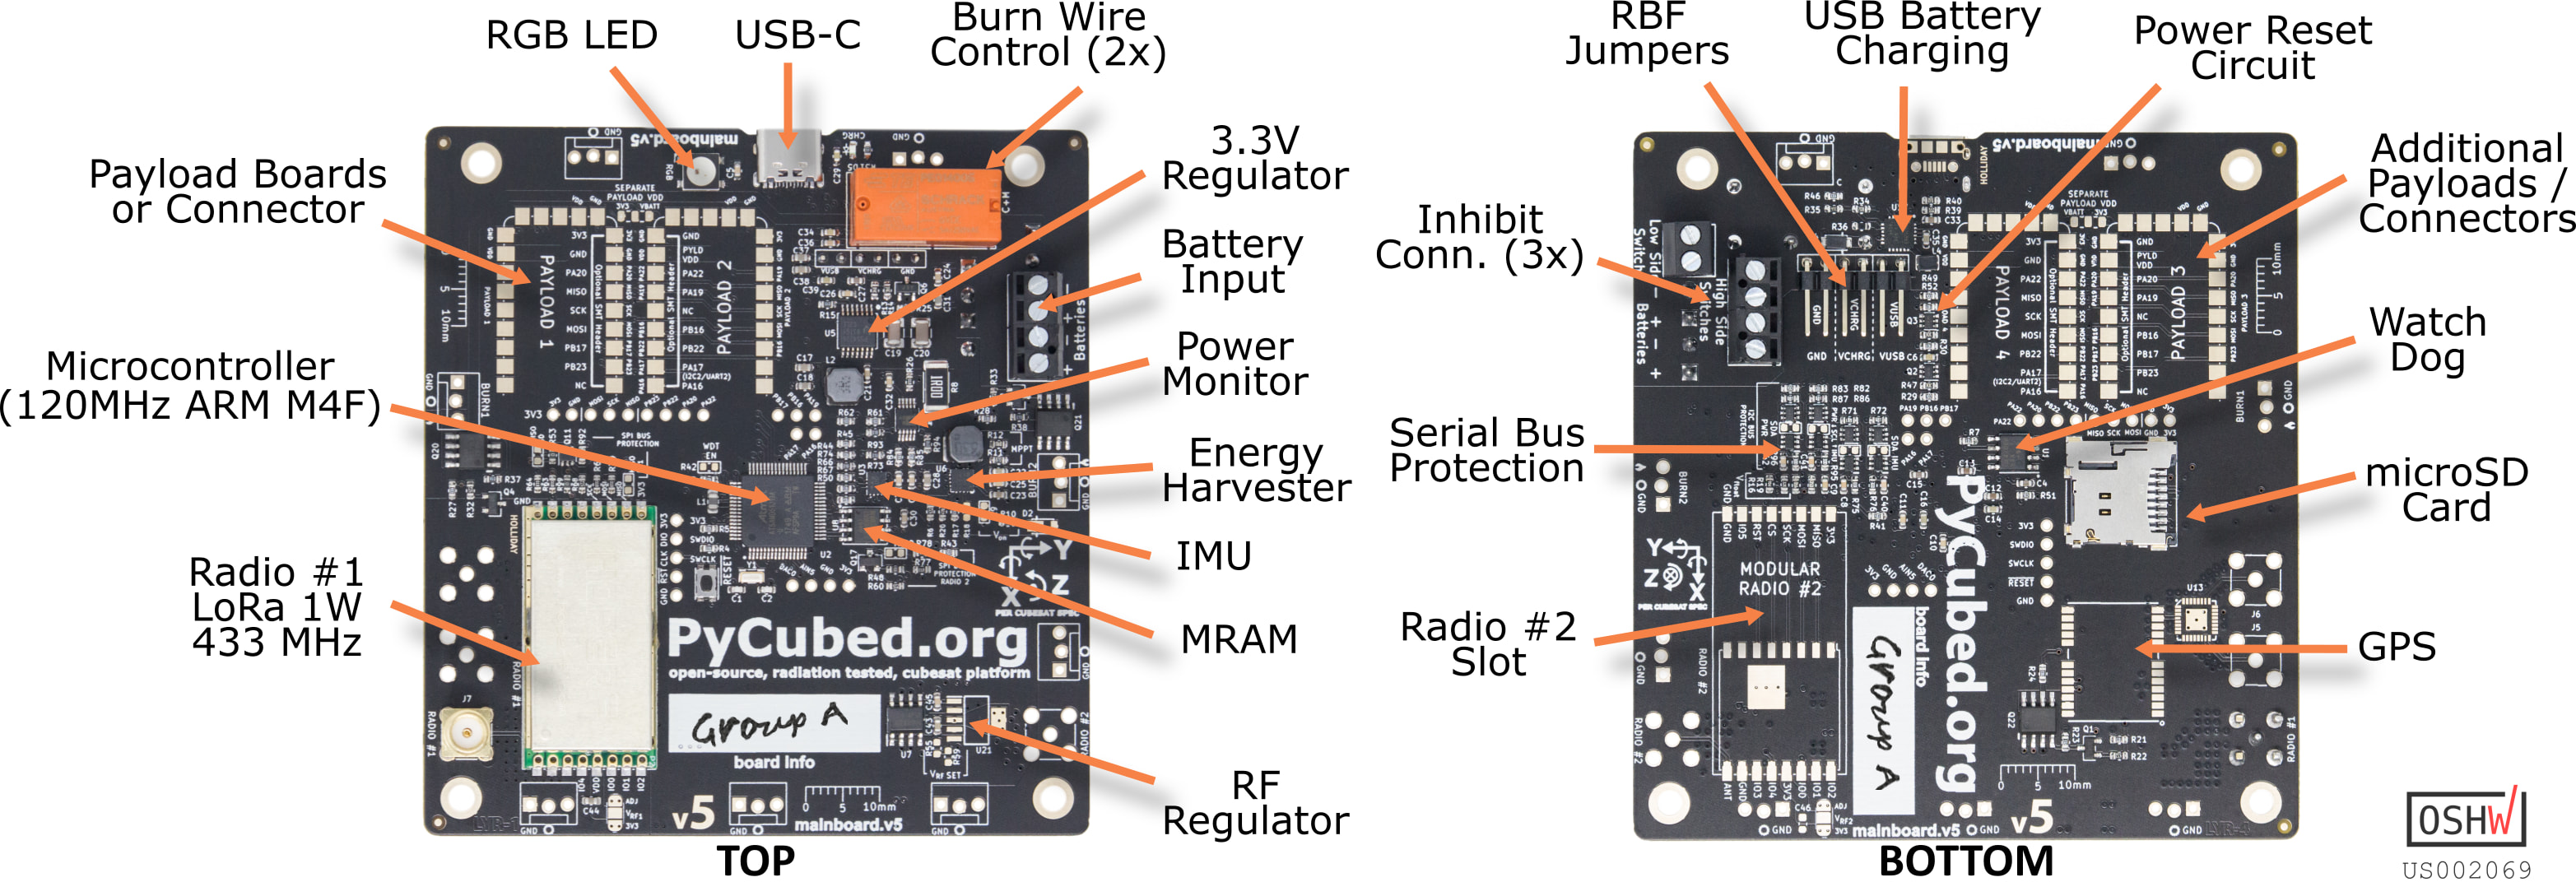
\includegraphics[width=0.75\linewidth]{document/figures/01_pycubed_ejemplo.jpg}
    \caption{PCB realizado por PyCubed, tomada de GitHub bajo CC BY-SA 4.0, sin modificación.}
    \label{fig:ejemplo_pycubed}
\end{figure}

\subsubsection{Habhub} \label{ssct:intro:habhub}

Es una plataforma dirigida por UK High Altitude Society (UKHAS)  que poseen múltiples herramientas en lo relacionado con globos de gran altitud, las cuales incluye: seguimiento y almacenamiento de los datos de vuelo, predicción de trayectoria y calculadora de explosión según la altitud. Además, incluye documentación y guías para montar un globo de forma aficionada\footnote{Página web:  \url{https://habhub.org/}}, ver figura \ref{fig:habhub}. 

\newpage

\begin{figure}[!ht]
    \centering
    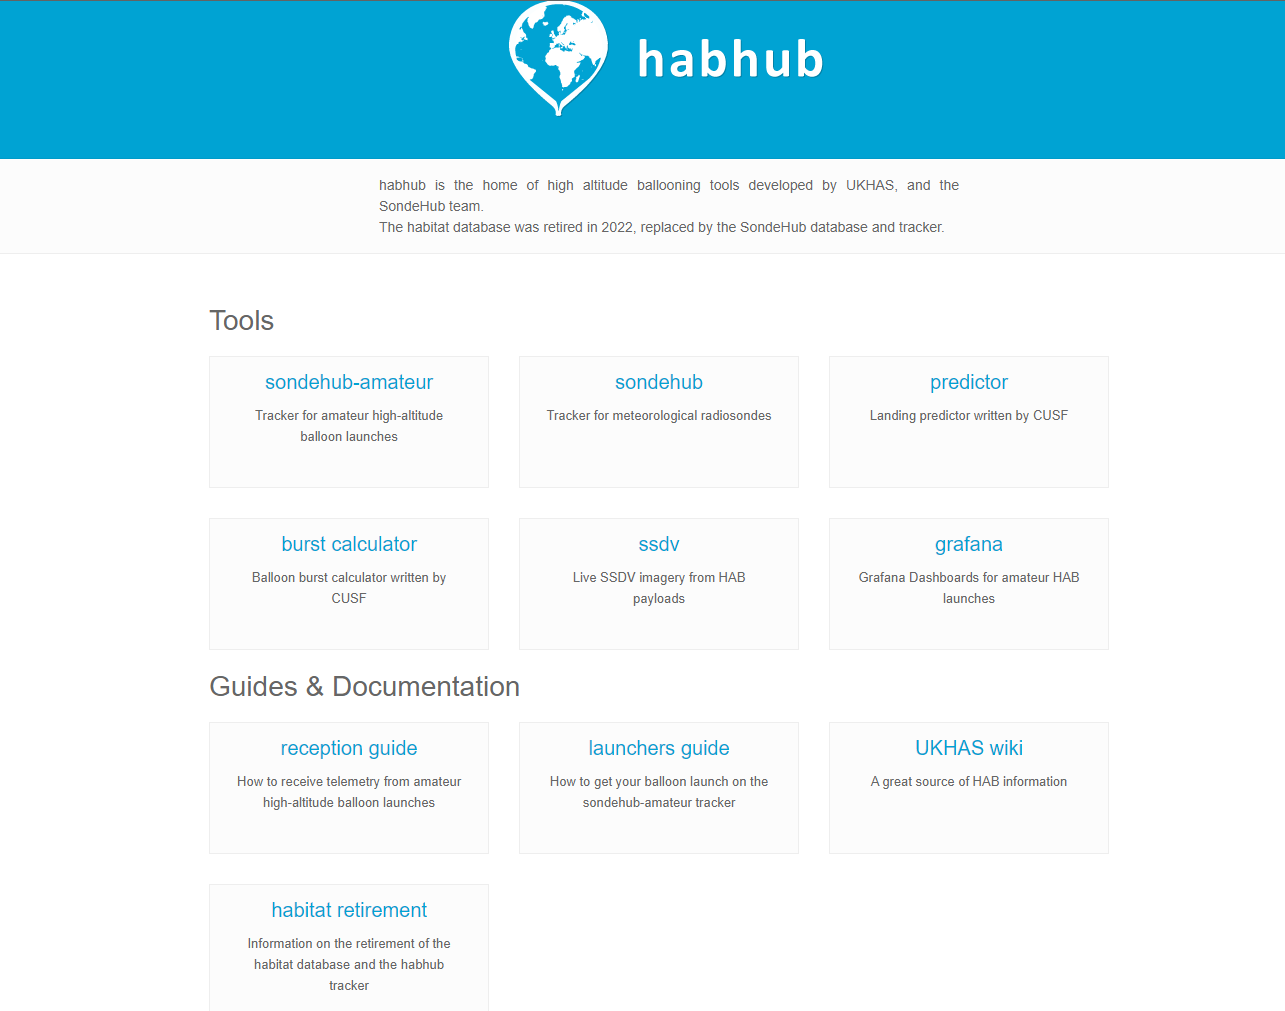
\includegraphics[width=0.5\linewidth]{document/figures/01_habhub_inicio.png}
    \caption{Inicio de la página web de habhub}
    \label{fig:habhub}
\end{figure}

Al visitar la página de HabHub y explorar las diferentes herramientas que ofrece (ver figura \ref{fig:cal_predic_habhub}), se encontró una calculadora útil para determinar la altitud de explosión de un globo de gran altitud. Esta calculadora recibe como parámetros de entrada el peso del payload, el tipo de globo, el objetivo de altitud o el objetivo de tasa de ascenso, y luego calcula la cantidad de gas de elevación (por defecto, se utiliza helio). Además, se encontró un software de predicción de ruta desarrollado por CUSF (Cambridge University Spaceflight) que acepta como parámetros la fecha, el lugar de lanzamiento, la altitud objetivo, entre otros (ver Figura \ref{fig:cal_predic_habhub}). El código fuente de la calculadora se puede consultar en internet\footnote{Calculadora: \url{https://github.com/projecthorus/cusf-burst-calc}} y el del software de predicción en\footnote{Software de predicción: \url{https://github.com/projecthorus/leaflet_predictor}}.

\begin{figure}[!ht]
    \centering
    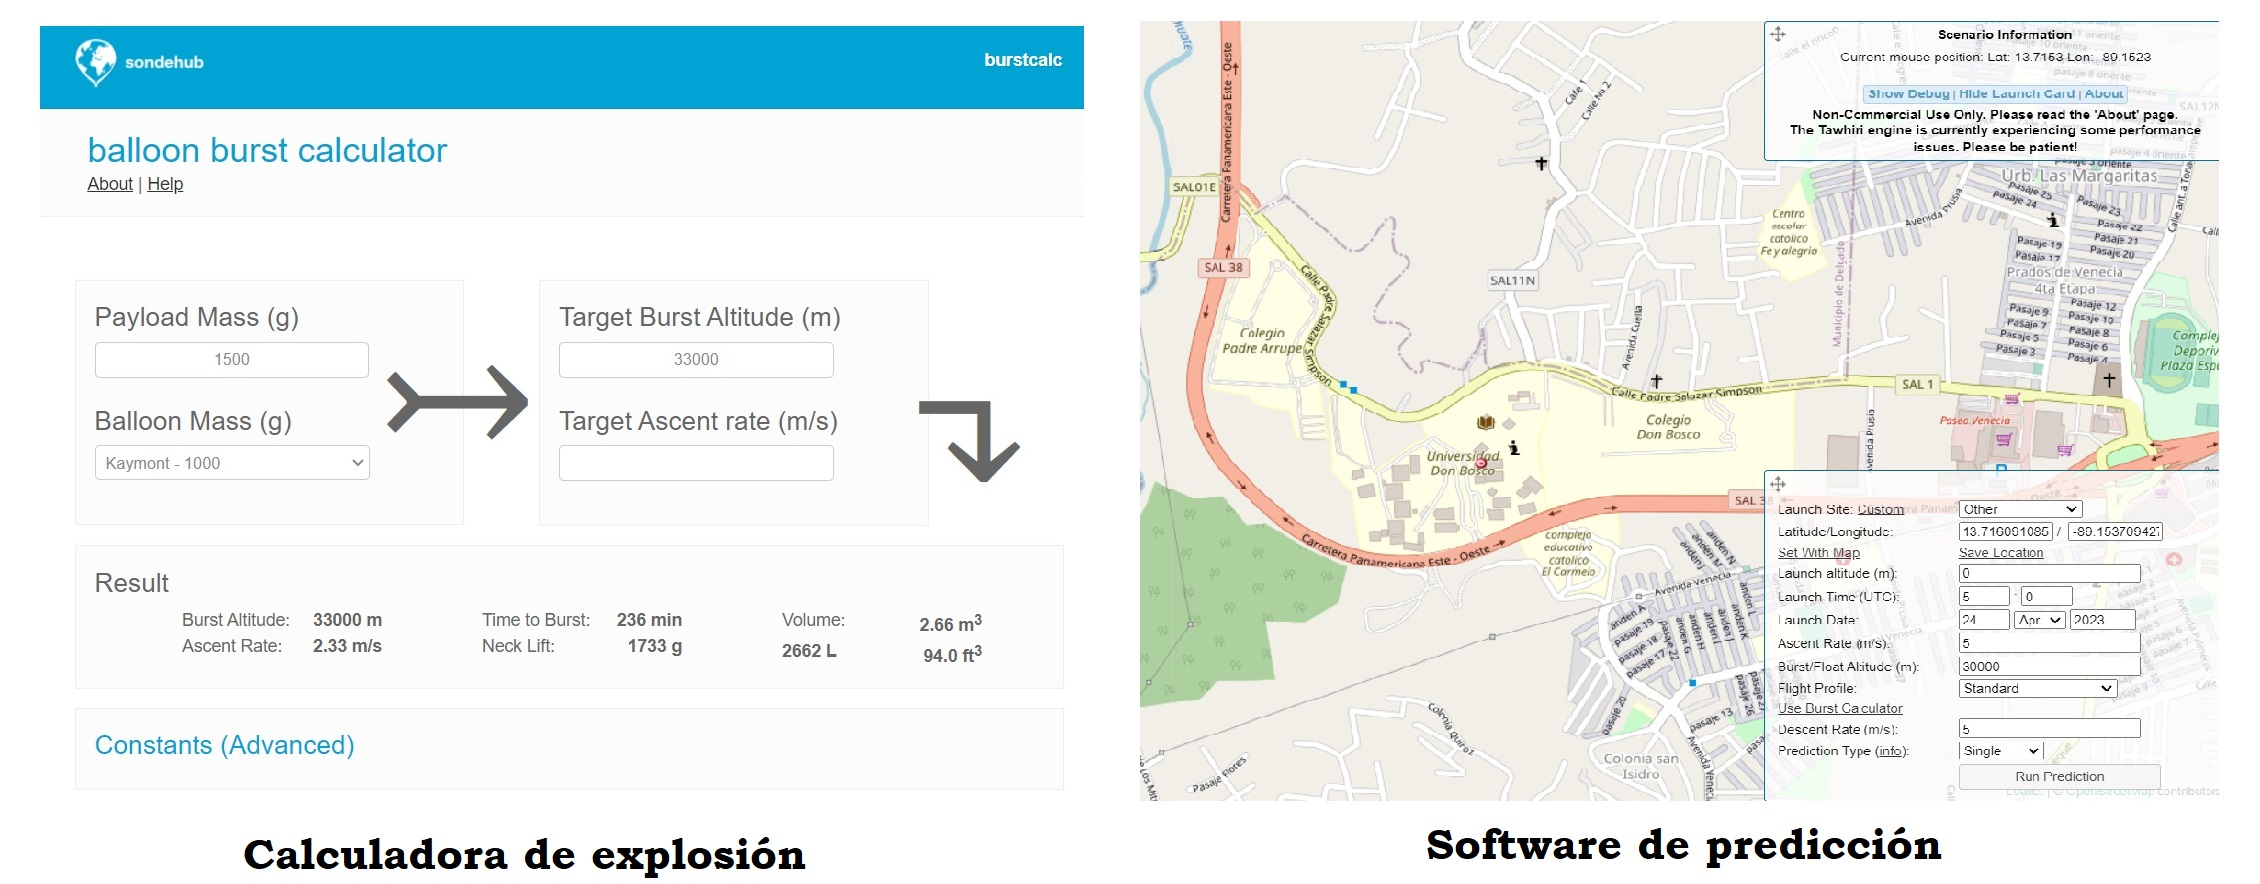
\includegraphics[width=0.95\linewidth]{document/figures/01_predic_calcBurst_habhub.jpg}
    \caption{Herramientas en su website, HabHub}
    \label{fig:cal_predic_habhub}
\end{figure}

\newpage

\subsection{Generalidades de los globos}

En lo que se refiere a la historia, ver figura \ref{fig:historia_globos},  se tiene registro del uso de globos en desde el siglo III en China se usaban como juguetes, fue hasta 1783 que los hermanos Montgolfier llenaron un globo de aire caliente llevando una persona en la ciudad París, Francia, los cuales ahora son llamados globos aerostáticos; y así fueron pasando los años se fueron realizando nuevos progresos haciendo que los globos lleguen más altos, se inventaron nuevos conceptos y tipos de globos hasta los de hoy en día \cite{history_type_balloon}.

\begin{figure}[!ht]
    \centering
    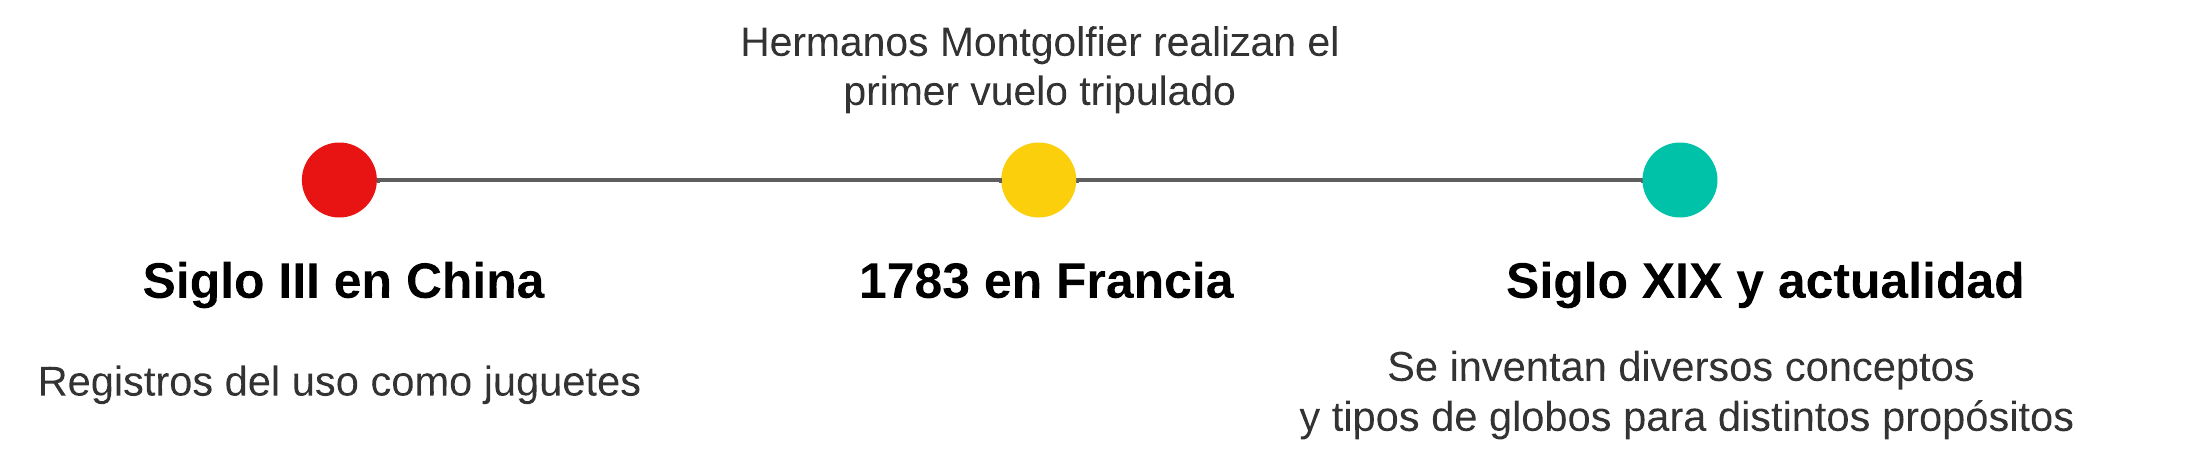
\includegraphics[width=0.5\linewidth]{document/figures/01_LineaTiempo_Globo_Historia.png}
    \caption{Evolución de los Globos a lo largo de la Historia}
    \label{fig:historia_globos}
\end{figure}

Los Globos de Gran Altitud (HAB), los cuales son vehículos semi espacial ligeros que transportan una carga y son capaces de sustentarse por medio de un gas como helio, nitrógeno, hidrógeno e incluso gas de carbón, ya que son menos densos que el aire. Estos vehículos obedecen al principio de Arquímedes en cuanto a la flotabilidad de un cuerpo y el peso aparente cuando están en otros fluidos, es decir, al diferenciar la densidad del vehículo con la densidad del aire y resulta que el peso aparente del vehículo es menor a cero, este será capaz de elevarse \cite{libro_fisica_giancoli}.

Un globo sonda está constituido generalmente por las siguientes componentes, que recuerda a figura \ref{fig:bosquejo_stratoballoon}:

\begin{itemize}
    \item \textbf{Globo:} Es la parte principal, el tipo de globo varía de acuerdo a la aplicación.
    \item \textbf{Paracaídas:} Una vez que el globo alcanza su altitud máxima, se hace necesario su descenso controlado y seguro para evitar daños en los equipos y garantizar la seguridad de las personas y propiedades en tierra.
    \item \textbf{Carga Útil:} Depende mucho del tipo de misión a realizar, sin embargo, algunos componentes comunes podrían ser: instrumentos científicos, sistema de comunicaciones y ubicación. 

\end{itemize}

\subsubsection{Tipos de Globos} \label{tipos_globo}

Los globos se pueden clasificar de muchas formas como podrían ser su aplicación, tipo de gas elevador, tripulados o no tripulados, uso civil, científico o militar, etc. Sin embargo, los globos sonda de gran altitud, los cuales son el interés para este trabajo,  se clasifican como indica \cite{type_balloon_NASA, history_type_balloon, just_type_balloon} de esta forma:  

\begin{itemize}
    \item \textbf{Sounding Balloon or Weather Balloon}: en español se conocen como globos meteorológicos, son típicamente fabricados en látex y son diseñados para expandirse y explotar a una altura determinada, recolectando datos en su ascenso, sin superar la estratosfera.  Existe una variedad de nombres tanto en inglés como en español para este tipo de globo, así como una diversidad de aplicaciones y usos según el contexto. Principalmente, se observa su uso en universidades y centros de investigación. 
    \item \textbf{Equal pressure or Zero-pressure Balloons}: Los globos aerostáticos de igual presión o presión cero transportan cargas útiles a grandes altitudes en la atmósfera terrestre. Se diferencian de los globos de gas convencionales en que se llenan de helio a temperatura ambiente y se dejan expandir de forma natural a medida que ascienden, en lugar de inflarlos con gas a presión. Al incorporar una bolsa de lastre o un sistema de válvulas que libera gas cuando la presión dentro del globo aumenta debido al ascenso de este, los globos mantienen su forma.
    \item \textbf{Super Pressure Balloons}: conocidos en español como "globos de superpresión" mantienen una altitud y una forma constantes al mantener una sobrepresión continua dentro de la envoltura del globo. Se utilizan para la investigación científica. Pueden transportar cargas más pesadas durante períodos más largos que otras variedades de globos aerostáticos porque no les afectan las variaciones de la presión atmosférica. Su tamaño y peso, que dificultan su lanzamiento y recuperación.
\end{itemize}

A continuación, se muestra en figura \ref{fig:type_balloons} los tipos de globos ordenados según se listaron anteriormente. Créditos a las imágenes a \footnote{NASA/Bill White. Ver en: \url{https://www.flickr.com/photos/nasakennedy/36612463502}} \footnote{NASA. Ver en: \url{https://www.flickr.com/photos/nasafo/48877773637}} \footnote{NASA/Bill R. En: \url{https://www.flickr.com/photos/nasakennedy/36612463502}}, tomadas de Flickr.

\begin{figure}[!ht]
    \centering
    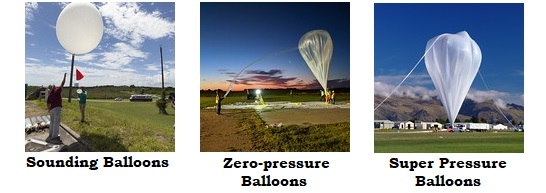
\includegraphics[width=0.9\linewidth]{document/figures/01_type_ballons.jpg}
    \caption{Tipo de globos de gran altitud}
    \label{fig:type_balloons}
\end{figure}


\chapter{Desarrollo de Simulación de Trayectoria} \label{chp:02_simulacion}

\vspace{0.2cm}

La simulación de trayectoria de un globo sonda es un recurso importante en investigaciones atmosféricas o aeroespaciales, como es el caso de este trabajo, estos simuladores permiten pronosticar y planificar el vuelo de globos, los cuales se basan en modelos matemáticos que describen el comportamiento del  espacio físico donde se desarrolla su trayecto.

\vspace{0.5cm}

En este capítulo se analizan tres modelos físicos matemáticos utilizados en la simulación de trayectoria: modelo atmosférico, modelo geométrico y  modelo dinámico. Cada uno de estos modelos tiene sus propias características y supuestos, que se describen en detalle de forma general y luego de forma específica, además, todos utilizan  el sistema internacional  de unidades.

\newpage

\section{Hipótesis de los modelos} \label{sct:simulacion:hipotesis}

Se describe de forma general los supuestos de la simulación en los diferentes modelos a utilizar; basándose en estos supuestos se identifican y delimita el simulador de trayectoria ascendente y descendente. 

\vspace{0.7cm}

A continuación, los supuestos:

\begin{enumerate}
    \item  El sistema obedece la ley de los gases ideales (ver
anexo \ref{chp:anexo:gases_ideales}), ecuación de la hidrostática (ver anexo \ref{chp:anexo:hidrostatica}) y leyes del movimiento de Newton (mecánica clásica) a lo largo de la trayectoria \cite{libro_dinamica_beer}. 
    \item No existe humedad, radiación solar en la hipotética distribución vertical estratosférica de la trayectoria \cite{isa_1976}. Además, en su distribución vertical la presión interna del globo y externa de la atmósfera se asumen iguales, así mismo la temperatura del globo y la atmósfera. 
    \item Se asume que el sistema emula una partícula de característica esférica con tres grados de libertad, siendo considerada una masa puntual donde interactúan todas las fuerzas que actúan sobre el sistema. Por lo tanto,  por ser un sistema de tres grados de libertad no existen momentos.
    \item  Las componentes horizontales de la velocidad del globo son iguales a las componentes horizontales de la velocidad del viento \cite{lsoda, simulador_chino}, es decir, $\vec{v}_{viento} = \vec{v}_{globo} $ .  Además, se utilizó la convención de meteorología de tener dos componentes de viento U y V, que según su convención la componente U del viento representa el flujo de viento de oeste a este positivo a lo largo de la latitud y la componente V del viento representa el flujo de viento de sur a norte positivo a lo largo de la longitud.
    \item Se toma como premisa que el día y hora del lanzamiento del globo sonda los vientos tiene un comportamiento típico en el proceso de descenso y ascenso. La simulación, en la fecha seleccionada, representa la trayectoria característica que cualquier globo sonda podría experimentar.
\end{enumerate}

\vspace{0.7cm}

La simulación forma parte de modelos estocásticas e hipotéticos de cómo funcionan la distribución vertical de las variables atmosféricas y meteorológicas. Además, no se consideran los modelos térmicos ni elásticos por deformación del globo debido a la duración y enfoque que estos tienen, a diferencias de los zero pressure balloon vistos en subsubsección \ref{tipos_globo} que si es necesario por el tiempo que pasan en la atmósfera que puede ser de unos días, semanas o incluso meses.


\newpage

\section{Datos de entrada e Inicio}

Para la implementación de este trabajo se requiere tener datos de las condiciones iniciales o componentes a utilizar previos a realizar la simulación. En las siguientes subsecciones se detalla esta información antes de  entrar de lleno con los modelos a utilizar.

\subsection{Componentes del Sistema}

La selección de los componentes que se añaden al sistema de globo sonda incluye el paracaídas y el globo mismo, la elección de estos componentes depende de la carga útil que se desea enviar en la misión. Para la simulación, se estima el peso de la carga útil (payload) basándose en el trabajo de graduación realizado por \cite{tesis_estructura_stratoballoon} sobre la estructura. La masa de la carga útil se calcula como 1.769 kg, con un volumen de 517.774 cm³.

Se llevó a cabo una búsqueda para encontrar un globo y un paracaídas comerciales que proporcionen la información requerida por el simulador. Los datos técnicos de estos elementos se muestran en la tabla \ref{tab:globo_datos} y \ref{tab:paracaidas_datos}, respectivamente en \footnote{\textbf{Datos del globo}: \url{https://www.kaymont.com/product-page/hab-1500}} \footnote{\textbf{Datos del paracaídas}: \url{https://the-rocketman.com/recovery-html/}}.

\vspace{0.7cm}
\begin{table}[h]
\centering
\begin{tabular}{ll}
\toprule
        \textbf{Parámetro Globo}                    & \textbf{Valor}  \\
\midrule
        Peso [kg]                  & 1.5    \\
        Diámetro de explosión [m]  & 9.44   \\
        Altitud máxima [m]   & 34,200 \\
        Presión crítica [hPa] & 6.3    \\
\bottomrule
\end{tabular}
\caption{Datos tomados de hoja técnica de Kaymont HAB-1500}
\label{tab:globo_datos}
\end{table}




\vspace{0.7cm}
\begin{table}[h]
\centering

\begin{tabular}{ll}
\toprule
\textbf{Paracaídas}                    & \textbf{Valor}  \\
\midrule
Peso [kg]                 & 0.0992    \\
Diámetro  [m]  & 1.56   \\
\bottomrule
\end{tabular}
\caption{Datos tomados de Rocketman 4ft High Altitude Balloon}
\label{tab:paracaidas_datos}
\end{table}

\newpage

\subsection{Condiciones iniciales y datos de entrada}

Las especificaciones  y la correspondiente información de datos de entrada o valores iniciales del sistema para la simulación de vuelo del globo sonda se presentan en la tabla \ref{tab:datos_start_input}. 

\begin{table}[h]
\centering
\caption{Especificaciones de globo-sonda e información de simulación de vuelo.}
\label{tab:datos_start_input}
\begin{tabular}{cc}
\toprule
              \textbf{Parámetros} &                  \textbf{Valor} \\
\midrule
Fecha y hora de Lanzamiento [UTC] &             2023-06-10 10:00:00 \\
         Objetivo de Altitud  [m] &                           30000 \\
              Base de lanzamiento & Lat: 13.808825, Lon: -89.328988 \\
        Altitud inicial [msnm]    &                             504 \\
                  Masa Globo [kg] &                            1.50 \\
                  Masa Helio [kg] &               0.568913691920873 \\
                Masa Payload [kg] &                            1.77 \\
             Presión Inicial [Pa] &                          101325 \\
          Temperatura Inicial [K] &                          288.15 \\
\bottomrule
\end{tabular}
\end{table}


Es relevante mencionar que el sistema globo sonda parte del reposo cuando es liberado, por lo tanto, su velocidad vertical es cero, solamente siendo afectado por velocidades horizontales por el viento. Además, la fecha y hora elegida no obedece ningún criterio, se hizo de forma arbitraria, pero se asume que se obtiene un comportamiento típico a comparación de otras fechas y horas de lanzamiento.

\subsubsection{Estimación del gas de elevación} \label{ssct:simulacion:gas_y_peso}

La cantidad del gas de elevación es fundamental en la simulación de trayectoria de un globo sonda, ya que permite  obtener la fuerza de empuje que eleva a  la carga útil (payload) y determinar la masa o volumen del gas necesario para llegar a la altitud objetivo o propósito de la misión aeroespacial.  Para desarrollar el cálculo su pudo utilizar dinámica o también aerodinámica con teorías de fluidos, sin embargo, con la intención de reducir la complejidad,  se optó por utilizar  el principio de Arquímedes, la ley de los gases ideales (ver anexo \ref{chp:anexo:gases_ideales}) e hidrostática (ver anexo \ref{chp:anexo:hidrostatica}), modelo estándar atmosférico que se explica más adelante en la sección \ref{sct:simulacion:modelo_atmoferico}  y modelo geométrico que también más se explica posteriormente en la sección \ref{sct:simulacion:modelo_geometrico}. Mayor información de los conceptos que aplican en la estimación según este trabajo en \cite{libro_fisica_giancoli, isa_1976}. 

\newpage

Con respecto a este trabajo, se utiliza el gas helio como gas de elevación\footnote{Existen muchos gases de elevación, los ideales son Hidrógeno y Helio. Lo que los hace gases de elevación es la diferencia de densidad respecto al aire, que es menor. Se prefiere Helio debido a que es más seguro su manejo y es un gas inerte.},  una vez seleccionado el gas se partió de la ecuación de los gases ideales (ver anexo \ref{chp:anexo:gases_ideales})  haciendo una comparación de un estado inicial del gas a un estado final  en el cual existe conservación de masa lo cual es algo lógico porque la masa del gas es constante en todo la trayectoria hasta la explosión del globo en la altitud objetivo asumiendo que no existan fugas del mismo, véase tabla \ref{tab:datos_start_input} altitud objetivo.  Con la anterior comparación del gas en sus estados final e inicial se tiene entonces la ley de los gases de esta forma: 


\begin{equation}
    \label{eq:masa_helio}
    \frac{P_{1} V_{1}}{ T_{1} } = \frac{P_{2} V_{2}}{ T_{2} }
\end{equation}


Donde en ecuación \ref{eq:masa_helio}, el subíndice 1 significa estado del gas en el punto de lanzamiento, punto 1; y subíndice 2 como el punto final al cual la sonda debe de alcanzar, punto 2. En ambos subíndices se conocen el valor de las variables del gas de ecuación \ref{eq:masa_helio} por el estándar  atmosférico \cite{isa_1976}

\textbf{En el punto 1} se conoce la presión y temperatura ($P_{1}$ y $T_{1}$), se desea conocer el volumen inicial o volumen de llenado del globo ($V_{1}$).

\textbf{En el punto 2} conocemos la presión, volumen y temperatura final ($P_{2}$, $V_{2}$ y $T_{2}$ respectivamente), además se toma en cuenta lo expuesto por la hoja técnica que puede soportar el globo seleccionado, ver tabla \ref{tab:paracaidas_datos}. 

Una vez calculada volumen inicial ($V_{1}$) se debe de despejar de la ecuación de la ley de los gases ideales ($PV = nRT$) para calcular la masa, además al resolver todo lo anterior explicado se pudo obtener el volumen inicial y diámetro inicial del globo como también su masa de llenado de helio. En el código de Python desarrollado se utilizó el módulo sympy\footnote{Más información de sympy: \url{https://www.sympy.org/en/index.html}} para resolver las diferentes ecuaciones. 

\textbf{Soluciones alternativas}

Existe otras formas de calcular la cantidad de Helio o gas de elevación utiliza, por ejemplo  en \cite{spain_simulador} se calcula primero el radio de lanzamiento del globo y  luego se obtiene el volumen, para por último hacer una formulación de la ecuación de ley de los gases ideales y obtener la masa del helio además de una comparación si existe flotabilidad. Además, se puede calcular usando dinámica \cite{libro_dinamica_beer},  dimensionando la fuerza de arrastre y fuerza de empuje, teniendo el sistema en reposo donde $\sum F = 0$  como lo indica \cite{lsoda, helio_estimatcion} . Se prefirió la forma mostrada en ecuación \ref{eq:masa_helio} debido a que así se tiene control de la altura objetivo a la cual se desea enviar y se reduce complejidad en el cálculo. 

\newpage

\section{Sistema de Coordenadas}

En figura \ref{fig:crs} se muestran la relación que pueden existir entre diferentes sistemas de coordenadas\footnote{ \href{https://commons.wikimedia.org/wiki/File:International_Standard_Atmosphere.svg}{ CC BY-SA 4.0, autor: Chuckage.  Shows the ECEF coordinates (x, y, z) of a point on the surface of a spheroid.} Sin modificación }. En este caso un cartesiano con un elipsoide de referencia y uno de coordenadas esféricas, los cuales pueden expresar el comportamiento de cualquier sistema que se desplace en el planeta tierra.

\begin{figure}[h]
    \centering
    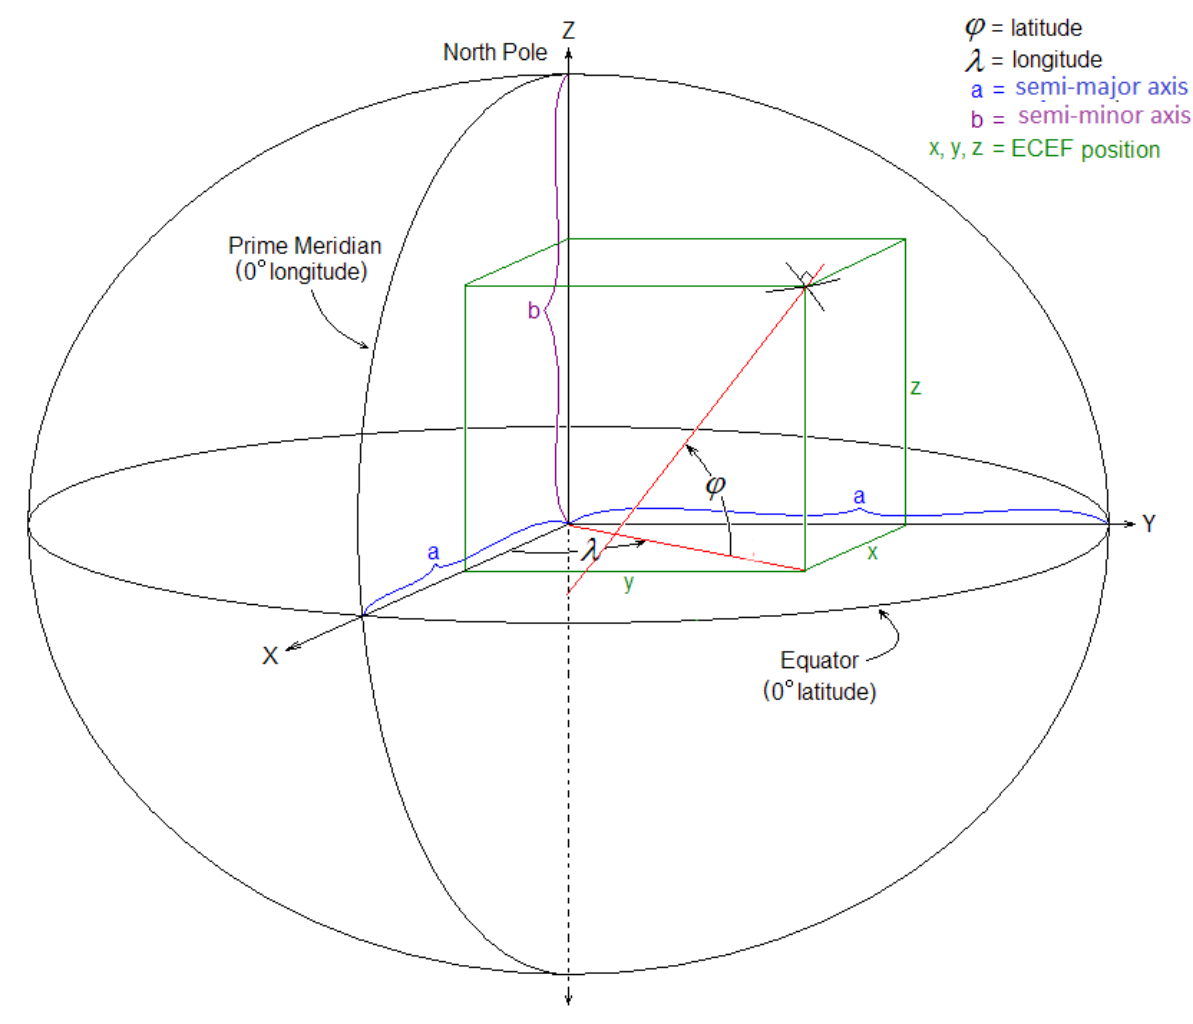
\includegraphics[scale=0.25]{document/figures/02_ECEF_coordinates.png}
    \caption{Sistema de coordenadas}
    \label{fig:crs}
\end{figure}
Por otro lado, en la simulación a desarrollar el movimiento espacial se ha caracterizado en  dos tipos:  vertical y horizontal. Dado el carácter que las distancias son cortas, la curva tierra no es apreciable, así que en su área de operación del globo sonda se trabaja como dos ambientes separados en el cual la vertical se moverá siguiendo la altitud en la que se encuentre en la tierra; por otro lado, en la horizontal, se analiza el problema como proyecciones de EPSG:4326 debido a que son las forma en que entrega la información los GPS en latitud y longitud (WGS84) \cite{libro_gnss},  y por otro lado, EPSG:3857 debido a que es la presentación renderizada de mapas como Google Maps \cite{google_maps}, OpenStreetMap, etc. La decisión está determinada por usar EPSG:4326 y EPSG:3857 para respectivamente tener grados y en la otra proyección usar metros así como están planteadas las ecuaciones diferenciales \ref{eq:viento_x} y \ref{eq:viento_y}, también esta decisión permite el uso de mapas.
 
\newpage

\section{Modelo Atmosférico} \label{sct:simulacion:modelo_atmoferico} 

Se utiliza la  ISA (International Standard Atmosphere) de 1976 \cite{isa_1976} para predecir las condiciones atmosféricas a diferentes altitudes, este modelo proporciona una referencia estándar, invariante e hipotética de la distribución vertical de la temperatura, presión y densidad en función de las diferentes capas de la atmósfera en todo el mundo.  

Además, se incluye información sobre la gravedad que son factores importantes en la trayectoria del globo sonda hasta altitudes estratosféricas. En figura \ref{fig:generalidad_ISA} \footnote{ \href{https://commons.wikimedia.org/wiki/File:International_Standard_Atmosphere.svg}{CC BY-SA 3.0, autor: Cmglee. Derivado de Comparison International Standard Atmosphere space diving.svg.} Sin modificación} se muestra una idea general de la distribución vertical según las diferentes capas de la atmósfera.

\begin{figure}[h]
    \centering
    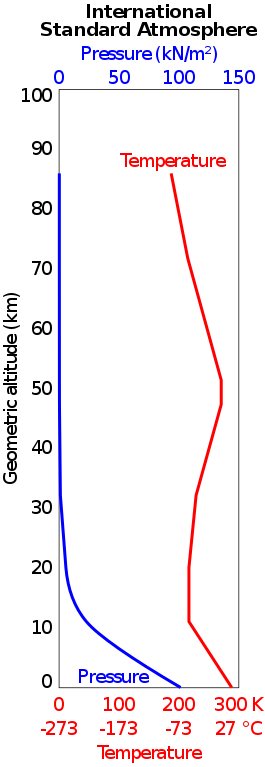
\includegraphics[scale=0.45]{document/figures/02_International_Standard_Atmosphere.png}
    \caption{Comportamiento de las variables  atmosféricas, temperatura y presión en las diferentes capas según ISA.}
    \label{fig:generalidad_ISA}
\end{figure}


\subsection{Gravedad}

La gravedad se hace más débil a medida que se aleja de la masa terrestre, es decir, no es constante a medida que se asciende, sino que disminuye en función de la altitud; esta formulación es proveída por la Ley del Inverso cuadrado  \cite{isa_1976}. Esta disminución se puede expresar de:

\begin{equation}
    \label{eq:gravedad}
    g = g_0 \left(\frac{R_e}{R_e + Z}\right)^2
\end{equation}

\textbf{Donde:}
\begin{itemize}
    \item 	$g_{0}$ es la aceleración estándar debida a la gravedad sobre el nivel del mar, con un valor de $ 9.80665 $  $ m/s^{2} $.
    \item 	$R_e$ es el radio promedio de la Tierra, con un valor de 6,371,000 m.
    \item 	$Z$ es la altitud sobre la superficie de la Tierra.
\end{itemize}

\subsection{Temperatura, presión y densidad} \label{ssct:simulacion:ISA_variables}

Debido a la naturaleza de los globos sonda se presenta un resumen de las capas estratosféricas a las cuales en su trayectoria se podría mover el globo sonda, en tabla \ref{tab:constantes_ISA}  y  \ref{tab:formulas_ISA}  se exponen respectivamente las constantes y ecuaciones matemáticas de las variables temperatura, presión y densidad del modelo atmosférico \cite{tabla_isa}.

% Tabla de las Constantes  ISA (temperatura, presión y densidad).
\begin{table}[ht]
\centering
\begin{tabular}{ccccc}
\hline
\textbf{Capa} & \textbf{$z_0$ [m]} & \textbf{$T_0$ [K]} & \textbf{$\lambda_0$ [K/m]} & \textbf{$P_0$ [Pa]} \\
\hline
1 & 0 & 288.15 & -0.0065 & 101,325.00 \\
2 & 11,019 & 216.65 & - & 22,632.10 \\
3 & 20,063 & 216.65 & 0.0010 & 5,474.89 \\
4 & 32,162 & 228.65 & 0.0028 & 868.02 \\
5 & 47,359 & 270.65 & - & 110.91 \\
\hline
\end{tabular}
\caption{Constantes de la ISA}
\label{tab:constantes_ISA}
\end{table}

% Tabla de las Ecuaciones ISA (temperatura, presión y densidad).

\begin{table}[ht]
\centering

\begin{tabular}{cccc}
\hline
\textbf{Capa} & \textbf{Temperatura [K]} & \textbf{Presión [Pa]} & \textbf{Densidad [kg/m$^3$]} \\
\hline
1 & $T_0 + \lambda_0 (z - z_0)$ & $P_0 \; \left( \frac{T_0}{T} \right)^{g(z) M_{air} / (R_{s} \lambda_0)}$ & $ P / (T \; R_{s})$ \\
2 & $T_0$ & $P_0 \; e^{-g(z) M_{air} (z - z_0) / (R_{s} T)}$ & $ P / (T \; R_{s})$ \\
3 & $T_0 + \lambda_0 (z - z_0)$ & $P_0 \; \left( \frac{T_0}{T} \right)^{g(z) M_{air} / (R_{s} \lambda_0)}$ & $ P / (T \; R_{s})$ \\
4 & $T_0 + \lambda_0 (z - z_0)$ & $P_0 \; \left( \frac{T_0}{T} \right)^{g(z) M_{air} / (R_{s} \lambda_0)}$ & $ P / (T \; R_{s})$ \\
5 & $T_0$ & $P_0 \; e^{-g(z) M_{air} (z - z_0) / (R_{s} T)}$ & $ P / (T \; R_{s})$ \\
\hline
\end{tabular}
\caption{Fórmulas de la ISA}
\label{tab:formulas_ISA}
\end{table}


\newpage

\section{Modelo Geométrico} \label{sct:simulacion:modelo_geometrico}

A medida el globo sonda asciende, el aire se volverá menos denso y el gas en su interior se expandirá por tal motivo, lo que provocará que la geometría del globo cambien,  para calcular tal fenómeno se aplica la Ley de los Gases ideales, la ISA y geometría. Entonces,  con lo anterior y dejando la ecuación en función de la altitud, se tiene:


\begin{equation}
    \label{eq:geometria}
    P(z) \; V = n \; R \; T(z) 
\end{equation}


Donde $ P(z) $ es la presión interna del gas, que será igual a la presión externa atmosférica;  $ n $ es la cantidad de moles del gas de elevación (helio) y $ T(z) $ la temperatura atmosférica igual que la temperatura del gas, por último $ R $ es la constante de los gases ideales.  Se ha asumido que el globo tiene forma esférica,  se  tiene que $r(z)$ como indica\cite{ascentRate_weatherBallon} es:

\begin{equation}
    \label{eq:radio}
    r(z) = \sqrt[3]{\frac{ 3 \; m \; R \; T }{ 4 \pi \; P \; M }}   
\end{equation}
 
La ecuación \ref{eq:radio} se utiliza para determinar tanto en área como en volumen del globo, como se indica en los siguientes apartados. Como dato de entrada para aplicar esta ecuación, es necesario conocer la masa del helio con la cual fue llenado el globo sonda como se indicó en subsubsección \ref{ssct:simulacion:gas_y_peso}.

\subsection{Área transversal}

El área transversal de una esfera es la superficie de corte de una esfera por un plano perpendicular a su eje. En el caso de una esfera perfecta, la sección transversal será un círculo con un diámetro igual al diámetro de la esfera. Por lo tanto, se tiene que:

\begin{equation}
    \label{eq:area_transversal}
    A = \pi r^{2}   
\end{equation}

\subsection{Volumen}
El volumen a medida asciende se puede calcular a partir del volumen de una esfera así:

\begin{equation}
    \label{eq:volumen}
    V  = \frac{4}{3} \pi r^{3}
\end{equation}

\newpage

\section{Modelo Dinámico} \label{sct:simulacion:modelo_dinamico}

Las ecuaciones del movimiento están presenta durante su trayectoria ascendente y descendente \cite{libro_fisica_giancoli, libro_dinamica_beer}, y en ellas es fundamental considerar factores como el viento, la fuerza de arrastre y la fuerza de sustentación para poder predecir la trayectoria del globo con la mayor precisión posible, todo lo anterior se analiza en función del tiempo y posición. Además, este modelo se sustenta con los modelos geométricos y atmosféricos expuestos con anterioridad.

El movimiento de un cuerpo hipotético, como lo descrito en sección \ref{sct:simulacion:hipotesis}, se expresa mediante estas ecuaciones:

\begin{align}
    \displaystyle \sum \vec{F} &= m \; \vec{a}  \label{eq:fuerzas}
    \\
    \displaystyle \sum \vec{M} &= 0 \label{eq:momentos}
\end{align}

Tomando de referencias las ecuaciones \ref{eq:fuerzas} y \ref{eq:momentos}, y al contexto de los globos sonda se desarrolla un sistema de ecuaciones de ascenso y descenso, que representaría el movimiento vertical; además se tendría que desarrollar un sistema de ecuaciones de movimiento horizontal. En las siguientes subsecciones se muestra las ecuaciones del movimiento de la trayectoria del globo sonda.

\begin{figure}[h]
    \centering
    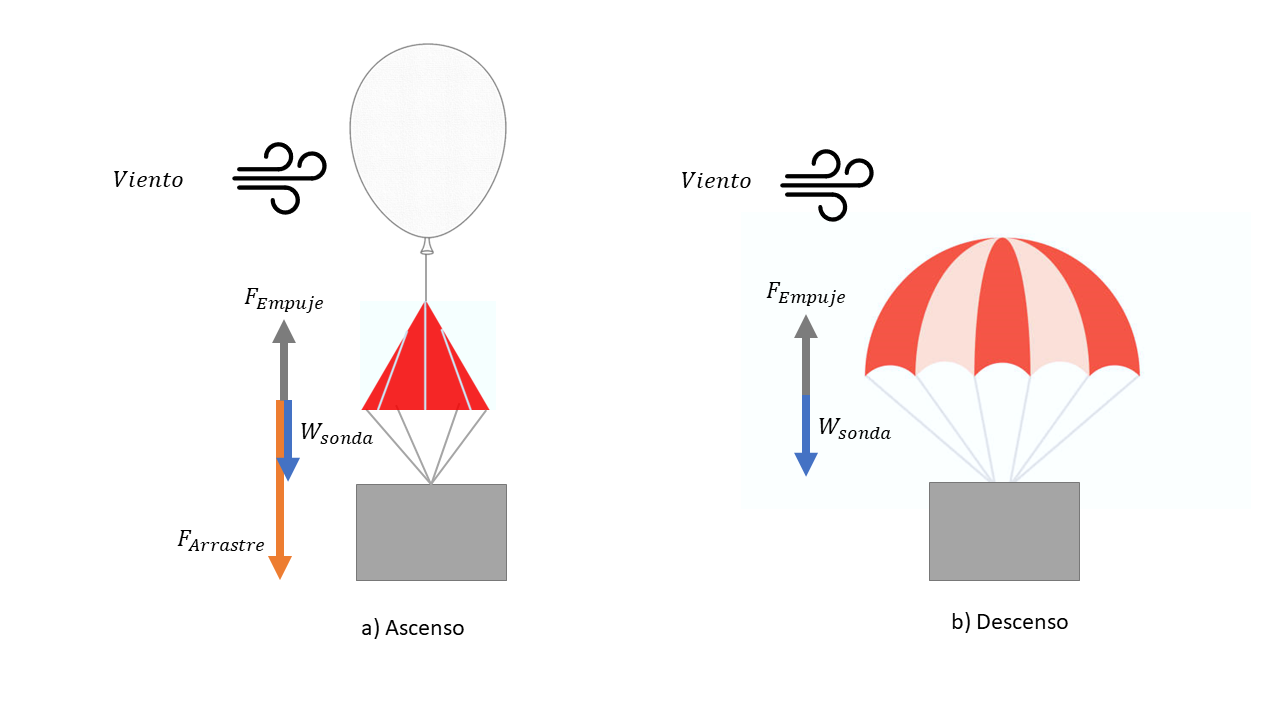
\includegraphics[width=0.75\linewidth]{document/figures/02_DCL_movimiento.png}
    \caption{Diagrama de cuerpo libre del sistema}
    \label{fig:dlc}
\end{figure}

\newpage

\subsection{Ecuación de movimiento vertical}

El movimiento vertical estará compuesto, por una parte, ascendente y una descendente, el cual en el primer instante representa cuando el globo está inflado y aún no ha explotado, el segundo  representa  donde todo el sistema comienza a caer en caída libre atado de un paracaídas. En figura \ref{fig:dlc} se muestra de forma representativa las fuerzas que actúan sobre el globo sonda.

\subsubsection{Ascenso}

Partiendo de un diagrama de cuerpo libre de figura \ref{fig:dlc} con un marco de referencia de un plano cartesiano tradicional,  en el cual se tiene las fuerzas que actúan sobre el globo sonda, se tendría que: existiría una peso $W_{Sonda}$ el cual actuaría negativo, una fuerza de empuje $F_{Empuje}$ encargada de que el globo ascienda y una fuerza resistiva de arrastre $F_{Arrastre}$ , generalizando  se tiene la siguiente ecuación:

\begin{equation}
    \label{eq:newton_ascenso}
  m \frac{\mathrm{d^2} z }{\mathrm{d} t^2}  =  F_{Empuje} - W_{Sonda} - F_{Arrastre}
\end{equation}

De este modo, contextualizando en ecuación \ref{eq:newton_ascenso}  con los modelos anteriores desarrollados y bibliografía consultada \cite{lsoda, ascenso_formula, ascenso_formula_2, constante_CD_y_formula_ascenso, simulador_chino}, se tiene:
\begin{equation}
    \label{eq:ascenso}
     ( m_{b} + m_{gas} + m_{pl} ) \; \frac{\mathrm{d^2} z }{\mathrm{d} t^2}  =  \rho_{atm} (z) \; V_{b} \; g (z) -( m_{b} + m_{pl} ) \; g(z) - \frac{1}{2} C_{D} \; \rho_{atm} \; S_{b} \; \left ( \frac{\mathrm{d} z }{\mathrm{d} t} \right )^{2}
\end{equation}
\textbf{Donde:}
\begin{itemize}
    \item $m_{b}$ es la masa del globo.
    \item $m_{gas}$ la masa del helio en el interior del globo.
    \item $m_{pl}$ es la masa de la carga útil o payload.
    \item $\rho_{atm}$ densidad atmosférica dada por la ISA, ver subsección \ref{ssct:simulacion:ISA_variables}.
    \item  $V_{b}$ volume del globo.
    \item $g$ es gravedad en función de la altitud, ver ecuación \ref{eq:gravedad}.
    \item $C_{D}$ y $S_{b}$  son el coeficiente de arrastre de una esfera y área transversal del globo.
\end{itemize}

En ecuación \ref{eq:ascenso} se comienza describiendo del lado izquierdo de la ecuación las diferentes masas que actúan en el sistema (masa del globo, masa del gas de elevación y masa del payload o carga útil respectivamente), luego de ello se tiene la presión, el volumen que se sustituye por ecuaciones de tabla \ref{tab:formulas_ISA} y ecuación  \ref{eq:volumen}, el  área que se sustituye por ecuación \ref{eq:area_transversal}. Además, se tiene la gravedad, coeficiente de arrastre y velocidad.

Como se hipotetiza que el globo sonda tiene una geometría esférica, el coeficiente de arrastre conocido que oscila entre $10^{4} $  y $10^{5}$ números de Reynolds \cite{constante_CD_y_formula_ascenso, Constatntes_CD_HAB}, por consiguiente en este trabajo se utiliza $C_{D} = 0.47$. 
 

\subsubsection{Descenso}

Una vez el globo llegó a su altura objetivo, este sufrirá una explosión la cual será afectada por la atracción gravitacional de la tierra, lo que hará que descienda en caída libre \cite{modelo_free_falling, redbull_free_falling}, este fenómeno se modela de la siguiente forma:
\begin{equation}
    \label{eq:newton_descenso}
  m \frac{\mathrm{d^2} z }{\mathrm{d} t^2}  =  F_{Arrastre} -W_{Sonda}
\end{equation}
Aplicando los modelos anteriores en ecuación \ref{eq:newton_descenso}, e ingresando los datos de entrada del paracaídas, tenemos que:

\begin{equation}
    \label{eq:descenso}
     ( m_{b} + m_{pl} ) \; \frac{\mathrm{d^2} z }{\mathrm{d} t^2}  =   \frac{1}{2} C_{D} \; \rho_{atm} \; S_{p} \; \left ( \frac{\mathrm{d} z }{\mathrm{d} t} \right )^{2} -( m_{b} + m_{pl} ) \; g(z) 
\end{equation}
\textbf{Donde:}
\begin{itemize}
    \item $m_{b}$ es la masa del globo.
    \item $m_{pl}$ es la masa de la carga útil o payload.
    \item $\rho_{atm}$ densidad atmosférica dada por la ISA, ver subsección \ref{ssct:simulacion:ISA_variables}. 
    \item $C_{D}$ y $S_{p}$  son el coeficiente de arrastre  y área transversal del paracaídas.
    \item     $g$ es gravedad en función de la altitud, ver ecuación \ref{eq:gravedad}.
\end{itemize}

En ecauación \ref{eq:descenso},  la fuerza de arrastre experimentada en el descenso es debido a la acción del paracaídas, y es positiva debido a que marco de referencia optado. La constante de arrastre $C_{D}$ oscila entre 0.5  y  0.8 según \cite{Constatntes_CD_HAB}, en este trabajo se utiliza $C_{D} = 0.8$, además que este dato no es proporcionado por el fabricante del paracaídas. 

\subsection{Ecuación de movimiento horizontal}

El movimiento horizontal es afectado por el viento  en el ascenso y descenso según la altura que se encuentre, ver figura \ref{fig:dlc}, para ello se toma los datos brindados por la National Oceanic and Atmospheric Administration (NOAA). Los datos proporcionados por la NOAA son discretos y están referenciados a alturas fijas, es por ello que es necesario una interpolación para obtener una función que nos permita conocer las condiciones del viento a diferentes alturas. Se trabaja con las siguientes ecuaciones basándose en \cite{lsoda}

\begin{equation}
    \label{eq:viento_x}
    \frac{\mathrm{d} x }{\mathrm{d} t} = - w(z) \cdot  \cos(\phi(z)) = u
\end{equation}

\begin{equation}
    \label{eq:viento_y}
    \frac{\mathrm{d} y }{\mathrm{d} t} = - w(z) \cdot \sin(\phi(z)) = v
\end{equation}

En este apartado, se utilizó el módulo getgfs  de Python \footnote{Más información de getgfs: \url{https://getgfs.readthedocs.io/en/latest/}}, que toma datos del modelo numérico de predicción Global Forecast System (GFS) desarrollado por la NOAA para obtener datos meteorológicos. Este módulo devuelve la interpolación de las componentes  U y V del viento. Al utilizar este módulo,  se elimina el desarrollo de las matemáticas trigonométricas en ecuaciones \ref{eq:viento_x} y \ref{eq:viento_y}, lo que permite realizar la integración de las ecuaciones diferenciales directamente.

Es relevante señalar que las componentes del viento $u$ y $v$ es el formato común en el cual se entregan  los datos del viento en meteorología\cite{lsoda}, a partir de ello se puede calcular la magnitud y dirección del viento. 
 
\section{Funcionamiento y resultados}

Se utilizó Jupyter Notebooks con Python para desarrollar el simulador de trayectoria ascendente y descendente, en el cual se ingresaron todos los datos iniciales y de entrada, luego se desarrolló cada modelo de forma individual para finalizar resolviendo las ecuaciones diferenciales \ref{eq:ascenso}, \ref{eq:descenso}, \ref{eq:viento_x}  y \ref{eq:viento_y}, utilizando la función de Scipy  solve\_ivp(). Dentro de esta función se utilizó el método de integración  "LSODA"  debido a los buenos resultados que se obtiene tal como lo indica \cite{lsoda}; las ecuaciones diferenciales son de segundo orden, fue necesario aplicar una reducción de orden para obtener las soluciones debido a que Python no posee una forma directa para resolverlas.  Además,  en las ecuaciones \ref{eq:viento_x} y \ref{eq:viento_y} se utiliza el módulo de Python pyproj para homogeneizar las unidades  de la superficie de la tierra sobre un plano, transformando la latitud y la longitud de su representación decimal mostrada en tabla \ref{tab:datos_start_input} a unidades de metros.

Una vez realizada la resolución matemática, se obtuvo datos de posición y tiempo del sistema, se sustituyeron en los modelos y ecuaciones pertinentes, recalculándolos debido a que la función solve\_ivp() no devuelve estos valores, y así se obtuvo los datos correspondientes en cada instante y posición como son la presión, temperatura, diámetro del globo, etc.  

\newpage
Por lo anterior,  el simulador representa el comportamiento de la trayectoria descendente y ascendente. Véase las siguientes tablas \ref{tab:ascenso_frag_datos_generados} y \ref{tab:descenso_frag_datos_generados} que contiene una muestra de los datos generados del simulador, estas tablas fueron creadas a partir de almacenar los datos en archivos .csv\footnote{Los archivos .csv se pueden consultar visitando los anexos \ref{chp:anexo:source_thesis}}, que son la base de donde se hace los análisis en el siguiente capítulo.

\vspace{1 cm}

\textbf{Nota:} el código fuente desarrollado para la simulación de trayectoria  se detalla en el anexo \ref{chp:anexo:source_thesis}. Además, es accesible lo realizado en capítulo \ref{chp:03_eda} y toda la documentación perteneciente a este trabajo \footnote{Consulte rápidamente el código fuente, en la siguiente URL: \url{https://github.com/osminlab/Proyec_Gda_Simula_PCB_Nav}}.

% ------------------------------------------------------------------
% Framento de simulación en tablas, con contenido rotado
% ------------------------------------------------------------------

\begin{landscape}
    % TABLA ASCENSO
    \begin{table}
\small
\centering
\caption{Ascenso, fragmento de los datos generados en simulación.}
\label{tab:ascenso_frag_datos_generados}
\begin{tabular}{cccccccccccc}
\toprule
\textbf{t [s]} & \textbf{Lat. ($\phi$)} & \textbf{Long. ($\lambda$)} & \textbf{Alt. (z) [km]} & \textbf{$dz/dt$ [m/s]} & \textbf{u [m/s]} & \textbf{v [m/s]} & \textbf{T [°C]} & \textbf{P [hPa]} & \textbf{$\rho$ [kg/m³]} & \textbf{g [m/s²]} & \textbf{d [m]} \\
\midrule
             0 &                13.8088 &                    -89.329 &                    0.5 &                    0.0 &              0.0 &              0.4 &            11.7 &            954.2 &                     1.2 &               9.8 &            1.9 \\
             1 &                13.8088 &                    -89.329 &                   0.51 &                    1.9 &              0.0 &              0.4 &            11.7 &            954.0 &                     1.2 &               9.8 &            1.9 \\
             2 &                13.8088 &                    -89.329 &                   0.51 &                    2.8 &              0.0 &              0.4 &            11.7 &            953.8 &                     1.2 &               9.8 &            1.9 \\
             3 &                13.8088 &                    -89.329 &                   0.51 &                    3.2 &              0.0 &              0.4 &            11.7 &            953.4 &                     1.2 &               9.8 &            1.9 \\
             4 &                13.8088 &                    -89.329 &                   0.51 &                    3.3 &              0.0 &              0.4 &            11.7 &            953.0 &                     1.2 &               9.8 &            1.9 \\
             5 &                13.8088 &                    -89.329 &                   0.52 &                    3.3 &              0.0 &              0.4 &            11.6 &            952.7 &                     1.2 &               9.8 &            1.9 \\
             . &                      . &                          . &                      . &                      . &                . &                . &               . &                . &                       . &                 . &              . \\
             . &                      . &                          . &                      . &                      . &                . &                . &               . &                . &                       . &                 . &              . \\
             . &                      . &                          . &                      . &                      . &                . &                . &               . &                . &                       . &                 . &              . \\
          3333 &                13.8752 &                   -89.3277 &                  12.72 &                    4.2 &             -4.6 &              3.3 &           -56.5 &            173.3 &                     0.3 &               9.8 &            3.0 \\
          3334 &                13.8752 &                   -89.3277 &                  12.72 &                    4.2 &             -4.6 &              3.3 &           -56.5 &            173.2 &                     0.3 &               9.8 &            3.0 \\
          3335 &                13.8752 &                   -89.3277 &                  12.73 &                    4.2 &             -4.6 &              3.3 &           -56.5 &            173.1 &                     0.3 &               9.8 &            3.0 \\
          3336 &                13.8752 &                   -89.3277 &                  12.73 &                    4.2 &             -4.6 &              3.3 &           -56.5 &            173.0 &                     0.3 &               9.8 &            3.0 \\
          3337 &                13.8751 &                   -89.3277 &                  12.73 &                    4.2 &             -4.6 &              3.3 &           -56.5 &            172.9 &                     0.3 &               9.8 &            3.0 \\
          3338 &                13.8751 &                   -89.3277 &                  12.74 &                    4.2 &             -4.6 &              3.3 &           -56.5 &            172.8 &                     0.3 &               9.8 &            3.0 \\
             . &                      . &                          . &                      . &                      . &                . &                . &               . &                . &                       . &                 . &              . \\
             . &                      . &                          . &                      . &                      . &                . &                . &               . &                . &                       . &                 . &              . \\
             . &                      . &                          . &                      . &                      . &                . &                . &               . &                . &                       . &                 . &              . \\
          6660 &                  13.87 &                   -89.3244 &                  29.96 &                    6.5 &            -29.2 &              3.6 &           -46.6 &             12.1 &                     0.0 &               9.7 &            7.5 \\
          6661 &                  13.87 &                   -89.3244 &                  29.97 &                    6.5 &            -29.2 &              3.6 &           -46.6 &             12.1 &                     0.0 &               9.7 &            7.5 \\
          6662 &                13.8699 &                   -89.3244 &                  29.97 &                    6.5 &            -29.2 &              3.6 &           -46.6 &             12.0 &                     0.0 &               9.7 &            7.5 \\
          6663 &                13.8699 &                   -89.3244 &                  29.98 &                    6.5 &            -29.2 &              3.7 &           -46.6 &             12.0 &                     0.0 &               9.7 &            7.5 \\
          6664 &                13.8699 &                   -89.3244 &                  29.99 &                    6.5 &            -29.2 &              3.7 &           -46.6 &             12.0 &                     0.0 &               9.7 &            7.5 \\
          6665 &                13.8699 &                   -89.3244 &                  29.99 &                    6.5 &            -29.2 &              3.7 &           -46.6 &             12.0 &                     0.0 &               9.7 &            7.5 \\
\bottomrule
\end{tabular}
\end{table}

\end{landscape}

\begin{landscape}
    % TABLA DESCENSO
    \begin{table}
\footnotesize
\centering
\caption{Descenso, fragmento de los datos generados en simulación.}
\label{tab:descenso_frag_datos_generados}
\begin{tabular}{cccccccccccc}
\toprule
\textbf{t [s]} & \textbf{Lat. ($\phi$)} & \textbf{Long. ($\lambda$)} & \textbf{Alt. (z) [km]} & \textbf{$dz/dt$ [m/s]} & \textbf{u [m/s]} & \textbf{v [m/s]} & \textbf{T [°C]} & \textbf{P [hPa]} & \textbf{$\rho$ [kg/m³]} & \textbf{g [m/s²]} & \textbf{d [m]} \\
\midrule
          6665 &                13.8699 &                   -89.3244 &                  29.99 &                    6.5 &            -29.2 &              3.7 &           -46.6 &             12.0 &                     0.0 &               9.7 &            0.0 \\
          6666 &                13.8698 &                   -89.3244 &                   30.0 &                   -3.1 &            -29.2 &              3.7 &           -46.6 &             12.0 &                     0.0 &               9.7 &            0.0 \\
          6667 &                13.8698 &                   -89.3244 &                  29.99 &                  -12.5 &            -29.2 &              3.7 &           -46.6 &             12.0 &                     0.0 &               9.7 &            0.0 \\
          6668 &                13.8698 &                   -89.3244 &                  29.97 &                  -21.0 &            -29.2 &              3.6 &           -46.6 &             12.1 &                     0.0 &               9.7 &            0.0 \\
          6669 &                13.8697 &                   -89.3244 &                  29.95 &                  -28.1 &            -29.2 &              3.6 &           -46.6 &             12.1 &                     0.0 &               9.7 &            0.0 \\
          6670 &                13.8697 &                   -89.3244 &                  29.92 &                  -33.6 &            -29.2 &              3.5 &           -46.6 &             12.2 &                     0.0 &               9.7 &            0.0 \\
             . &                      . &                          . &                      . &                      . &                . &                . &               . &                . &                       . &                 . &              . \\
             . &                      . &                          . &                      . &                      . &                . &                . &               . &                . &                       . &                 . &              . \\
             . &                      . &                          . &                      . &                      . &                . &                . &               . &                . &                       . &                 . &              . \\
          7843 &                13.8769 &                   -89.3236 &                   8.49 &                   -9.2 &             -7.6 &            -11.3 &           -40.2 &            332.3 &                     0.5 &               9.8 &            0.0 \\
          7844 &                 13.877 &                   -89.3236 &                   8.48 &                   -9.2 &             -7.6 &            -11.3 &           -40.1 &            332.8 &                     0.5 &               9.8 &            0.0 \\
          7845 &                13.8771 &                   -89.3236 &                   8.47 &                   -9.2 &             -7.6 &            -11.2 &           -40.1 &            333.2 &                     0.5 &               9.8 &            0.0 \\
          7846 &                13.8772 &                   -89.3236 &                   8.47 &                   -9.2 &             -7.6 &            -11.1 &           -40.0 &            333.7 &                     0.5 &               9.8 &            0.0 \\
          7847 &                13.8773 &                   -89.3236 &                   8.46 &                   -9.2 &             -7.6 &            -11.1 &           -40.0 &            334.1 &                     0.5 &               9.8 &            0.0 \\
          7848 &                13.8774 &                   -89.3236 &                   8.45 &                   -9.2 &             -7.6 &            -11.0 &           -39.9 &            334.6 &                     0.5 &               9.8 &            0.0 \\
             . &                      . &                          . &                      . &                      . &                . &                . &               . &                . &                       . &                 . &              . \\
             . &                      . &                          . &                      . &                      . &                . &                . &               . &                . &                       . &                 . &              . \\
             . &                      . &                          . &                      . &                      . &                . &                . &               . &                . &                       . &                 . &              . \\
          9014 &                13.8929 &                   -89.3232 &                   0.03 &                   -5.9 &              0.0 &              0.4 &            14.8 &           1009.4 &                     1.2 &               9.8 &            0.0 \\
          9015 &                13.8929 &                   -89.3232 &                   0.03 &                   -5.9 &              0.0 &              0.4 &            14.8 &           1010.1 &                     1.2 &               9.8 &            0.0 \\
          9016 &                13.8929 &                   -89.3232 &                   0.02 &                   -5.9 &              0.0 &              0.4 &            14.9 &           1010.8 &                     1.2 &               9.8 &            0.0 \\
          9017 &                13.8929 &                   -89.3232 &                   0.01 &                   -5.9 &              0.0 &              0.4 &            14.9 &           1011.5 &                     1.2 &               9.8 &            0.0 \\
          9018 &                13.8929 &                   -89.3232 &                   0.01 &                   -5.9 &              0.0 &              0.4 &            14.9 &           1012.3 &                     1.2 &               9.8 &            0.0 \\
          9019 &                13.8929 &                   -89.3232 &                    0.0 &                   -5.9 &              0.0 &              0.4 &            15.0 &           1013.0 &                     1.2 &               9.8 &            0.0 \\
\bottomrule
\end{tabular}
\end{table}
 
\end{landscape}


\chapter{Análisis Exploratorio de Datos} \label{chp:03_eda}

\vspace{0.2cm}

 El principal propósito de este capítulo es analizar a través de técnicas estadísticas y visualización de datos,  se busca  relacionar los diferentes parámetros, observar tendencias, explorar anomalías, patrones, identificar correlaciones y obtener información significativa que permite comprender mejor los fenómenos y sus influencias asociados con el vuelo de globos sonda. El exploratorio se desarrolla a partir de la simulación de trayectoria generada, entre los datos generados se encuentra la temperatura,  presión, velocidad, tiempo, viento y la posición geográfica del globo en términos de latitud y longitud.  Estos datos ofrecen una visión detallada y completa de las condiciones  o situaciones a las que el globo sonda se expone a lo largo de su trayectoria, según las hipótesis del modelo en sección \ref{sct:simulacion:hipotesis}.

\vspace{0.4cm}

A lo largo de este capítulo \ref{chp:03_eda}  se realizaron transformaciones o cálculos adicionales para crear nuevas características derivadas  de los datos existentes o conversiones de unidades para facilitar la compresión y análisis. Además, los datos fueron desarrollados de tal forma no existieran datos nulos, existiendo la misma cantidad de ítems en cada fila y columna, por lo tanto, no es necesario detectar ni manejar valores nulos o atípicos.

\newpage

\section{Exploratorio estadística descriptiva}

Las variables continuas que a continuación se describen son las generadas por el modelo de simulación de trayectoria:

\vspace{0.4 cm}

\begin{enumerate}
    \item \textbf{Tiempo:} unidad de sucesos donde la trayectoria de ascenso y descenso se describe. 
    \item \textbf{Latitud} ($\phi$): coordenada geográfica sobre la posición norte-sur donde se ubica la sonda en la superficie de la tierra. 
    \item 	 \textbf{Longitud} ($\lambda$): coordenada geográfica sobre la posición este-oeste donde se ubica la sonda en la superficie de la tierra. 
    \item 	\textbf{Altitud (z):} elevación vertical sobre la superficie de la tierra donde se ubica la sonda.
    \item 	\textbf{Velocidad vertical ($dz/dt$):} cambio de posición sobre la elevación vertical de la sonda por unidad de tiempo.
    \item   \textbf{Velocidad del viento U:} componente de viento paralela a la latitud. Es positiva de oeste a este. 
    \item 	\textbf{Velocidad del viento V:}  componente de viento paralela a la longitud. Es positiva de sur a norte.
    \item 	\textbf{Temperatura:} temperatura atmosférica basada en la ISA a lo largo de su posición espacial y temporal en la trayectoria.
    \item   \textbf{Presión:} presión atmosférica basada en la ISA a lo largo de su posición espacial y temporal en la trayectoria.
    \item	\textbf{Densidad:} densidad atmosférica a lo largo de su posición espacial y temporal en la trayectoria.
    \item 	\textbf{Gravedad:} intensidad del campo gravitatorio en función de la altitud en la trayectoria.
    \item  \textbf{Diámetro del Globo:} longitud transversal del globo. De valor cero en el descenso debido a su exposición.
\end{enumerate}

\vspace{0.6 cm}

Se calcularon las estadísticas descriptivas de las doce variables anteriormente detalladas, los  resultados se pueden ver  en tabla \ref{tab:desciptivo_ascenso} y \ref{tab:desciptivo_descenso}; en las tablas se muestra la distribución de estas variables y proporciona información sobre tendencia central, dispersión y rango, estas variables que se incluye son:  media, desviación típica o estándar,  valor mínimo (mín), primer cuartil (25\% ), mediana (50\%), tercer cuartil (75\%) y valor máximo (máx).

% ------------------------------------------------------------------
%   TABLAS ESTADÍSTICAS DESCRIPTIVAS
% ------------------------------------------------------------------
\begin{landscape}

    %   ASCENSO
    \begin{table}
\small
\centering
\caption{Estadística descriptiva ascenso.}
\label{tab:desciptivo_ascenso}
\begin{tabular}{cccccccccccc}
\toprule
{} &  \textbf{Media} &  \textbf{Desviación típica} &  \textbf{Min} &  \textbf{25\%} &  \textbf{50\%} &  \textbf{75\%} &  \textbf{Máx} \\
\midrule
\textbf{\textbf{Tiempo [min]}        } &        55.54167 &                    32.07421 &       0.00000 &       27.77083 &       55.54167 &       83.31250 &     111.08333 \\
\textbf{\textbf{Latitud ($\phi$)}    } &        13.85097 &                     0.02472 &      13.80770 &       13.82157 &       13.85663 &       13.87343 &      13.88286 \\
\textbf{\textbf{Longitud ($\lambda$)}} &       -89.32764 &                     0.00109 &     -89.32899 &      -89.32861 &      -89.32774 &      -89.32714 &     -89.32439 \\
\textbf{\textbf{Altitud (z) [km]}    } &        13.53558 &                     8.36012 &       0.50400 &        6.25319 &       12.71488 &       20.38154 &      29.99412 \\
\textbf{\textbf{Vel. Vertical [m/s]} } &         4.41683 &                     0.91557 &       0.00000 &        3.63057 &        4.16845 &        5.08576 &       6.53168 \\
\textbf{\textbf{Viento U [m/s]}      } &        -6.43619 &                     7.06341 &     -29.22083 &       -7.02784 &       -3.73740 &       -2.72217 &       0.12773 \\
\textbf{\textbf{Viento V [m/s]}      } &        -0.90501 &                     3.27907 &     -12.06565 &       -2.77407 &        0.03555 &        0.96788 &       4.51644 \\
\textbf{\textbf{Temperatura [°C]}    } &       -39.86431 &                    21.04598 &     -56.62071 &      -56.50000 &      -50.59204 &      -25.64574 &      11.72400 \\
\textbf{\textbf{Presión [hPa]}       } &       278.83265 &                   268.33053 &      12.01172 &       52.08537 &      173.39945 &      456.37325 &     954.15967 \\
\textbf{\textbf{Densidad [kg/m³]}    } &         0.38779 &                     0.33925 &       0.01847 &        0.08363 &        0.27883 &        0.64238 &       1.16688 \\
\textbf{\textbf{Gravedad [m/s²]}     } &         9.76516 &                     0.02556 &       9.71496 &        9.74420 &        9.76762 &        9.78743 &       9.80510 \\
\textbf{\textbf{Diámetro Globo [m]}  } &         3.57101 &                     1.52970 &       1.88882 &        2.30463 &        3.04381 &        4.54716 &       7.52292 \\
\bottomrule
\end{tabular}
\end{table}

    %  DESCENSO
    \begin{table}
\small
\centering
\caption{Estadística descriptiva descenso.}
\label{tab:desciptivo_descenso}
\begin{tabular}{cccccccccccc}
\toprule
{} &  \textbf{Media} &  \textbf{Desviación típica} &  \textbf{Min} &  \textbf{25\%} &  \textbf{50\%} &  \textbf{75\%} &  \textbf{Máx} \\
\midrule
\textbf{\textbf{Tiempo [min]}        } &       130.70000 &                    11.33290 &     111.08333 &      120.89167 &      130.70000 &      140.50833 &     150.31667 \\
\textbf{\textbf{Latitud ($\phi$)}    } &        13.87943 &                     0.01062 &      13.86401 &       13.86943 &       13.87684 &       13.88892 &      13.89368 \\
\textbf{\textbf{Longitud ($\lambda$)}} &       -89.32359 &                     0.00030 &     -89.32439 &      -89.32384 &      -89.32358 &      -89.32328 &     -89.32323 \\
\textbf{\textbf{Altitud (z) [km]}    } &        10.18119 &                     7.68314 &       0.00246 &        3.78148 &        8.50208 &       15.22393 &      29.99583 \\
\textbf{\textbf{Vel. Vertical [m/s]} } &       -12.72221 &                     8.57864 &     -45.78658 &      -14.85339 &       -9.17031 &       -7.06163 &       6.53168 \\
\textbf{\textbf{Viento U [m/s]}      } &        -4.64714 &                     5.30650 &     -29.22116 &       -4.96890 &       -3.33289 &       -2.16755 &       0.12705 \\
\textbf{\textbf{Viento V [m/s]}      } &        -1.07031 &                     3.27182 &     -12.06136 &       -2.78589 &       -0.09935 &        0.85241 &       4.51088 \\
\textbf{\textbf{Temperatura [°C]}    } &       -32.04419 &                    24.41396 &     -56.61399 &      -56.50000 &      -40.26352 &       -9.57964 &      14.98399 \\
\textbf{\textbf{Presión [hPa]}       } &       391.38992 &                   299.08436 &      12.00867 &      116.98481 &      331.87727 &      634.51183 &    1012.95419 \\
\textbf{\textbf{Densidad [kg/m³]}    } &         0.53004 &                     0.36444 &       0.01846 &        0.18812 &        0.49647 &        0.83869 &       1.22477 \\
\textbf{\textbf{Gravedad [m/s²]}     } &         9.77542 &                     0.02351 &       9.71496 &        9.75995 &        9.78053 &        9.79502 &       9.80664 \\
\textbf{\textbf{Diámetro Globo [m]}  } &         0.00000 &                     0.00000 &       0.00000 &        0.00000 &        0.00000 &        0.00000 &       0.00000 \\
\bottomrule
\end{tabular}
\end{table}
  
    
\end{landscape}

  
\subsection{Generalidades}

En tabla \ref{tab:desciptivo_ascenso} y  \ref{tab:desciptivo_descenso} se presentan información estadística que proporciona una descripción cuantitativa de la trayectoria ascendente y descendente respectivamente del globo sonda en términos de tiempo, coordenadas geográficas, altitud, velocidades en diferentes direcciones, condiciones atmosféricas y una característica física del globo.

El tiempo, la posición espacial y condiciones atmosféricas son los datos más importantes, es por ello que los datos extremos que proporcionen estas variables dan una idea general de como son las tendencias y la distribución; esta información muestra lo que puede generar inquietud en la misión del globo sonda. Dentro de las condiciones atmosféricas se comporta igual a lo largo del ascenso y descenso debido al comportamiento de la ISA que solo es función de la altitud, las diferencias en las tablas son debidas al tiempo en que está expuesta en las diferentes capas de atmósfera. 


\subsection{Aspectos relevantes ascenso}

De la tabla \ref{tab:desciptivo_ascenso} se puede deducir:
    
    \begin{itemize}
        \item \textbf{\textit{Tiempo:}} el valor máximo registrado es de 111 minutos, que corresponde al tiempo en que tardó el globo-sonda durante la fase de ascenso de la misión.
        \item \textbf{\textit{Posición (latitud, longitud y altitud):}  }las medias de la latitud y longitud muestran que el globo siempre estará en territorio salvadoreño en el ascenso, las variaciones de estas magnitudes son debidas a los vientos U y V. La altitud representa un desarrollo bastante constante, eso se corrobora con la velocidad vertical.
        \item \textbf{\textit{Velocidades (vertical, U y V):}}  la velocidad vertical posee una desviación de 0.92 m/s con una media de 4.42 m/s  que no presentan una alta variabilidad en función a los datos, desde el reposo hasta su velocidad máxima hasta la explosión del globo se observa un rango de los 4 a 6 m/s, es decir,  que es muy constante tal como indicaba el estudio \cite{ascentRate_weatherBallon} en velocidades verticales ascendentes. En cuanto a las velocidades horizontales U y V,  se percibe una alta variabilidad y aleatoriedad debido a su naturaleza estocástica. 
        \item \textbf{\textit{Atmosféricos (temperatura, presión y densidad) :}} la temperatura y la presión muestran estar en condiciones extremas, se puede ver en sus cuartiles y además posee una alta desviación estándar, para la temperatura la media es de temperatura es de -39.90 °C  con ± 21  °C  y la presión es de 278.8 hPa con  ± 268.3 hPa. Por otro lado, la densidad es función de la temperatura y presión, por lo que decae en todo el trayecto.
        \item  \textbf{\textit{Gravedad:}} el valor promedio o media fue de  9.765 m/s² durante el ascenso y la desviación estándar de 0.0255 m/s² muestra que los datos no presentan variación significativa, lo que siguiere que es casi constante la influencia de la gravedad sobre el sistema globo-sonda.
        \item  \textbf{\textit{Diámetro del globo:}} se evidencia la evolución gradual, el cual es un comportamiento esperado, según el cual se observa que el  diámetro inicial cambia lentamente hasta el tercer cuartil (75\%, con valor de 4.547 m), y luego sucede un crecimiento vertiginoso de casi duplicar su longitud hasta la explosión en 7.5 m debido a la diferencia de presión atmoferica.
    \end{itemize}

\subsection{Aspectos relevantes descenso} \label{ssct:eda:aspectos_descenso} 

De la tabla \ref{tab:desciptivo_descenso} se puede deducir:
    
    \begin{itemize}

        \item \textbf{\textit{Tiempo:}} los valores mínimo y máximo registrados son 111 minutos y 150.3 minutos, respectivamente, la diferencia da como resultado la duración del descenso que es de 39 minutos. Por último, se observa disminución  temporal respecto al ascenso debido a que la fuerza gravedad hace mayor acción  y hay poco dominio/presencia de fuerzas resistivas, ver ecuación \ref{eq:descenso}.
        \item \textbf{\textit{Posición (latitud, longitud y altitud):}}  la latitud y longitud en su desviación estándar muestran una menor variabilidad que en el ascenso, siendo 0.01062 y 0.00030 respectivamente. En cambio, la altitud representa un incremento en su desarrollo descendente con respeto al ascendente, corroborándose lo anterior en la velocidad vertical.
        \item \textbf{\textit{Velocidad (vertical, U y V):}}  la velocidad vertical sufre un cambio en su dirección, pasando de la velocidad máxima del ascenso (6.50 m/s) a tener una velocidad promedio de -12.70 m/s con una alta desviación típica de ± 8.60 m/s lo que sugiere una desaceleración. En contraste, las velocidades horizontales de U y V muestran un comportamiento bastante similar a los datos de la tabla del ascenso, solo cambian los datos de la media y la desviación estándar.  Todo lo anterior debido al cambio en la posición y tiempo.
        \item \textbf{\textit{Atmosféricos  (temperatura, presión y densidad):}}  lo explicado en la subsección \ref{ssct:eda:aspectos_descenso} son aplicables aquí, lo único que cambie es el tiempo de exposición de las variables atmosféricas, siendo este tiempo menor. 
        \item \textbf{\textit{Gravedad:}}  No indica mayor información que la expuesta en el análisis del ascenso, solamente cambia el tiempo en que toma en experimentar el cambio en el aumento de la gravedad.
        \item \textbf{\textit{Diámetro del globo:}}  En el descenso, el diámetro del globo se registra como 0.00 m debido a la explosión que lo elimina del sistema por completo.
    \end{itemize}
        
\newpage

\section{Visualización de datos}

En general, las visualizaciones  permite analizar diferentes aspectos del movimiento para identificar patrones, tendencias, cambios bruscos y posibles puntos de interés a lo largo de la trayectoria.


\subsection{Posición vs Tiempo}

Se inspecciona la relación entre la posición espacial del globo sonda y el tiempo transcurrido durante su vuelo. Esta representación nos proporciona una visión dinámica de la trayectoria seguida por el globo a medida que asciende y desciende a través de la atmósfera en  su posición geográfica y de altitud.

En la figura \ref{fig:3d_trayectoria} se hace la representación 3D de la posición espacial y se muestra el tiempo que la sonda tarda a lo largo de su trayectoria.  Se logra ver un comportamiento suave y curvo en su ascenso, así mismo, al momento de descender se observa comportamiento en caída libre que es influenciado por corrientes de viento desplazándolo. Las corrientes de viento son las encargadas de generar el comportamiento horizontal del movimiento, en cambio, el movimiento vertical es debido a la fuerza de empuje ocasionada por el gas de elevación  y también a la atracción gravitacional.

\begin{figure}[!h]
    \centering
    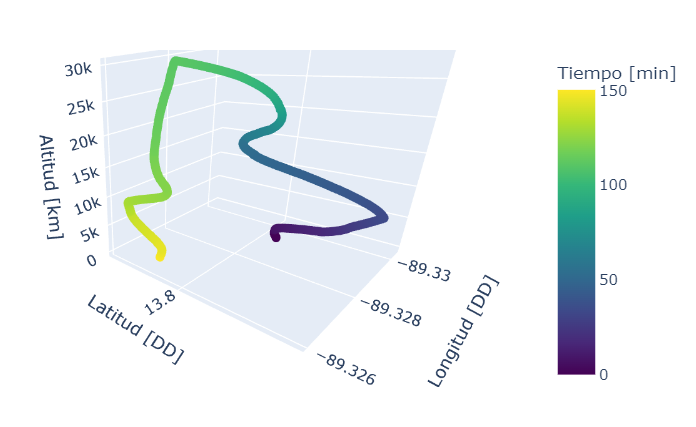
\includegraphics[width=0.75\linewidth]{document/figures/03_simu_grafico_3D_trayectoria.png}
    \caption{Vista 3D de la simulación de trayectoria}
    \label{fig:3d_trayectoria}
\end{figure}

\newpage

\begin{figure}[ht]
    \centering
    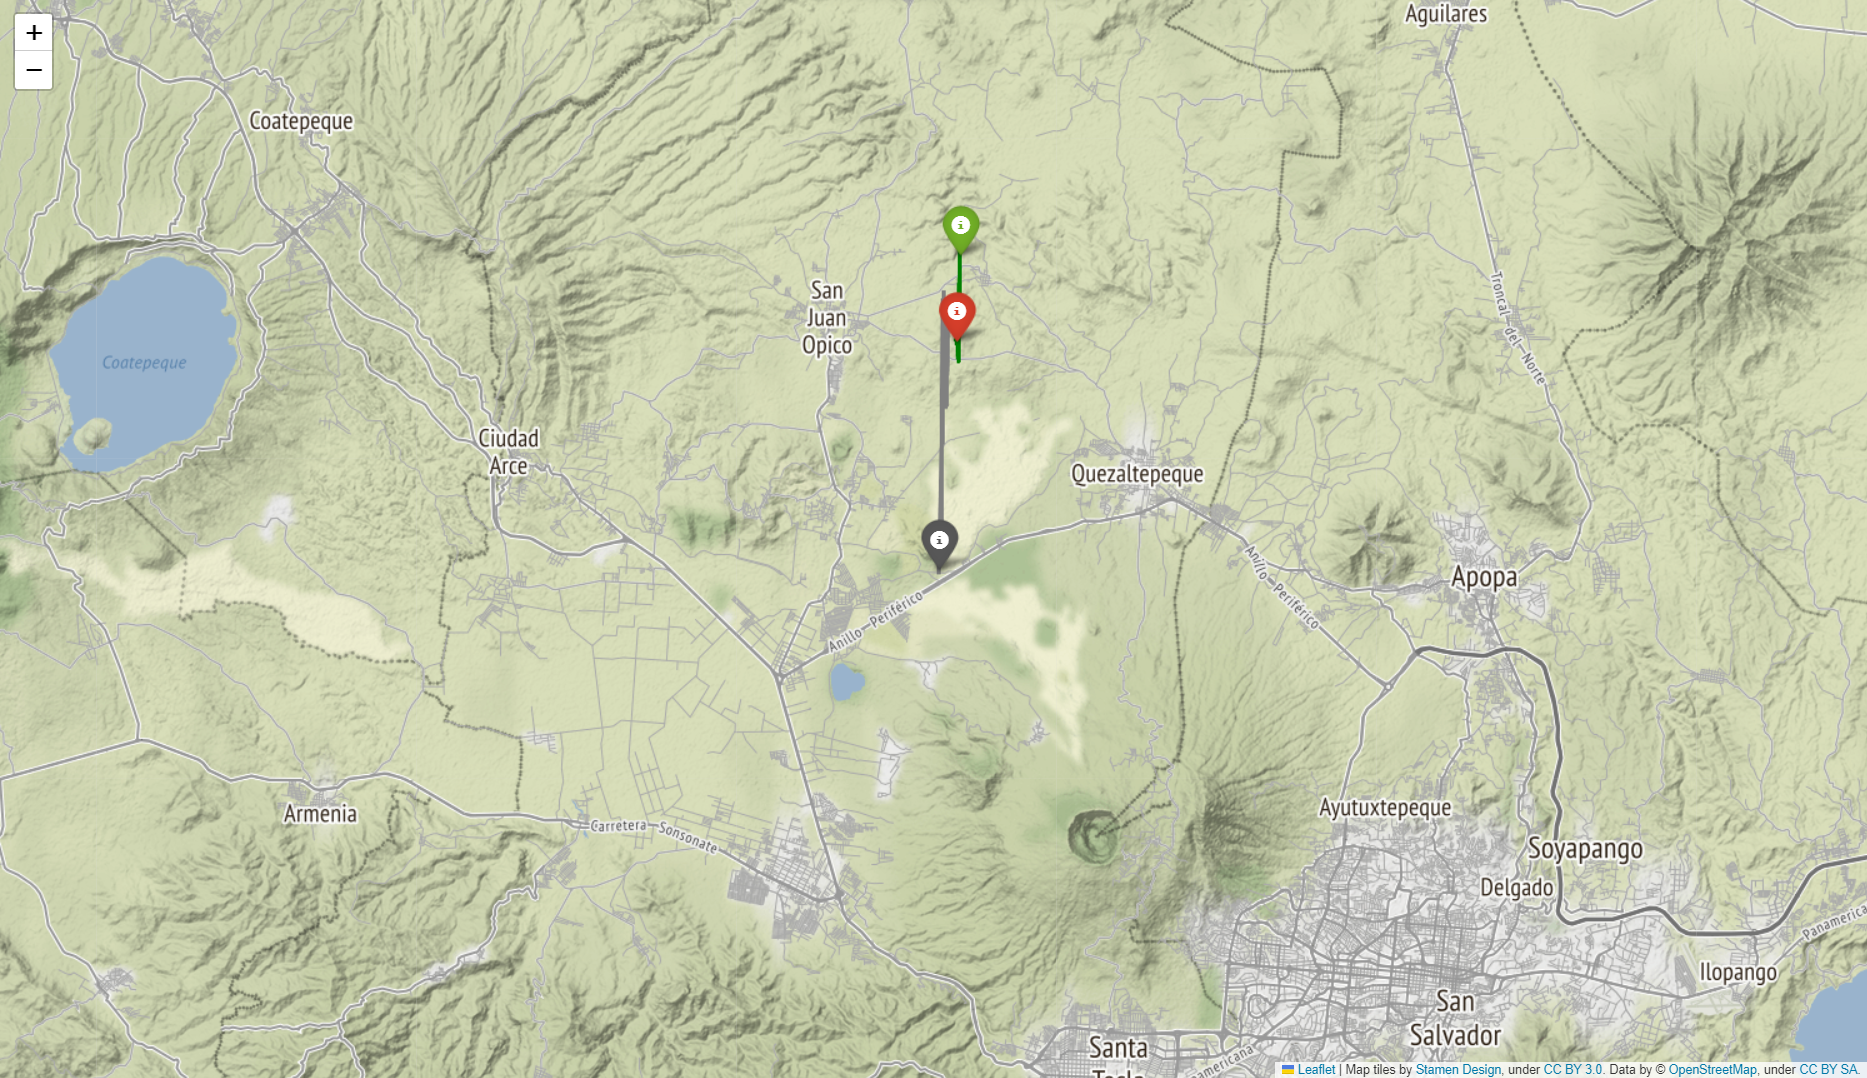
\includegraphics[width=0.9\linewidth]{document/figures/03_mapa.png}
    \caption{Vista desde un mapa geográfico de la simulación.}
    \label{fig:mapa}
\end{figure}

En figura \ref{fig:mapa} está presente la trayectoria de la sonda sobre plano horizontal que recorre distancia lineal aproximada de 9.2 km desde el punto de lanzamiento al de aterrizaje, mostrada concretamente un mapa geográfico\footnote{Se usó mapas de OpenStreet, con el módulo de Pyhton "Folium"} proporciona una visualización clara de los puntos clave de su viaje: el lugar de lanzamiento, la explosión  y el punto de aterrizaje.

\textbf{El primer punto de interés,  marcador gris}, representa el lugar de lanzamiento del globo sonda. Esta ubicación inicial es seleccionada arbitrariamente por poseer un horizonte despejado. Vale comentar, que siempre para realizar esta operación es crucial considerar las condiciones meteorológicas en el momento del lanzamiento, siendo en este trabajo obviado.

\textbf{El siguiente punto, marcador rojo}, corresponde al lugar donde tiene acción  la explosión del globo sonda y el inicio de la caída libre. Esta explosión ocurre generalmente cuando el globo ha alcanzado una altitud objetiva de la misión o cuando las características del globo son superadas por las variables atmosféricas existentes a las que fue diseñado. 

\textbf{Finalmente, el punto verde,}  índica el lugar de aterrizaje del globo sonda, este es el punto más crucial y es necesario una precisión aceptable de simulación para determinar una recuperación exitosa del globo sonda y los instrumento que transporte.

\newpage

\begin{figure}[ht]
    \centering
    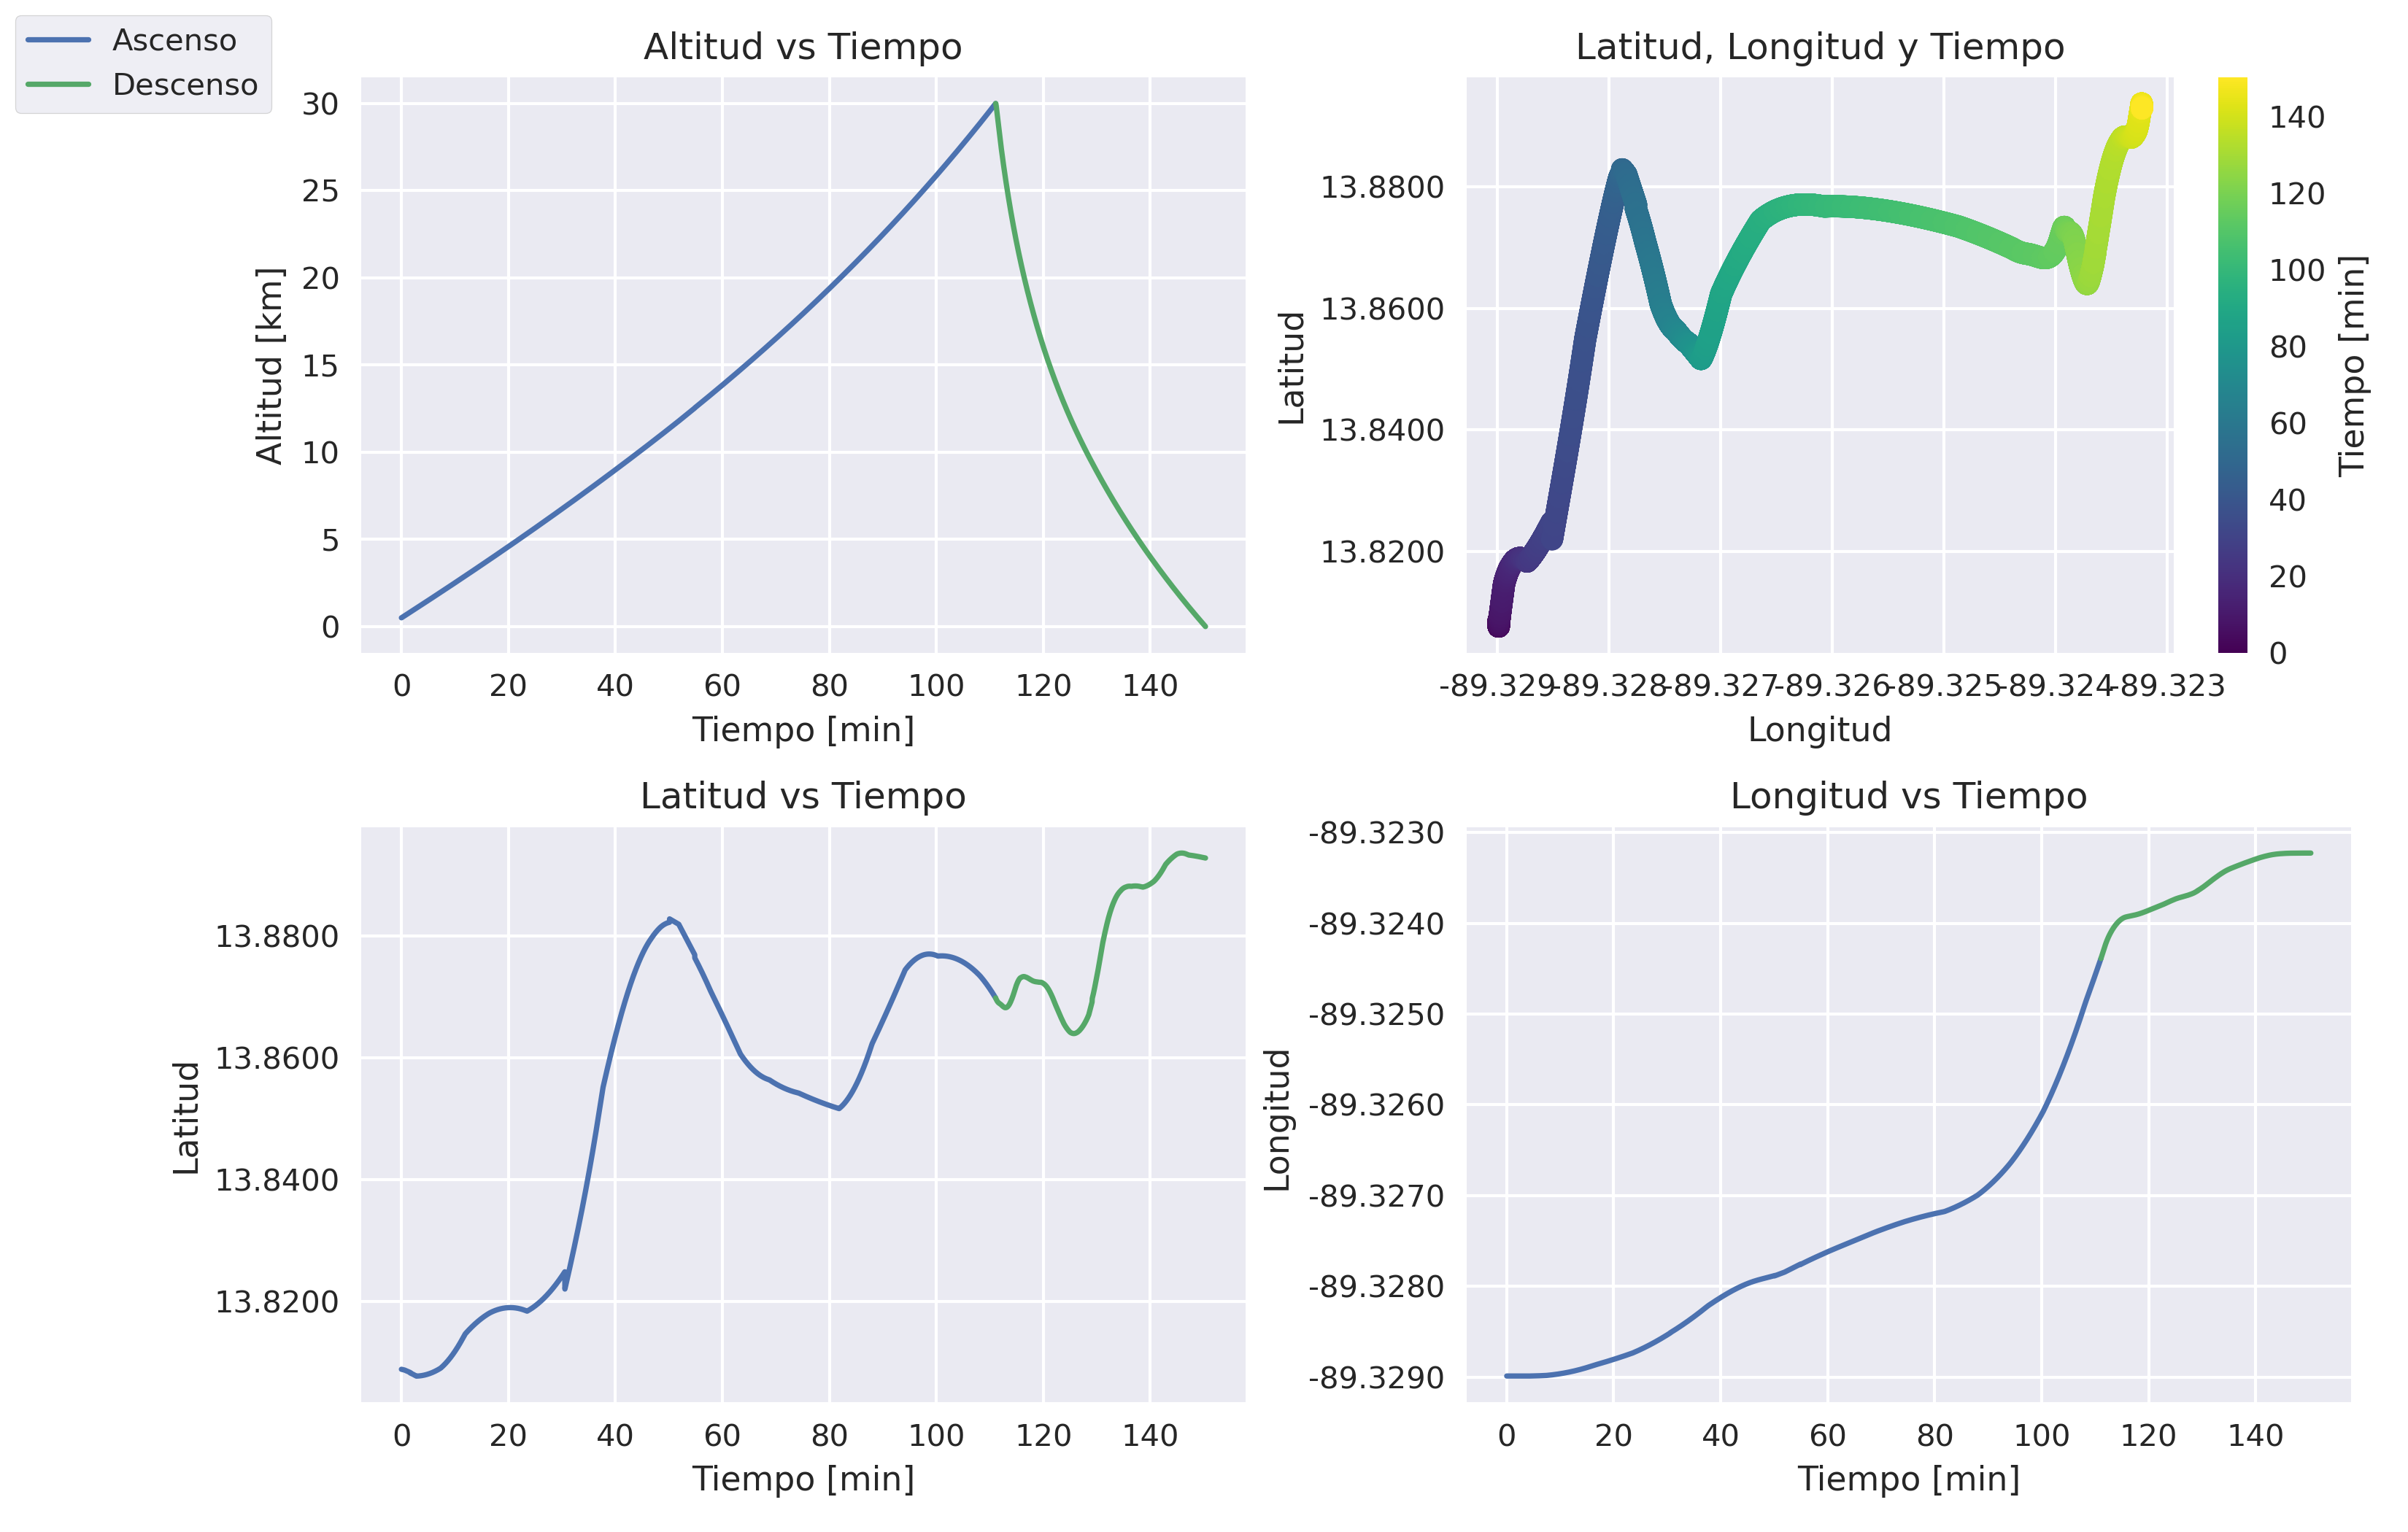
\includegraphics[width=0.93\linewidth]{document/figures/03_plano_posicion_vs_tiempo.png}
    \caption{Vista desde un plano de la posición y tiempo}
    \label{fig:posicion_vs_tiempo}
\end{figure}

Se efectuó una inspección del fenómeno posición vs tiempo, mostrándose  dividido en gráficos que se muestra en figura \ref{fig:posicion_vs_tiempo}. Acto seguido, se procede a detallar: 

\textbf{En la primera subgráfica Altitud vs Tiempo},  se observa una curva ascendente seguida de una curva descendente, ambas suaves y graduales. Además, en la zona del ascenso posee  el mayor tiempo  de 111 minutos, su descenso es lo que menos toma tiempo 39 minutos,  esto señala que aproximadamente 3/4  es el tiempo de subida y 1/4 descenso.

\textbf{En la segunda subgráfica Latitud, Longitud y Tiempo}, donde se muestra la latitud y la longitud con trazos pintados que representar la trayectoria recorrida a medida que pasa el tiempo. La forma de los trazos y su dirección indican curvas suaves y  cambios bruscos de dirección aleatorios.

\textbf{En la tercera y en la cuarta subgráfica, Latitud vs Tiempo y Longitud vs Tiempo respectivamente}, ambas presentan curvas con cambios a medida que transcurre el tiempo. Sin embargo, se muestra la latitud en comparación con la longitud tiene una mayor variación y traslación en función del tiempo, véase figura \ref{fig:mapa} para observar mejor esta situación; llama mucho la atención esta tendencia en el movimiento porque podría sugerir vientos en latitud o específicamente la componente de viento U dominantes.

\newpage

\begin{figure}[ht]
    \centering
    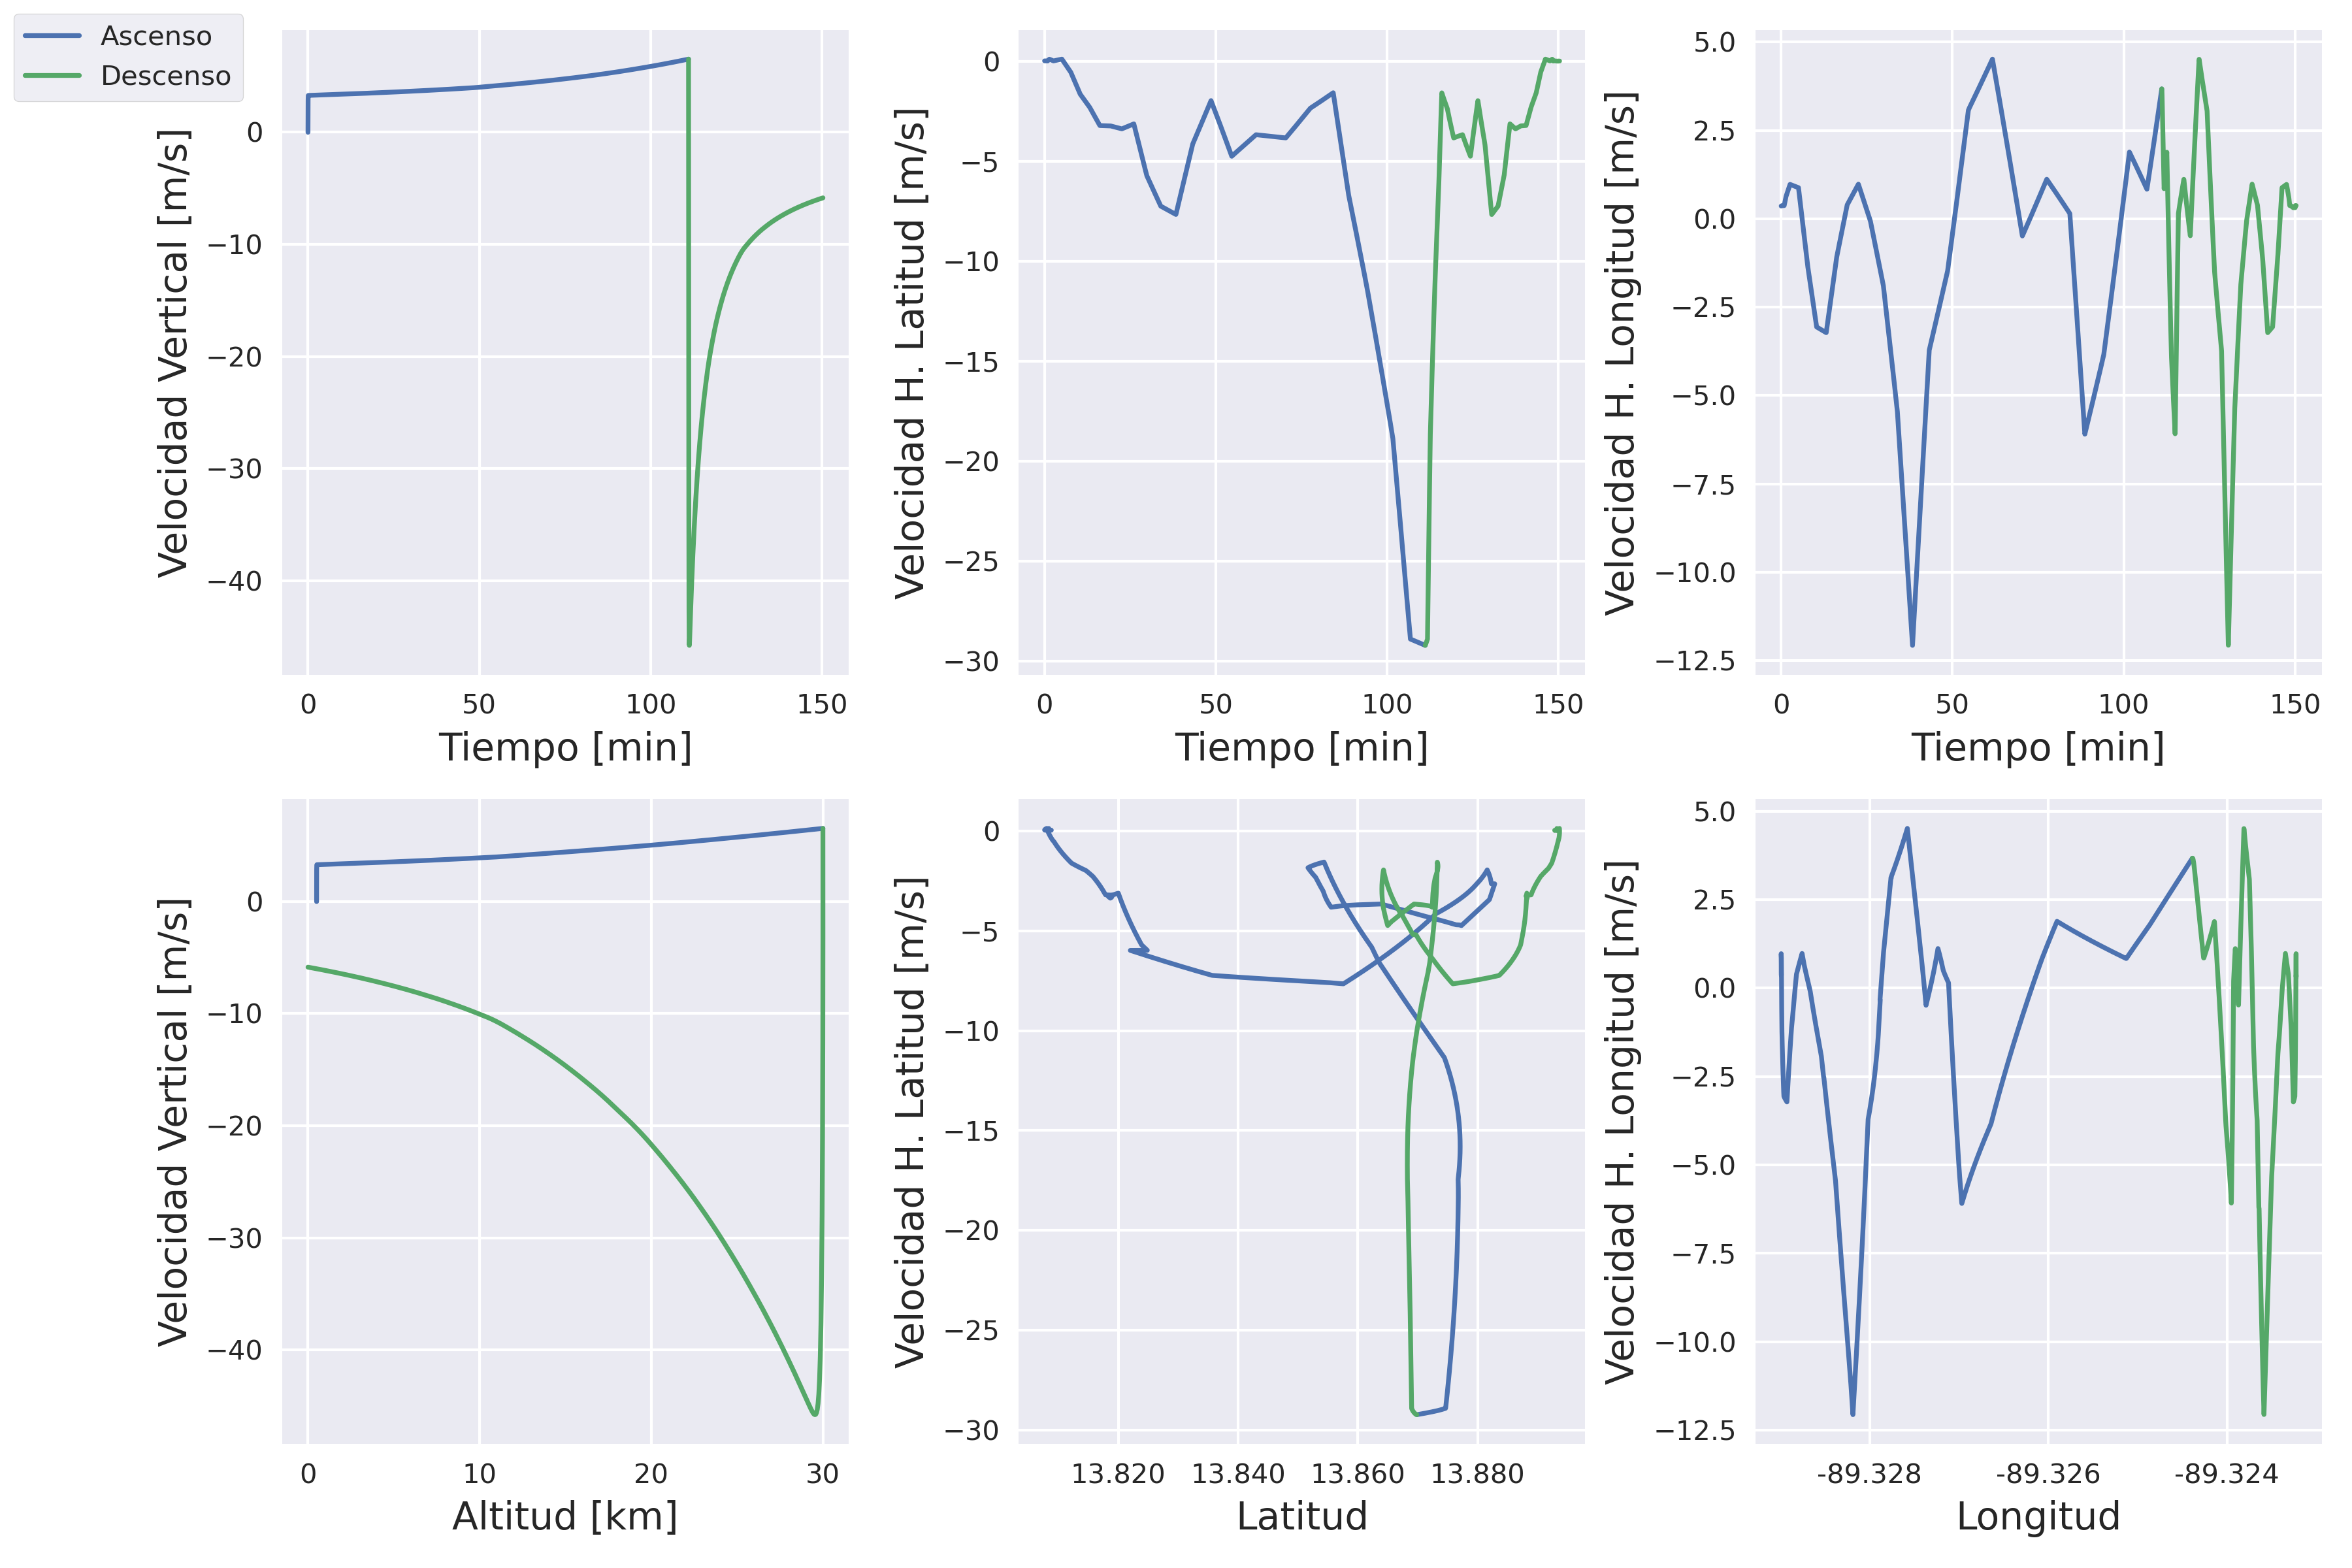
\includegraphics[width=0.77\linewidth]{document/figures/03_graficas_tiempo_altitud_vs_velocidad.png}
    \caption{Gráficas de velocidades vs posición y tiempo}
    \label{fig:velocidades_posicon_y_tiempo}
\end{figure}

\small
En figura \ref{fig:velocidades_posicon_y_tiempo} se visualiza  tres tipos de velocidades, una vertical y dos horizontales que representan la altitud, latitud y longitud. Se expone los resultados obtenidos divididos en las dos componentes del movimiento vertical y horizontal:

\begin{itemize}
    \item \textbf{Velocidad vertical respecto al tiempo y posición:}     
        \begin{itemize}
            \item En las gráficas  existe un comportamiento de aumento gradual y también bastante asintótico tanto en el tiempo como en altitud en el momento del asenso y como si se tratase de acercarse a un valor límite sin llegar a alcanzarlo, y tal como sugirió el análisis descriptivo de un promedio de 4.4 m/s con una desviación típica con baja variabilidad de 0.90 m/s. El descenso muestra una desaceleración como si de un logaritmo inverso se tratase, y se observa que el objeto al momento de impactar con la superficie de la tierra en la colisión presenta una rapidez  de  $- \;  5.9$  m/s, esto es efecto del paracaídas principalmente y la densidad atmosférica. Es notable, la velocidad luego de la explosión es dramática, pero es un comportamiento normal de un sistema bajo los efectos de caída libre que no parte del reposo.
        \end{itemize}

    \item \textbf{Velocidad horizontal en latitud y longitud respecto al tiempo y posición:}
    \begin{itemize}         
        \item A medida que el tiempo y la posición avanza, el globo se desplaza con ciertas velocidades a lo largo de diferentes latitudes y longitudes, lo cual se refleja en la variación en las gráficas que presentan fluctuaciones y oscilaciones. 
        \item Se observó que existencia tendencias anormales en el que las velocidades con respecto al tiempo y la posición geográfica sugiere un comportamiento simétrico cuando debería existir más aleatoriedad. Esta información recuerda a la poca variación que mostró en el análisis descriptivo.  
    \end{itemize}

\end{itemize}
\normalsize

\newpage

\subsection{Geometría del globo vs posición y tiempo}

Conforme en ecuación \ref{eq:radio} se realizaron los cálculos para ver como este fenómeno evoluciona en función del tiempo y la altura. 

\begin{figure}[H]
    \centering
    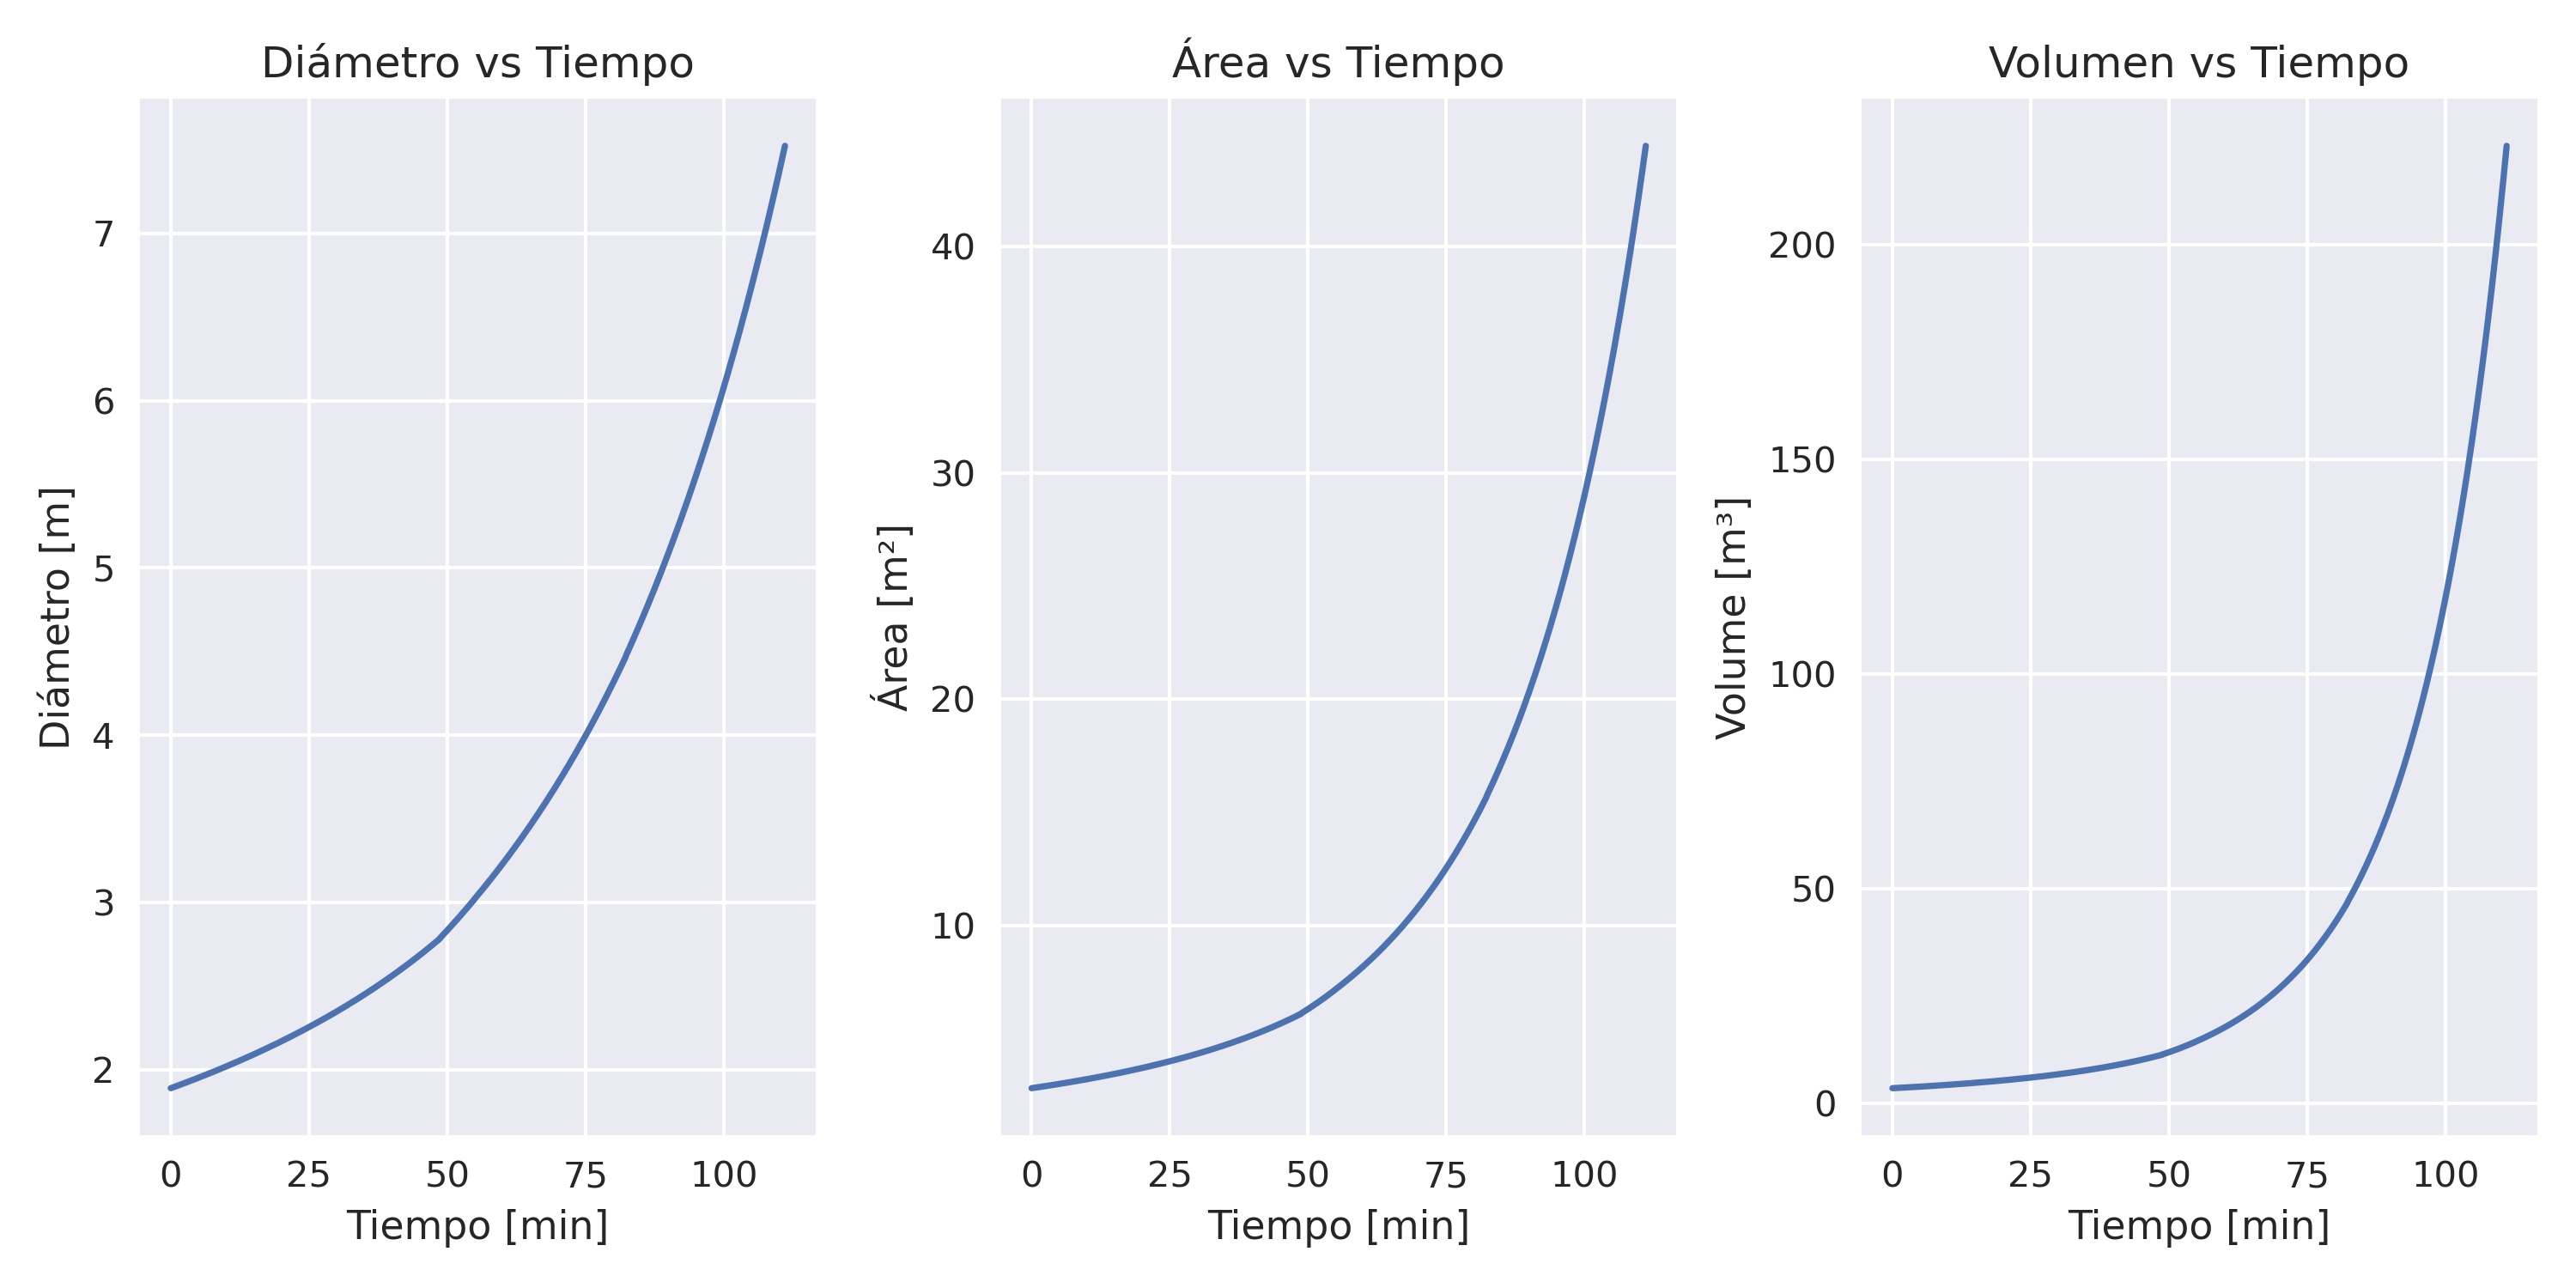
\includegraphics[width=0.9\linewidth]{document/figures/03_geometria_vs_tiempo.png}
    \caption{Geometría en función del tiempo}
    \label{fig:geometria_vs_tiempo}
\end{figure}

\begin{figure}[H]
    \centering
    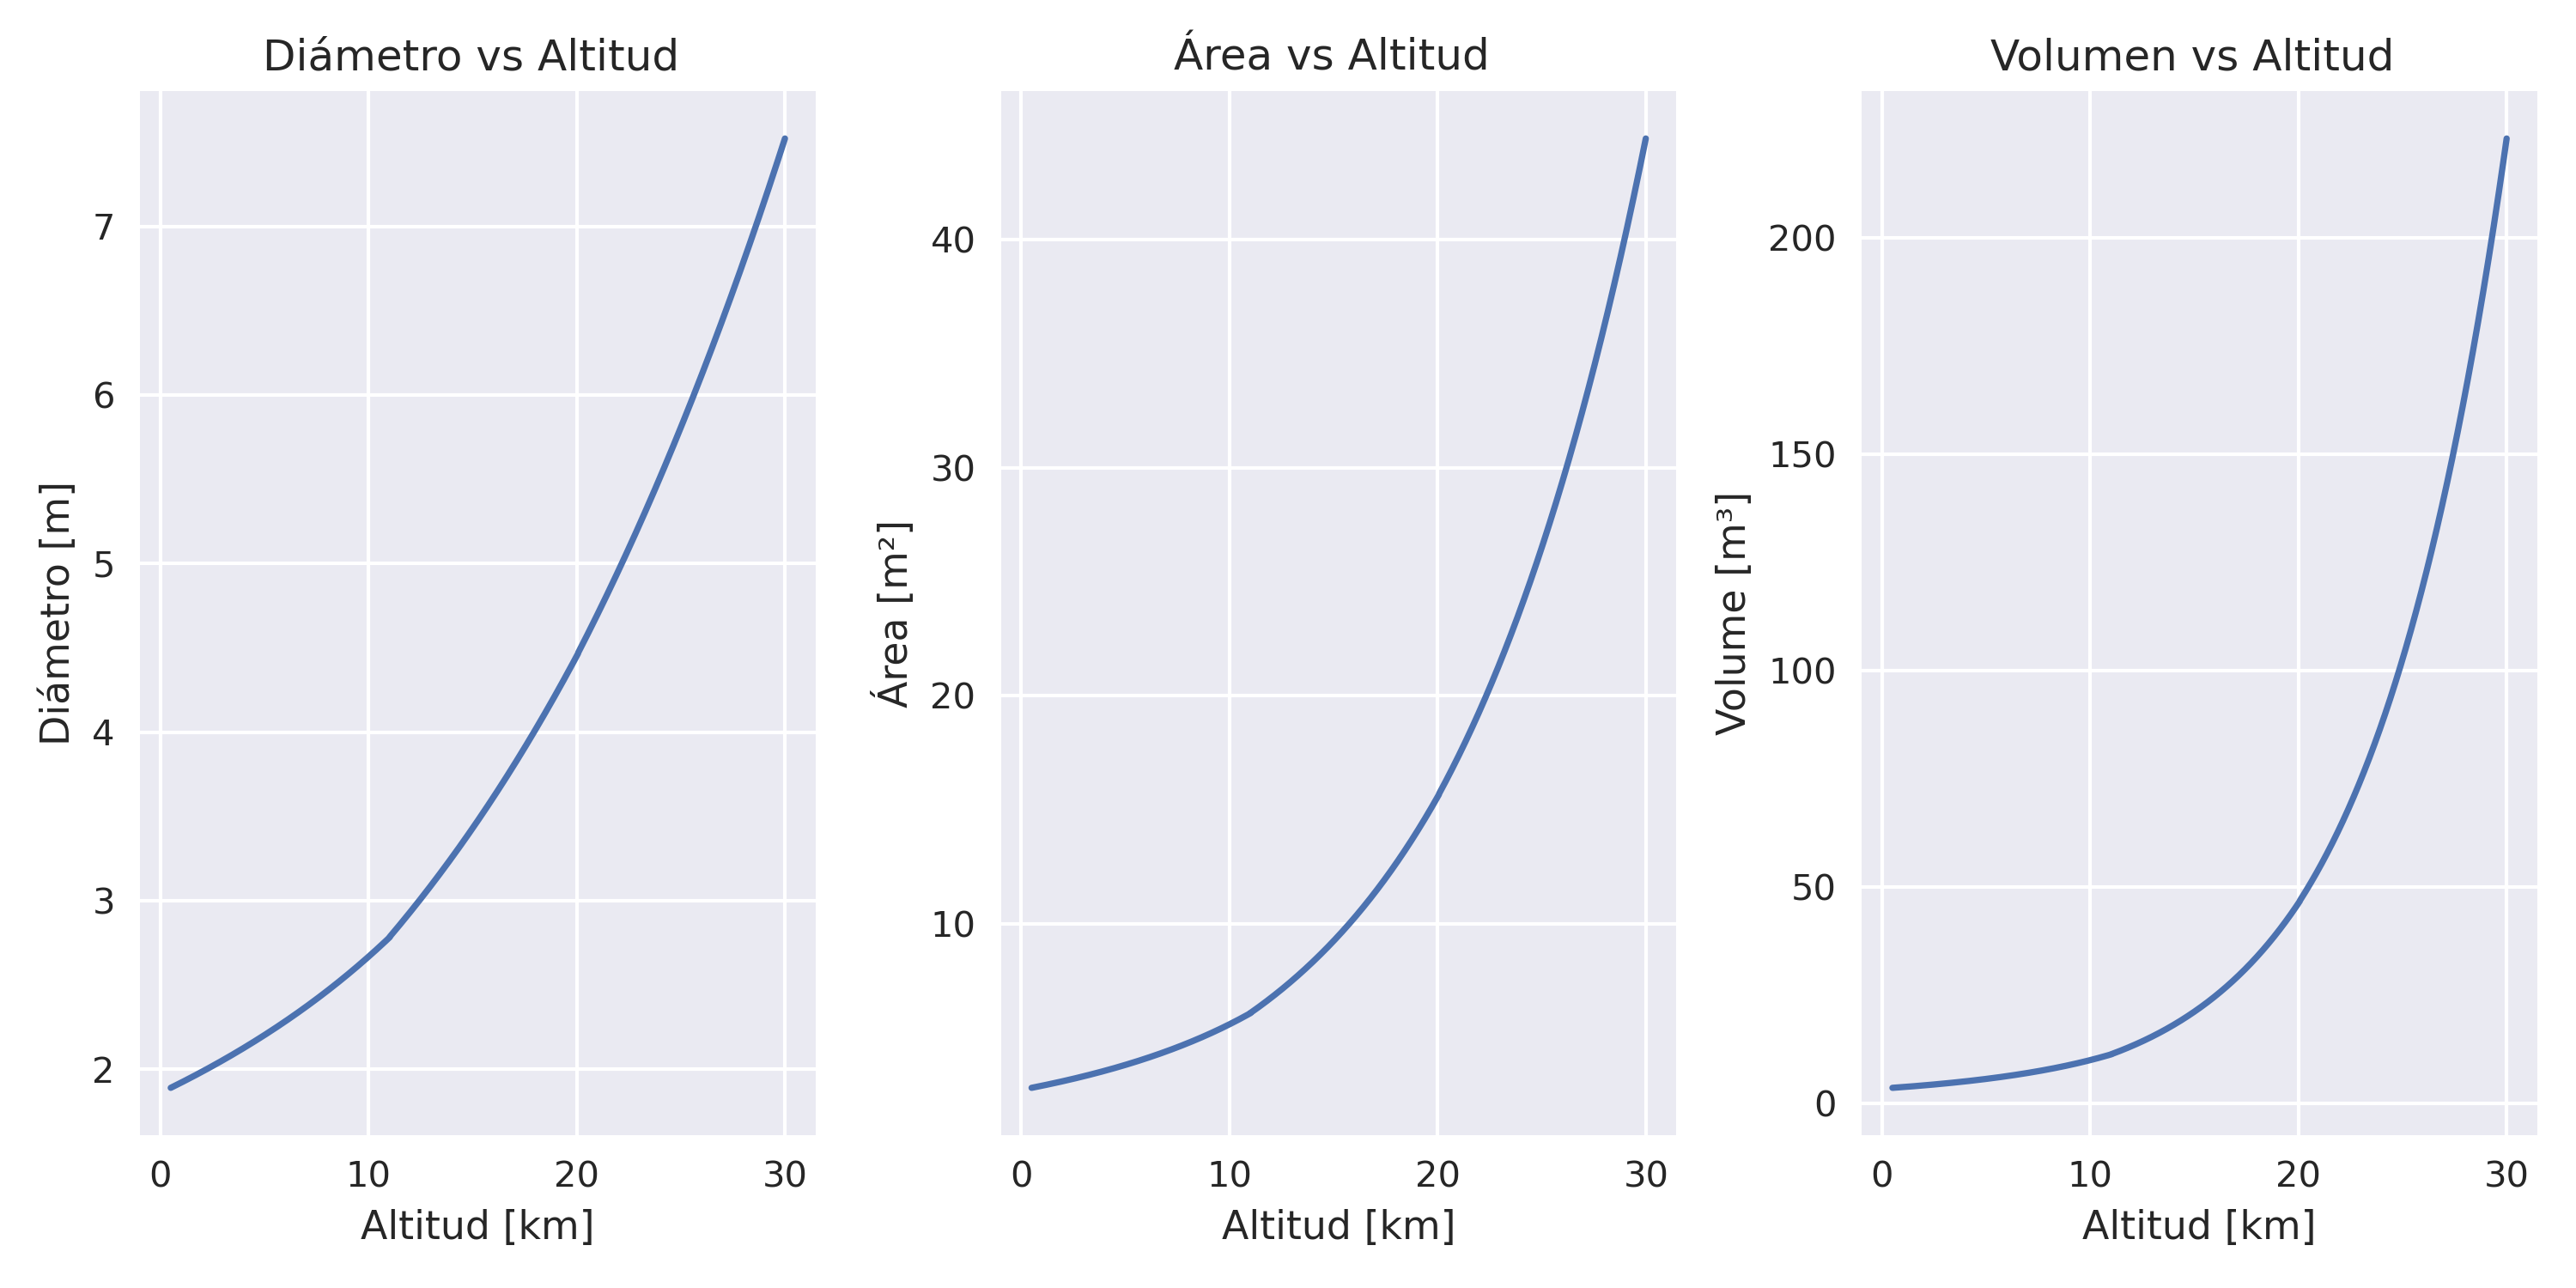
\includegraphics[width=0.92\linewidth]{document/figures/03_geometria_vs_altitud.png}
    \caption{Geometría en función de la altitud}
    \label{fig:geometria_vs_altitud}
\end{figure}

\newpage

Los resultados obtenidos en figura \ref{fig:geometria_vs_tiempo} y \ref{fig:geometria_vs_altitud}  modelan que el globo aproximadamente cambian su geometría bruscamente  después de los 12 km y 50 min, crecimiento más aceleradamente partir de ese momento. Generalmente, todas las gráficas tiene una forma exponencial, la razón de este comportamiento es que el área y el volumen depende del diámetro de globo y este último a su vez depende de las condiciones atmosféricas presentes en diferentes altitudes que cambia al transcurso del tiempo.

\begin{figure}[h]
    \centering
    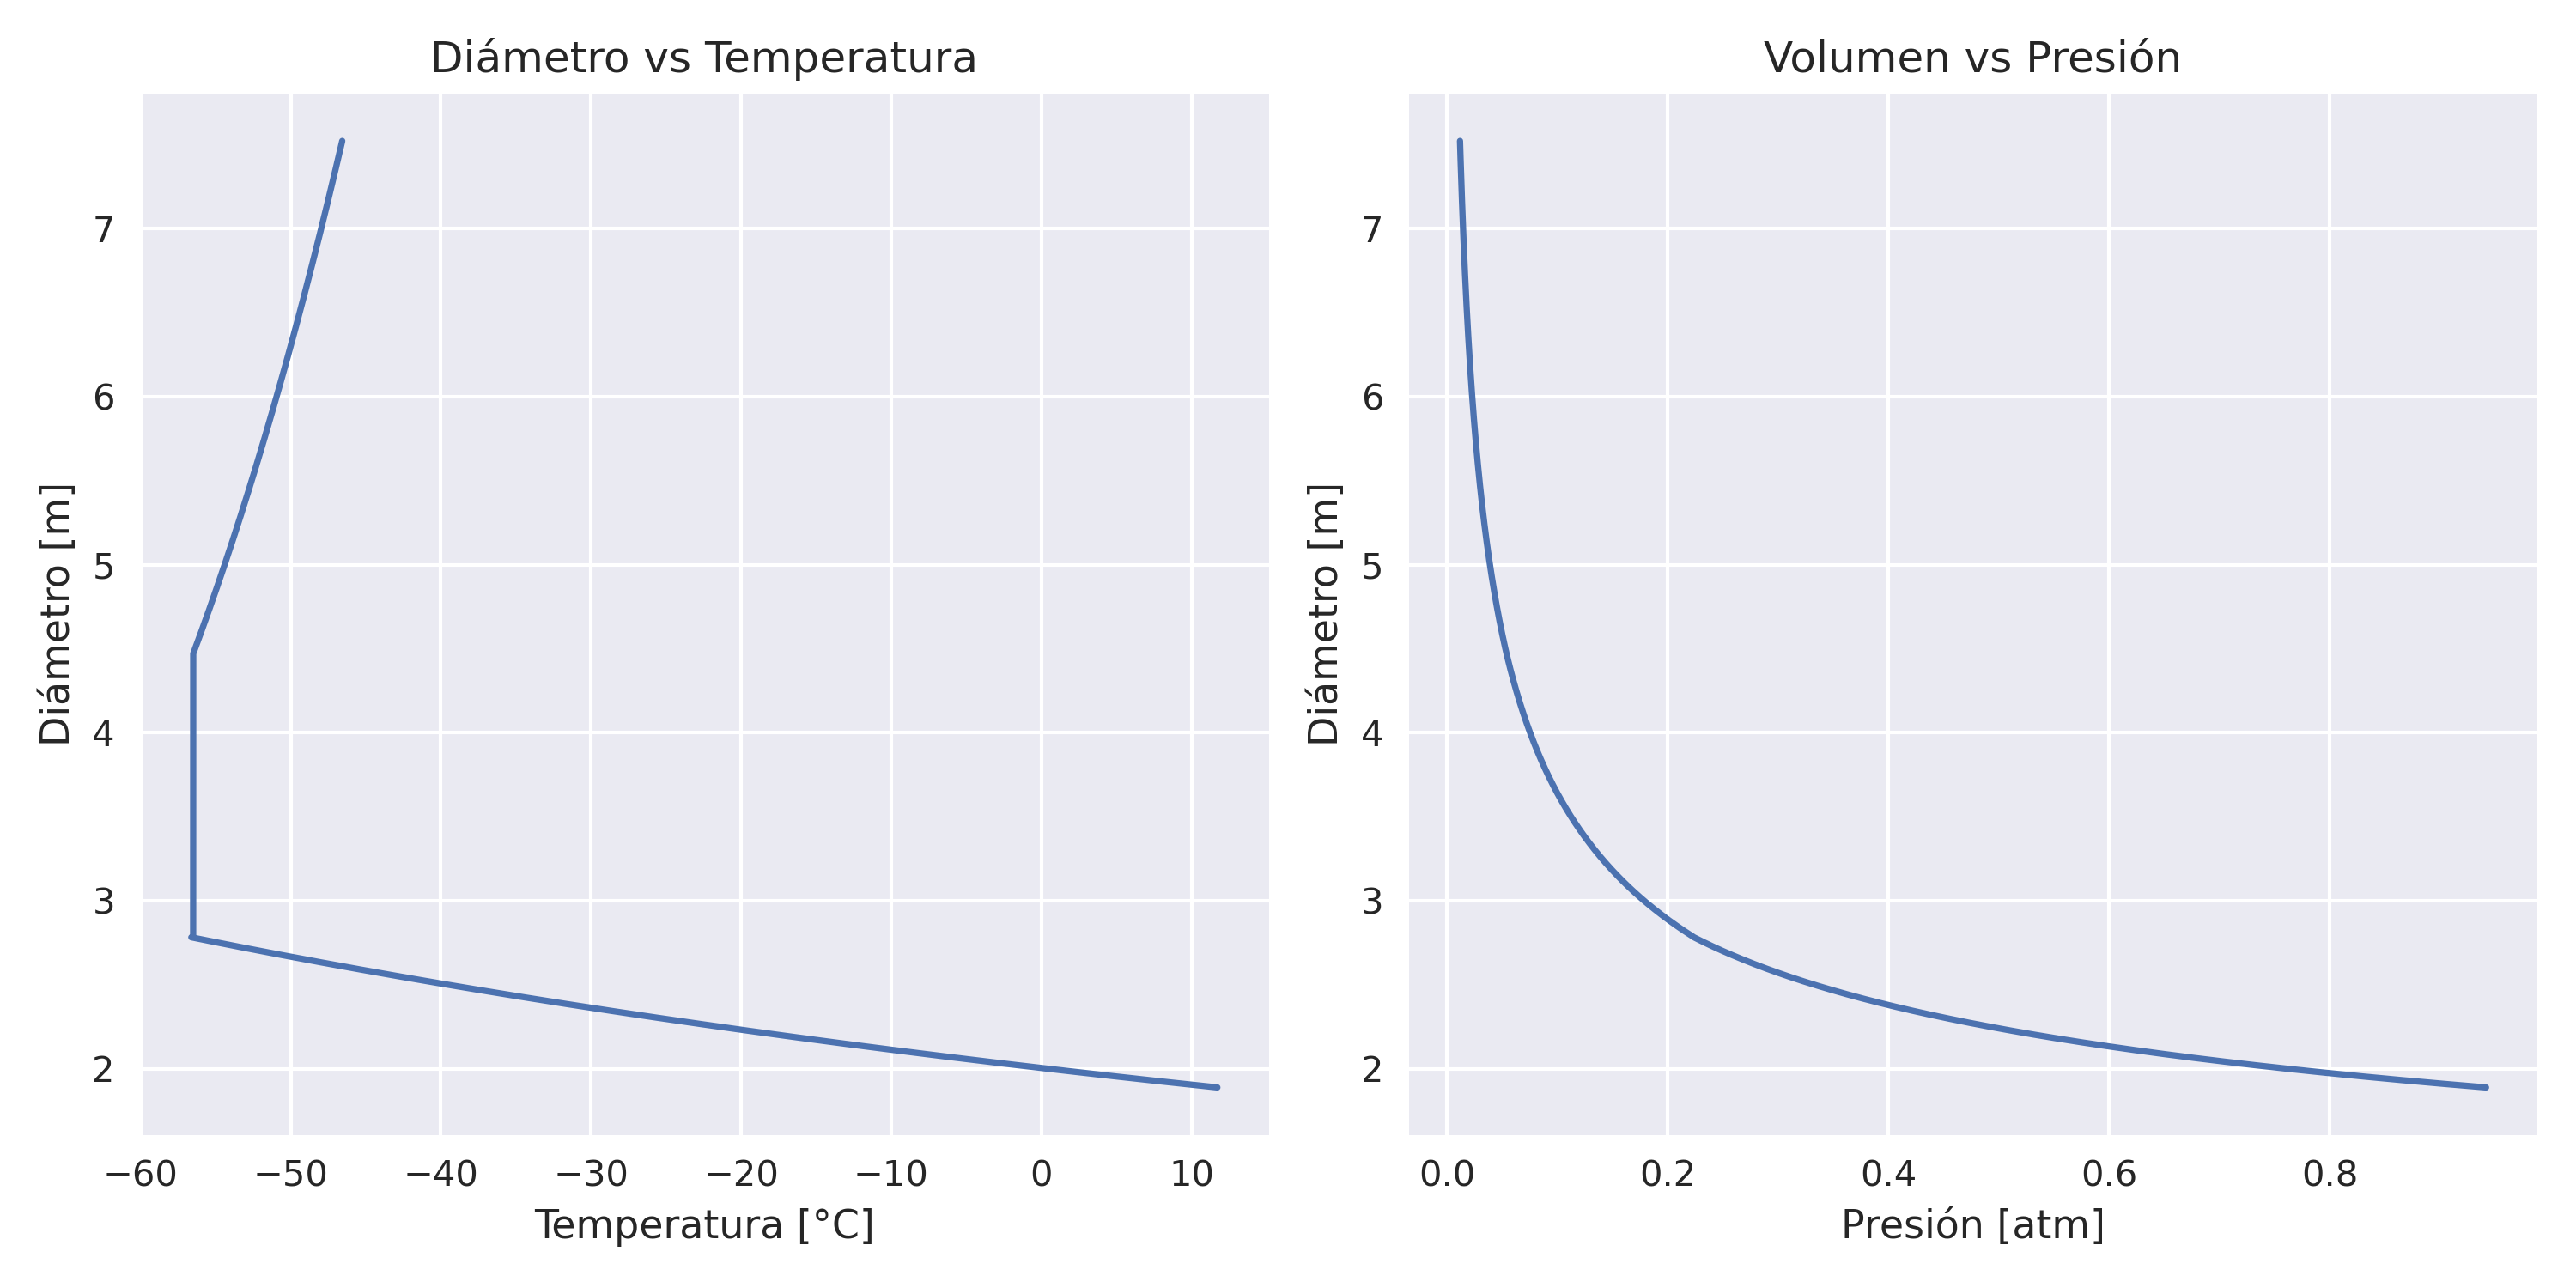
\includegraphics[width=1\linewidth]{document/figures/03_geometria_vs_atmosfera.png}
    \caption{Geometría en función del tiempo}
    \label{fig:geometria_vs_atmosferica}
\end{figure}

Cuando se analiza el diámetro en función de las variables atmosféricas presentes de la ecuación \ref{eq:radio}  como se muestra en la figura \ref{fig:geometria_vs_atmosferica} observamos que la temperatura no es tan significativa en el aporte al crecimiento del diámetro a diferencia de la caída de presión al ascender en la atmósfera quién es la causante de la explosión del globo, por lo tanto,  cuando se estime la cantidad del gas de elevación se debe de tener espacial cuidado en la cantidad  de gas porque determinará la altitud máxima debido a la presión.

La altitud y longitud no presenta ninguna relación con la geometría, esa es la razón por la que no existe ninguna gráfica con respecto a estas variables ni de las demás del conjunto de datos.

\newpage

\subsection{Atmosféricos vs posición y tiempo}

Al analizar los resultados de figura \ref{fig:atmosferica_altitud}, se observa que la relación entre la temperatura y la altitud presenta un comportamiento lineal seccionado. El primer tramo muestra una pendiente de  -6.5 °C/km, la cual está altamente influenciada por la transferencia de calor por convección, lo que sugiere que es el tramo donde los componentes electrónicos estarán bajo el mayor estrés térmico \cite{TASEC_Lab}. Posteriormente, se alcanza una región intermedia isotérmica entre los  11 km y 20 km y luego se produce un tramo final con una pendiente de +2.8 °C/km hasta llegar a los 30 km\footnote{Recuérdese, que los delta de temperatura de Kelvin y Celsius son directos}. Estas condiciones son críticas para cualquier sistema electrónico involucrado y la estructura de la sonda.

Continuando con figura \ref{fig:atmosferica_altitud},  en la presión y densidad, se puede apreciar un comportamiento exponencial en decadencia, teniendo en el caso de la densidad valores límite de 0.01845 kg/m³, para la presión 0.000118431 atm (12 hPa). Por último, la gravedad varía de forma lineal inversamente proporcional a la altura con una pendiente de --0.003056 $\frac{m}{s^{2}}$/$km$ .

\begin{figure}[h]
    \centering
    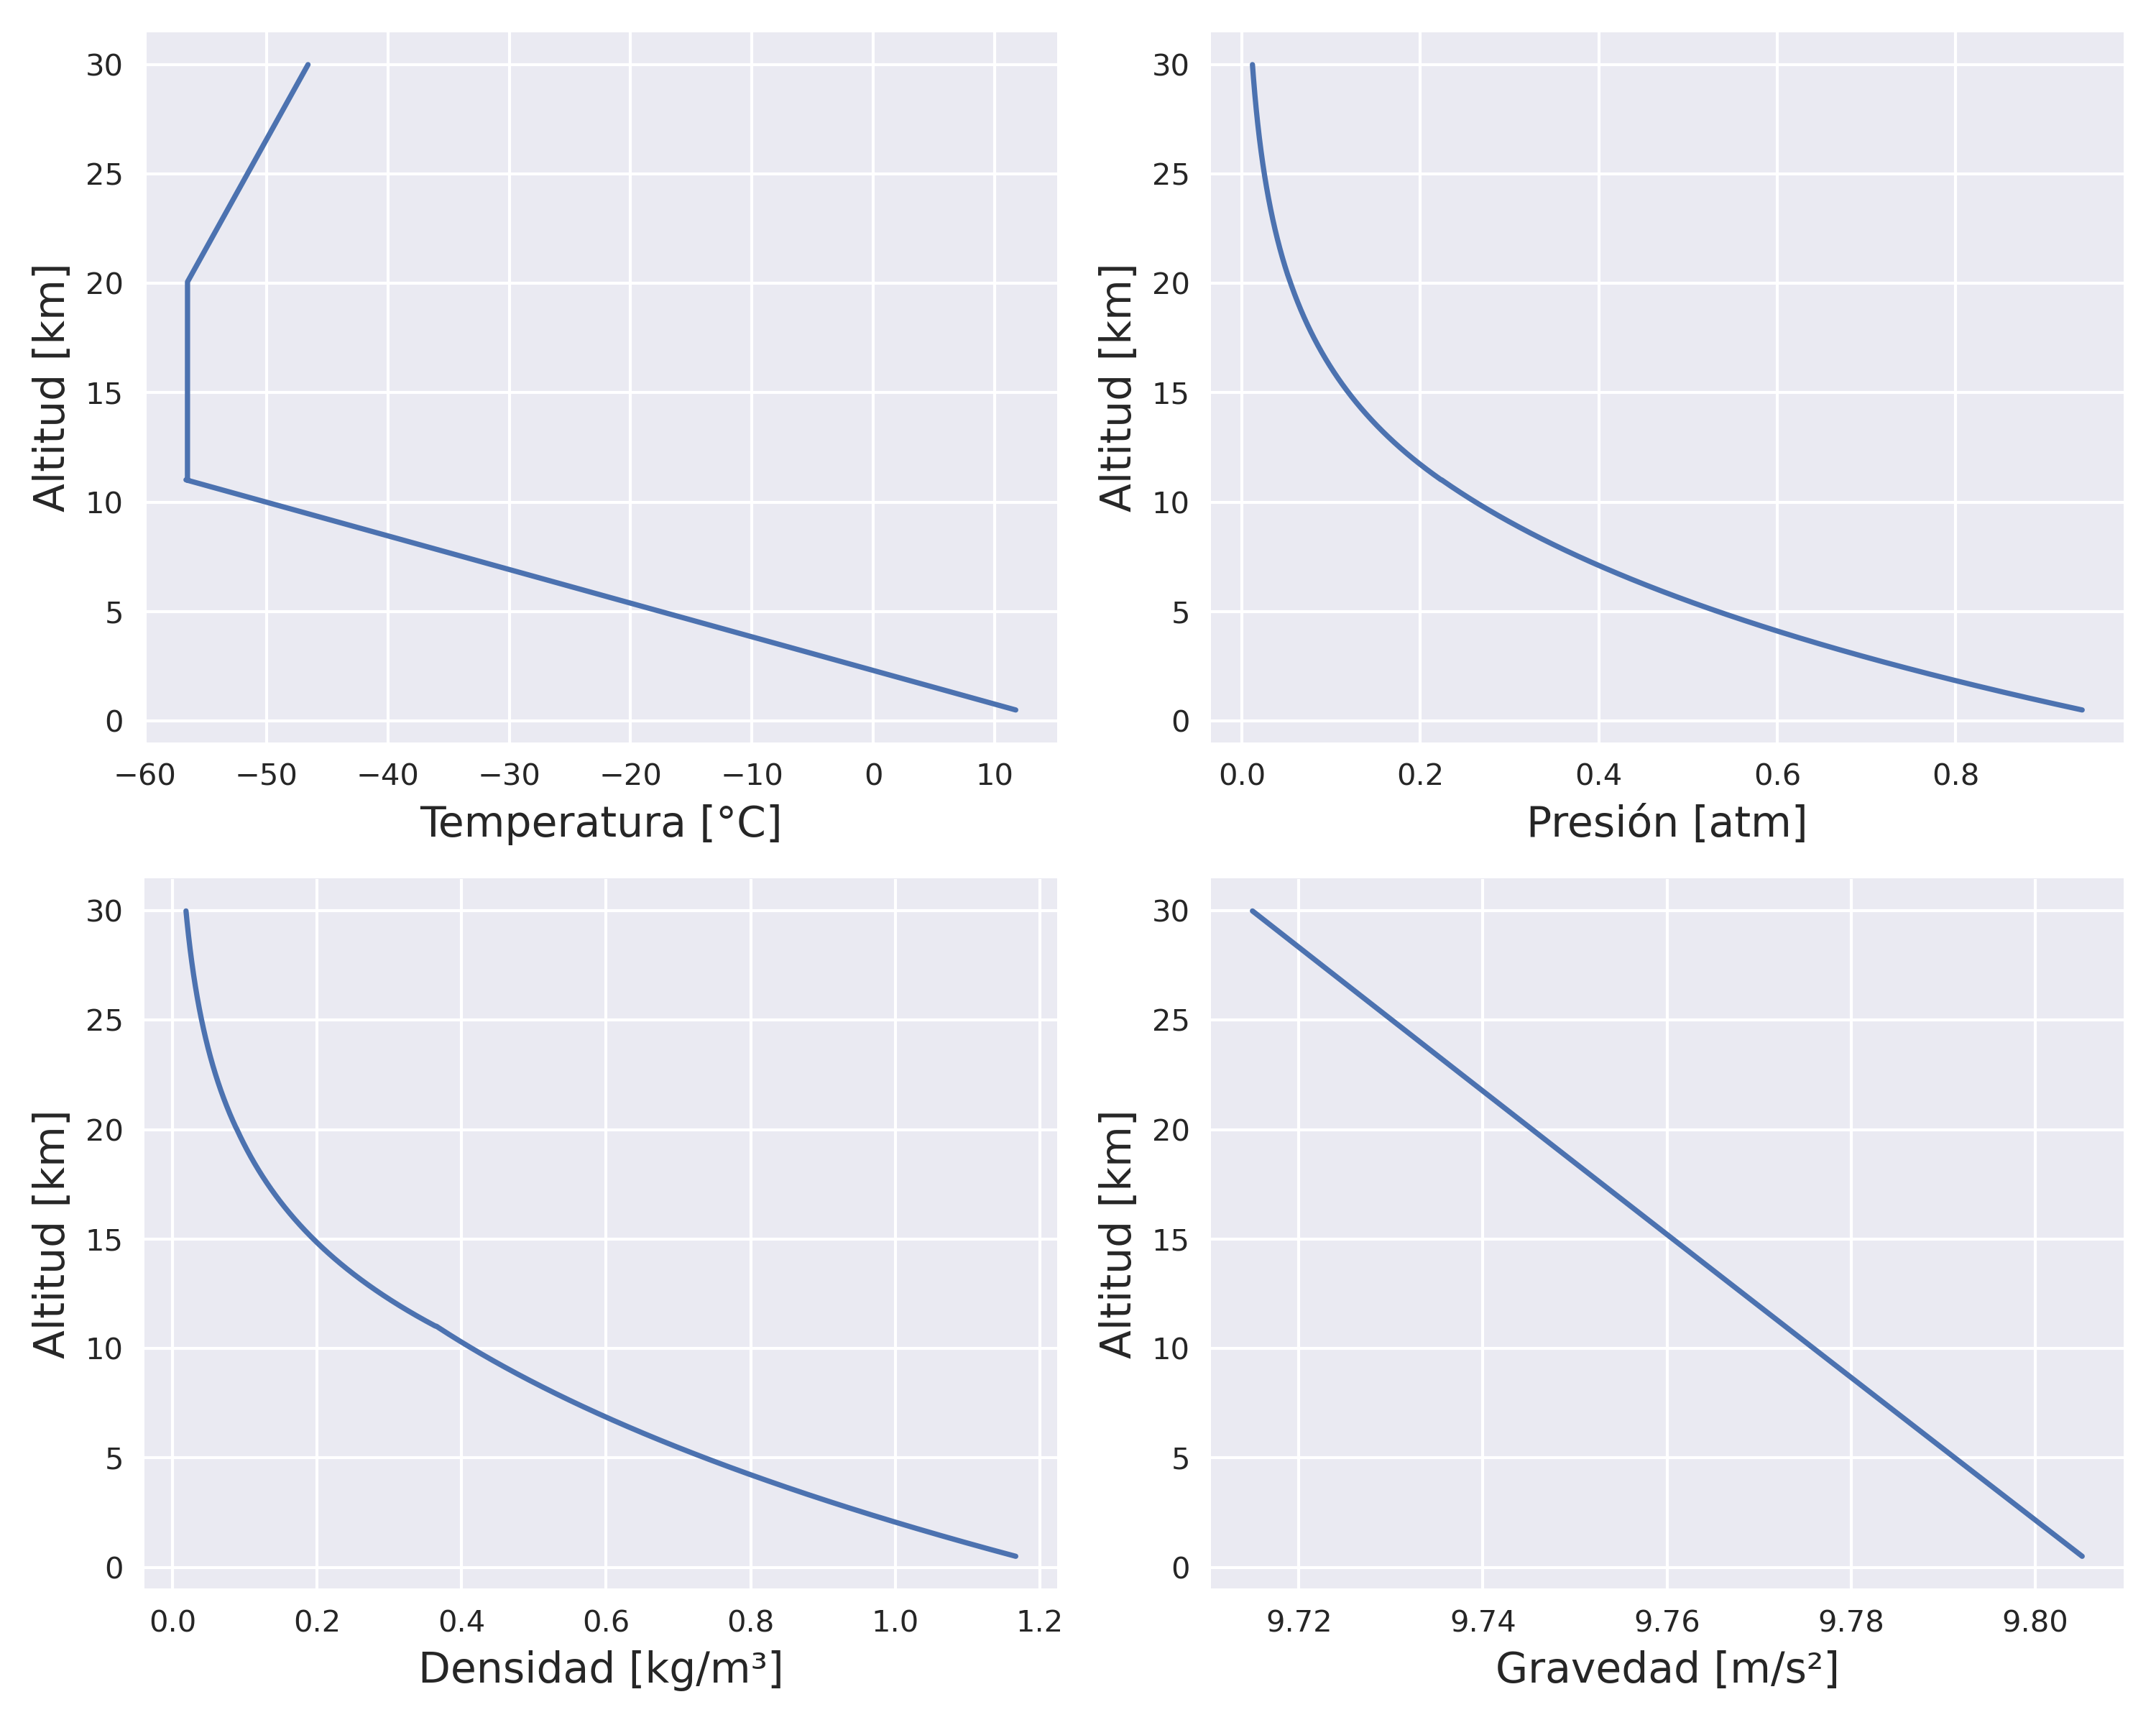
\includegraphics[width=0.85\linewidth]{document/figures/03_atmsferica_vs_altitud.png}
    \caption{Variables atmosféricas respecto a la altitud}
    \label{fig:atmosferica_altitud}
\end{figure}

\newpage

\begin{figure}[!t]
    \centering
    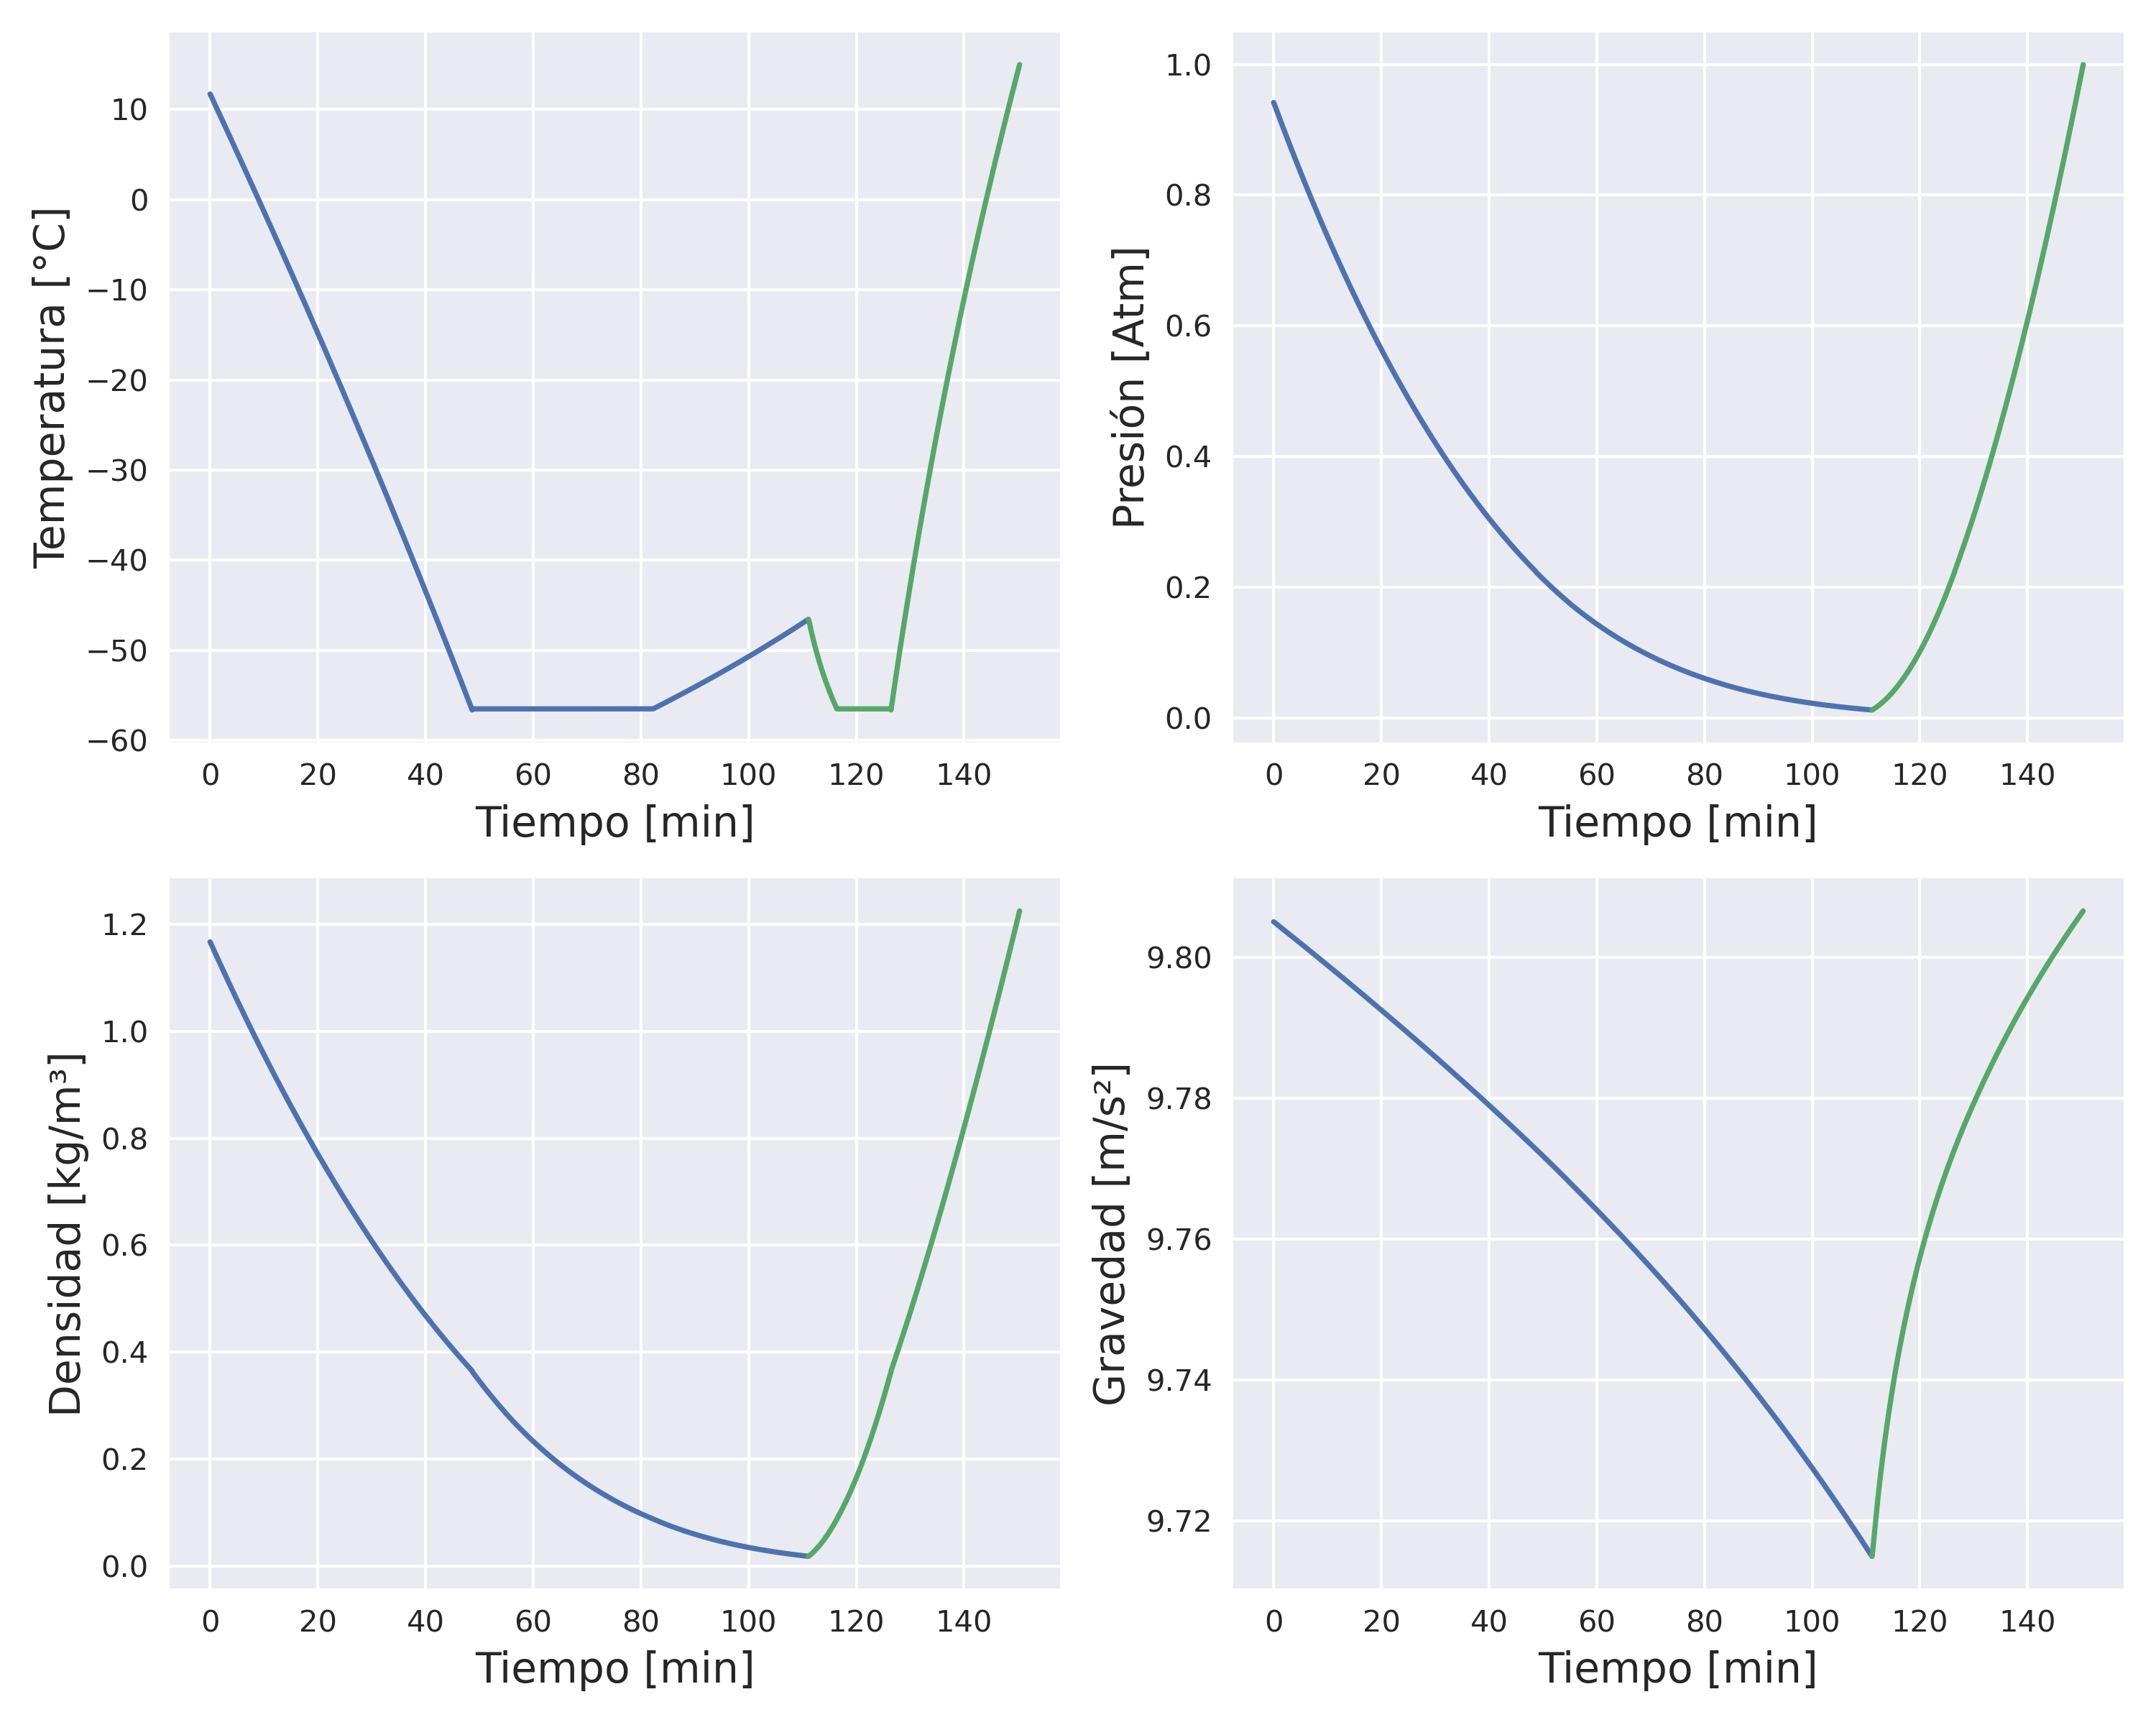
\includegraphics[width=0.75\linewidth]{document/figures/03_atmsferica_vs_tiempo.png}
    \caption{Variables atmosféricas respecto al tiempo}
    \label{fig:atmosferica_tiempo}
\end{figure}

Una vez que se relaciona el tiempo con cada variable atmosférico, como en figura \ref{fig:atmosferica_tiempo}, es posible discernir claramente las condiciones de riesgo asociadas a las tasas de cambio bruscas, especialmente en el caso de la temperatura y la presión, las cuales son las que podrían afectar a los materiales y/o componentes electrónicos en la misión.

Al analizar la curva de temperatura en función del tiempo, se puede determinar la tasa de cambio en ascenso de $-1.4$ °C/min entre 0 min y 49 min, así como otra tasa de cambio de $+0.4$ °C/min entre 83 min y 111 min. Por otro lado, en ascenso existe una disminución de $-1.63$ °C/min entre 111 min y 117 min, así para el aterrizaje se tiene $+2.2$ °C/min entre 117 minutos y los 150 minutos. De manera similar, al examinar la curva de presión en función del tiempo, se puede identificar la tasa mínima de cambio de $-0.009$ atm/min si se analiza de forma lineal entre 0.0 min y 111 min, así como la tasa máxima de cambio de $0.03$ atm/min entre 111 min y 150 min. Todo lo anterior indica las condiciones y de qué forma cambia cualquier sistema que desarrolle la trayectoria como la que describen la simulación, a partir de esto es que se desarrolla el dimensionamiento del capítulo 4.




\newpage

\section{Reflexiones y apreciaciones}


Se planteó el objetivo de desarrollar un análisis exploratorio de los datos del simulador  que se consideraron fundamentales para comprender la trayectoria del globo sonda para obtener una visión general para proceder a dimensionar el subsistema de navegación. Como resultado de lo anterior,  a continuación se presentan de los principales hallazgos de este capítulo:

\textbf{a) Presión y temperatura críticas:}

Los resultados revelaron que tanto la presión como la temperatura son factores críticos en el comportamiento de la trayectoria del globo sonda. La disminución de la presión emergió como un riesgo significativo, ya que provoca la explosión del globo. Asimismo, se identificó la importancia de controlar y monitorear la temperatura en el sistema para evitar complicaciones durante el ascenso y descenso.

Es importante tener en cuenta que estos cambios en los parámetros físicos serán críticos para el diseño de misión, especialmente si se tiene en cuenta la tercera variable crucial: el tiempo. 

\textbf{b) Velocidad del viento:}

Contrario a las expectativas iniciales de aleatoriedad en los vientos, se encontró que la implementación incorrecta en el código de simulación afectó los resultados relacionados con la velocidad del viento. A pesar,  que los cambios de los  vientos pueden estar influenciados por los patrones atmosféricos regionales y fenómenos locales, como sistemas de alta y baja presión, no fue lo observado en el trayecto como se ve en figura \ref{fig:vientos}. Estos hallazgos resaltan la necesidad de una rigurosa validación del código y un enfoque más preciso para modelar la variabilidad de los vientos en futuros estudios.  


\textbf{c) Variación de la gravedad:}

Se observó que la gravedad muestra una variación mínima en la trayectoria del globo sonda. Este hallazgo sugiere que la influencia gravitacional se mantiene relativamente constante durante el ascenso y descenso, lo cual puede tener implicaciones importantes en futuras misiones similares.

\textbf{d) Duración del ascenso y descenso:}

Se determinó que el tiempo de ascenso representa aproximadamente el 75\% del tiempo total, mientras que el descenso comprende aproximadamente el 25\% restante. Esta relación temporal asimétrica tiene implicaciones prácticas para la planificación y el diseño de misiones de globo sonda, y podría influir en la toma de decisiones relacionadas con el muestreo y la recopilación de datos en diferentes fases de la trayectoria.
%  Se me fue lo de la la gravedad 
En resumen, este estudio exploratorio y de estadística descriptiva proporciona una comprensión más profunda de la trayectoria ascendente y descendente de un globo sonda. Los hallazgos destacan la validación correctamente del modelo de velocidad del viento, monitorear la presión y la temperatura crítica, y tener en cuenta la asimetría temporal en el tiempo de ascenso y descenso. Estos resultados pueden servir como base para futuras investigaciones y mejoras en el diseño y ejecución de misiones de globos sonda.

\begin{figure}[h]
    \centering
    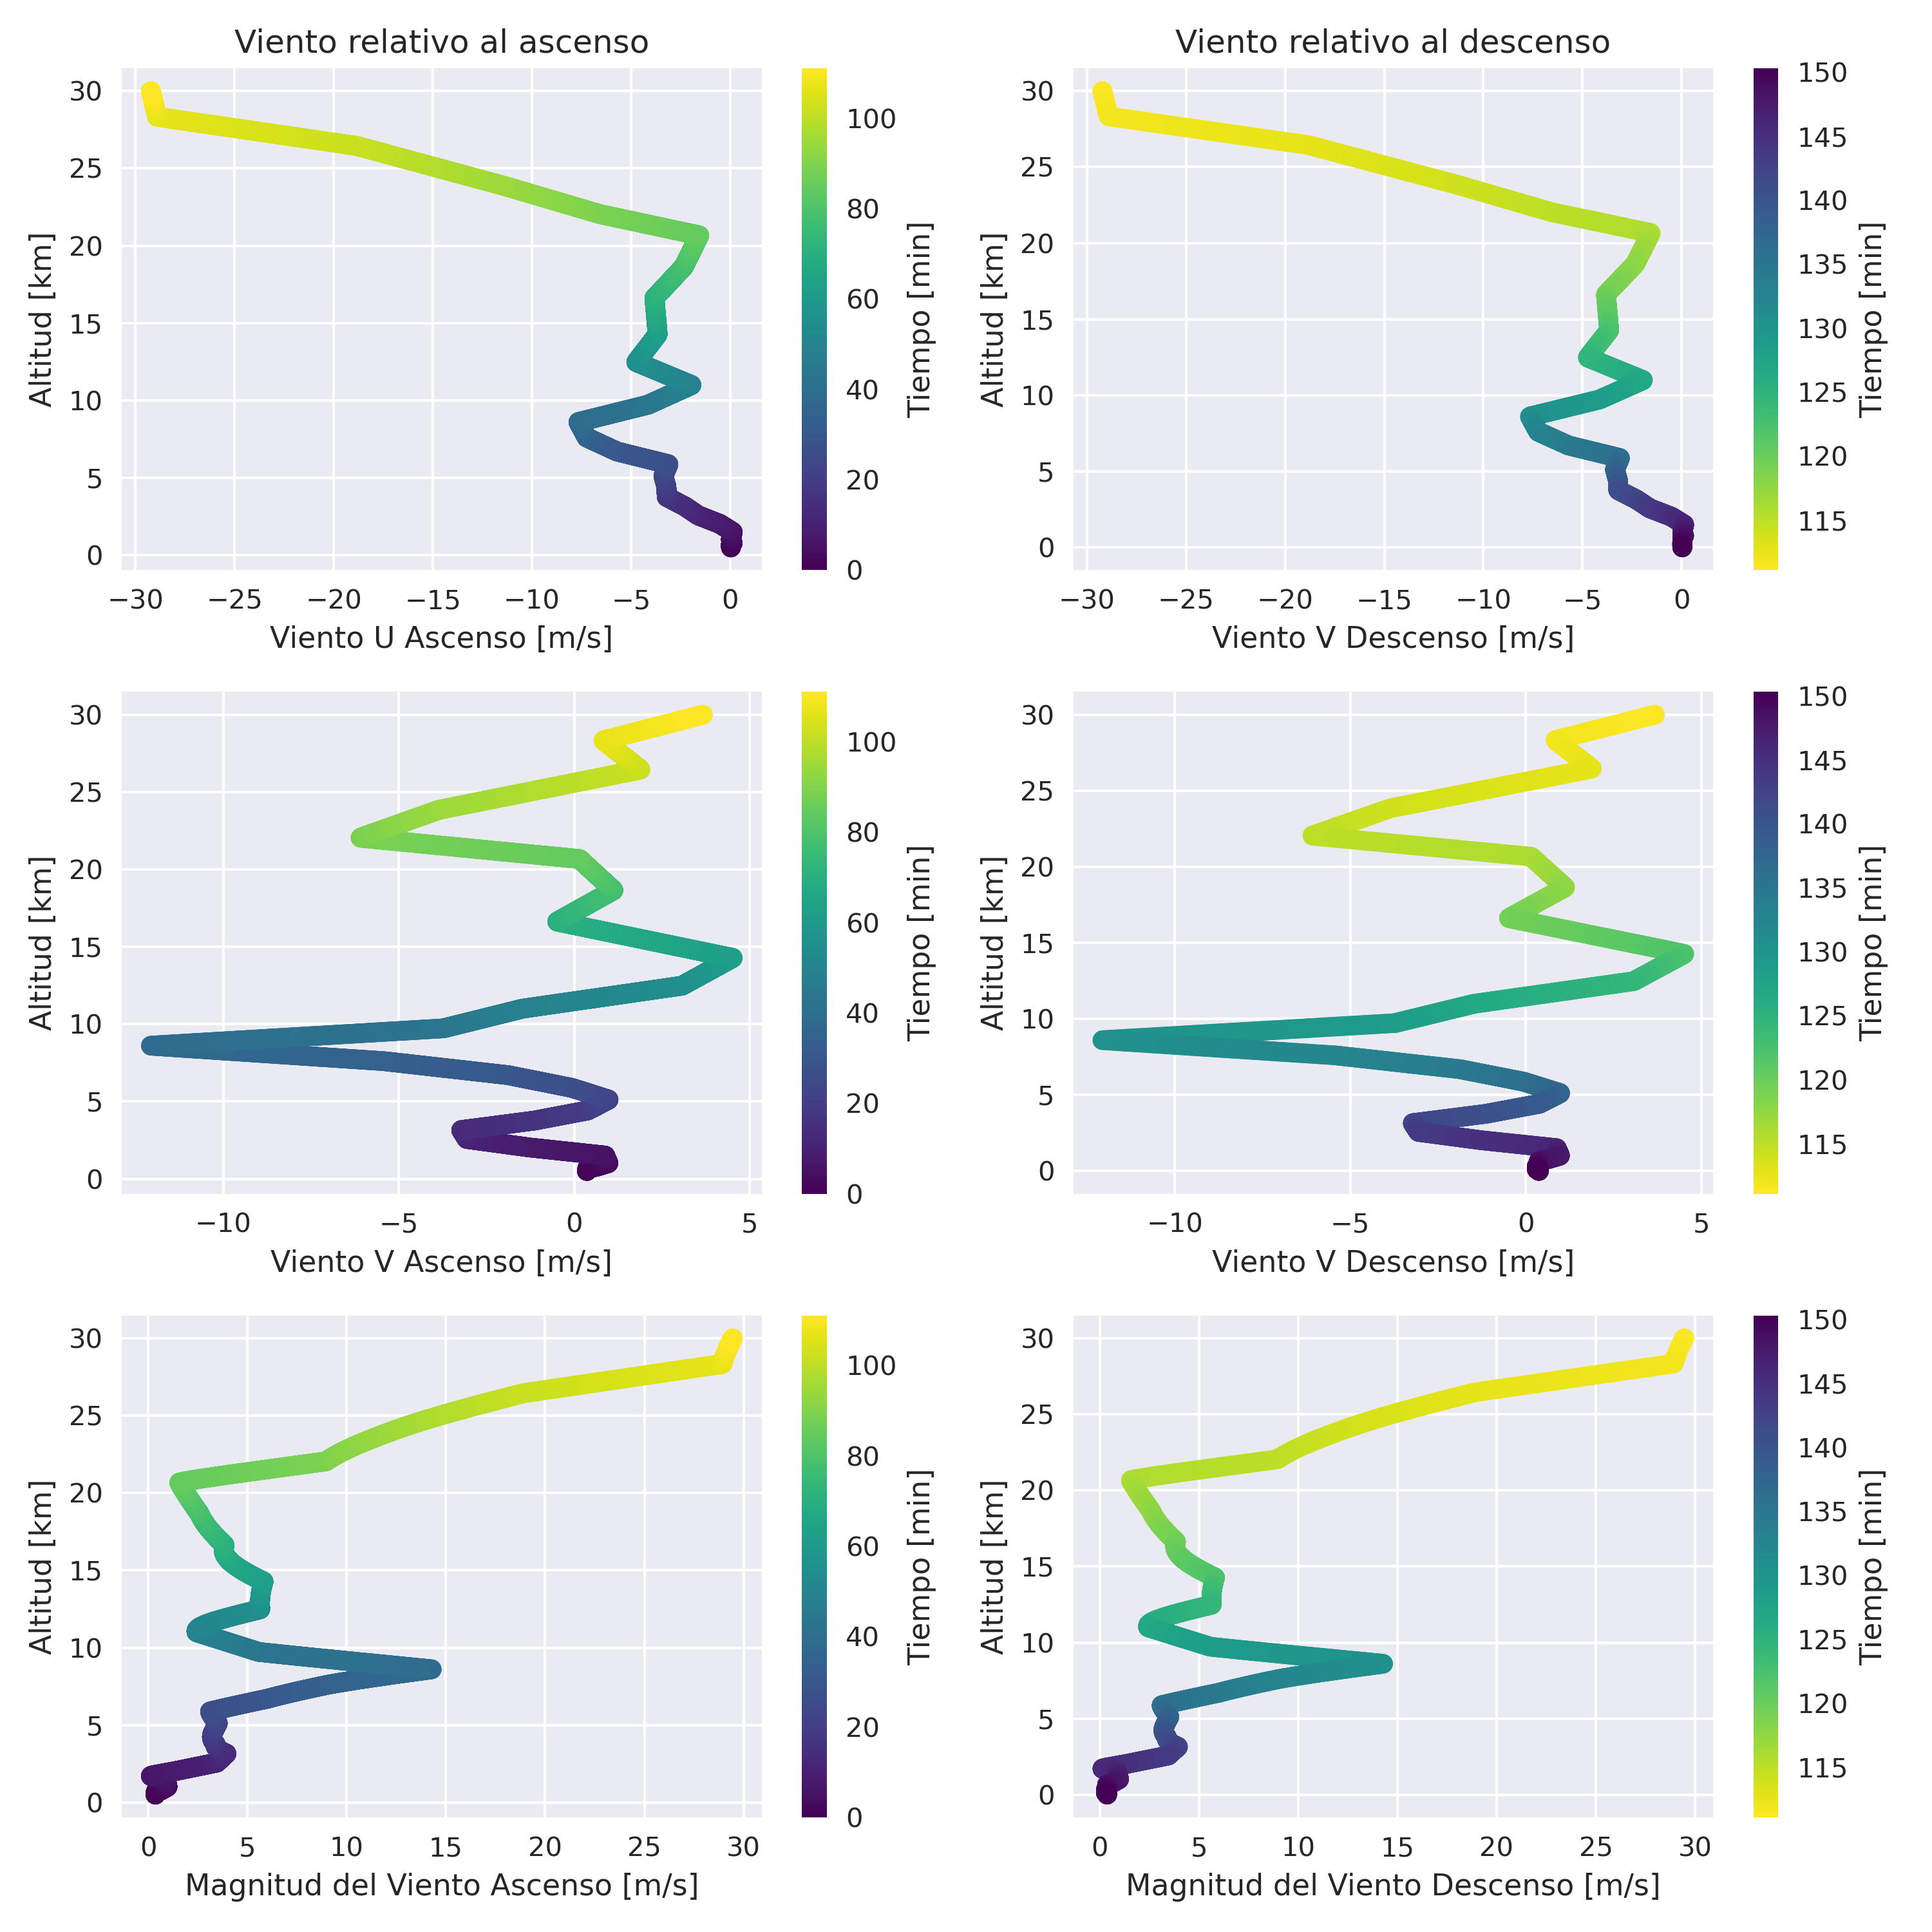
\includegraphics[width=0.85\linewidth]{document/figures/03_vientos.png}
    \caption{Vientos en diferentes planos}
    \label{fig:vientos}
\end{figure}
\chapter{Dimensionamiento de Subsistema de Navegación} \label{chp:dimensionamiento}

\vspace{0.2cm}


En este capítulo, se evalúa una opción de dimensionamiento de un subsistema de navegación que implica la estimación de componentes electrónicos necesarios, su capacidad y rendimiento requeridos para misiones near-space en HABs a partir de la perspectiva brindada del análisis exploratorio en función del tiempo de las diferentes variables estudiadas. Además, se tuvo en cuenta las restricciones técnicas y  COTS (comercial off-the-shelf) de los CubeSat  como filosofía desarrollo.

\vspace{0.7cm}

El dimensionamiento de subsistemas de navegación es un aspecto   <<ad hoc>> en este trabajo, que toma de referencias PyCubed, TASEC-Lab y propuesta abierta de comunidades de Hardware y Software.  Estas referencias provee los fundamentos de  las tecnologías de la misión estratosférica StratoBalloon con una experiencia que los respalda en aplicaciones similares.

\newpage

%%%%%%%%%%%%%%%%%%%%%%%%%%%%%%%%%%%%%%%%%%%%%%%%%%%%%%%%%%%%%%%%%%%%%%%%%%%%%%%%
%%%%%%%%%%%%%%%%%%%%%%%%%%%%%%%%%%%%%%%%%%%%%%%%%%%%%%%%%%%%%%%%%%%%%%%%%%%%%%%%

\section{Subsistema de Navegación}

La navegación en el marco de lo aeroespacial se refiere al conjunto de técnicas, procesos y sistemas utilizados para obtener la posición, velocidad y dirección de una aeronave durante su trayecto,  que se apoya de la observación aérea, terrestre y de los instrumentos de vuelo en función del tipo de aeronave el cual es altamente variado y depende de las características y requisitos específicos de cada plataforma \cite{understanding_gps, gnss}. Por ejemplo, en aeronaves convencionales (aviones comerciales, helicópteros, etc.)  se utilizan principalmente  sistemas como el sistema de navegación por satélites (GNSS, por sus siglas en inglés), sistema de navegación inercial (INS)  y radionavegación con los cuales se tiene una ubicación precisa y actualizada; no obstante, en nanosatelites compone de un sistema de nominado sistema de control de actitud (o en inglés, attitude control system abreviado ACS) con puesta por sensores y actuadores como magnetómetros, sensores de constelaciones, sensor solar \cite{attitude_componentes_nanosatelites}.  En el caso de los globos sonda, algunos elementos típicos de la navegación en aeronaves convencionales y nanosatélites pueden ser aplicables o estar ausentes debido a las características peculiares de esta plataforma.

Este dimensionamiento de subsistema de navegación se desarrolla para la misión experimental "StratoBalloon" que se consideró apropiado utilizar la filosofía CubeSat como fuente de referencia principal. Por lo anterior,  se aborda de manera \textit{ad hoc}, es decir, se desarrolla una propuesta solución buscando adaptarla y que sea funcional como primera aproximación  para obtener  información relativa del seguimiento de la trayectoria del globo sonda, así como para recopilar el dato meteorológico de temperatura. Por lo tanto, en el caso particular de StatoBalloon,  los elementos que se retoman y su utilidad en el subsistema de navegación para el globo sonda son:

\begin{enumerate}
    \item \textbf{GNSS:} determina la ubicación del globo-sonda mediante las diferentes señales de las constelaciones satelitales existentes.
    \item \textbf{Sensor inercial:} también conocidos como Inertial measuremten unit (IMU), estos sensores miden la aceleración y la velocidad angular para obtener información sobre los movimientos y cambios de dirección.
    \item \textbf{Sensor barométrico:} mide la altitud en función de la variación de la presión atmosférica. 
\end{enumerate}

\textbf{Adicionales}: un microcontrolador dedicado para el subsistema como On board computer (OBC), memoria de datos y  un sensor de temperatura. Estos elementos adicionales podrían no tener sentido en la navegación propia o podrían ser  suprimidos. Se ha obviado el hecho de tener alimentación y gestión energética en el subsistema de navegación, además de un sistema de telecomunicaciones o telemetría, y también a cualquier otro subsistema que adicione StratoBalloon.

\newpage

\section{Criterios de Selección}

Existieron dos criterios de selección de componentes electrónicos: generales y simulación. Los criterios generales se basan en una forma de como diseñar un dimensionamiento tomando como principios un rápido y amigable desarrollo de estas tecnologías; por otro lado, los criterios de simulación se toman los datos de las variables que puede llegarse a medir a lo largo de la trayectoria para estimar que necesidad se tiene de equipo a utilizar.  A continuación se detallan los criterios:

\subsection{Generales}

\begin{itemize}

    \item Uso de componentes comerciales, usando el modelo COTS (comercial off-the-shelf) típico en nanosatélites.  Esto favorece la adquisición de repuestos y la compatibilidad con otros sistemas en el futuro.
    \item Obtener componentes electrónicos, considerando cuidadosamente  la calidad, el precio, precisión ofrecidos en el mercado.

    \item Buen soporte y documentación de las tecnologías o herramientas. De esta forma, se busca que los tiempos de desarrollo sean cortos, seleccionando tecnologías que nos permita alcanzar mejores resultados de manera eficiente.
    \item Optar por una modularidad e interoperabilidad entre los componentes, así permite una mayor flexibilidad, compatibilidad e integración con respecto a la configuración y actualización de los equipos.
\end{itemize}

\subsection{Simulación}

\begin{itemize}
    \item Poseer la mejor resistencia a las condiciones ambientales adversas de la atmósfera, como podrían ser robustez a cambios de temperatura y si es posible a la humedad, a pesar de no estar considerada en la simulación. En figura \ref{fig:atmosferica_altitud} y figura \ref{fig:atmosferica_tiempo} se mostró estas condiciones  adveras, exceptuando humedad. Además, se debe de considerar el tiempo de duración de la misión, que según la simulación del capítulo \ref{chp:02_simulacion}  de 2.5 horas.
    \item Cuidar el tamaño y peso de los elementos debido a que afecta en las ecuaciones \ref{eq:ascenso} y \ref{eq:descenso} relativo a la dinámica del sistema. Además, ayuda a que en un futuro poder optimizar el espacio y minimizar el peso total del sistema.
    \item Buscar la mejor eficiencia energética  en términos de consumo debido a que el recurso energético es limitado e influenciado por las condiciones adversas del ambiente \cite{condiciones_entorno_baterias}. 

\end{itemize}

\section{Componentes del Subsistema de Navegación}
 
Los componentes analizados se seleccionaron entre aquellos disponibles en el mercado local del país, buscando aquellos que ofrezcan las mejores prestaciones posibles, luego de ello,  se analizó la disponibilidad con diferentes vendedores, tiendas  y distribuidores internacionales de componentes electrónicos investigados\footnote{Se deja de lado las empresas de manufactura debido a comúnmente subcontratan la venda de sus productos y además no vende al por menor.} se mencionan algunos de ellos: como mayorista Mouser Electronics y Digi-key; como distribuidores minoristas y compañías de hardware de código abierto como Sparkfun y Adafruit. Además, se retomó componentes de algunas investigaciones  probados en condiciones similares a las mostradas por el simulador desarrollado en este trabajo.  En anexo \ref{chp:anexo:componentes_analizados&extras} se colocan diferentes componentes analizados en este trabajo, a continuación se detalla cada componente seleccionado para el subsistema:

\begin{itemize}
    \item \textbf{NEO-M9N GPS Breakout:}  es una placa desarrollada por SparkFun siendo un módulo receptor GNSS de 92 canales que puede recibir señales de los sistemas Galileo, GPS, GLONASS,  y BeiDou lo que mejora la precisión (apróx. 1.5 metros) y reduce el tiempo de sintonización,  cuenta con un conector tipo SMA para colocar la antena de preferencia. Además, es altamente configurable con el software u-center de la compañía Suiza u-blox \footnote{Software del fabricante: \url{https://www.u-blox.com/en/product/u-center}}.  Este es el único elemento que no está presente en algún estudio, se seleccionó por su alta prestaciones y precisión al tener alta disponibilidad de constelaciones satelitales;  los datos de posición de latitud, longitud analizados en el simulador aparentemente puede tener la presión según modelos matemáticos usados y la forma de resolver los modelos, viendo la importancia de obtener los mejores datos de posición (alta disponibilidad y la mejor presión) se seleccionó este equipo, además de su alta documentación y respaldo de SparkFun. En figura \ref{fig:gnss} se muestra el módulo.

    \begin{figure} [h]
        \centering
        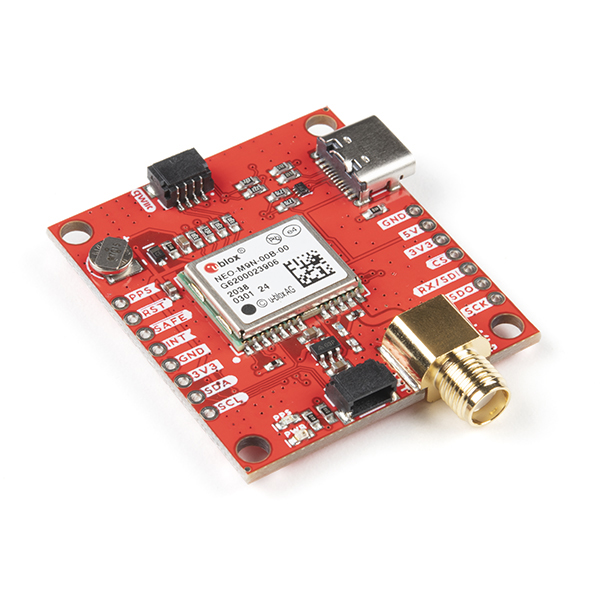
\includegraphics[width=0.25\linewidth]{document/figures/04_GPS__NEO-M9N__SMA__qwiic_sparkFun.jpg}
        \caption{GPS Breakout, Créditos a SparkFun CC BY 2.0, sin edición.}
        \label{fig:gnss}
    \end{figure}

    \item \textbf{Registro de vuelo:}  se utiliza OpenLog de Sparkfun y una tarjeta microSD SanDisk High Endurance, con los cuales se almacena y registra datos durante el vuelo,  esto permite capturar y analizar datos meteorológicos y variables del globo sonda para su posterior estudio para fines científicos o de depuración. El criterio de selección de la microSD fue dada por  \cite{sd_pycubed, pycubed}. En figura \ref{fig:openlog} y figura \ref{fig:microsd}  se muestran los dispositivos/
\begin{figure}[h]
    \centering
    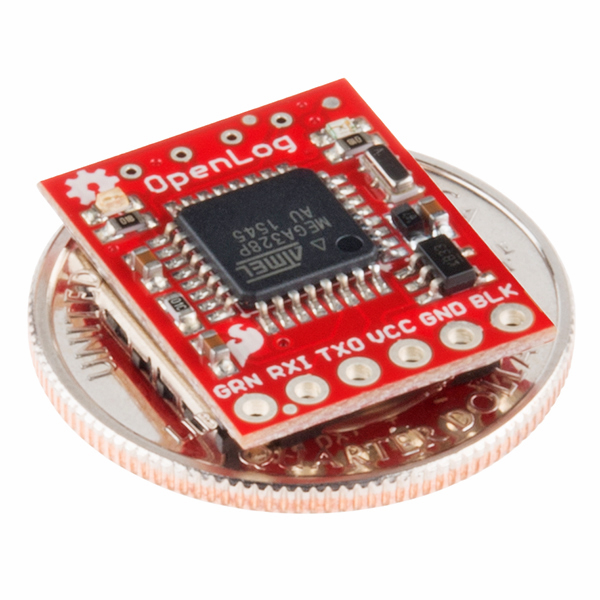
\includegraphics[width=0.25\linewidth]{document/figures/04_OpenLog_SparkFun.jpg}
    \caption{OpenLog. Créditos a SparkFun CC BY 2.0, sin imagen edición}
    \label{fig:openlog}
\end{figure}

\begin{figure}[h]
    \centering
    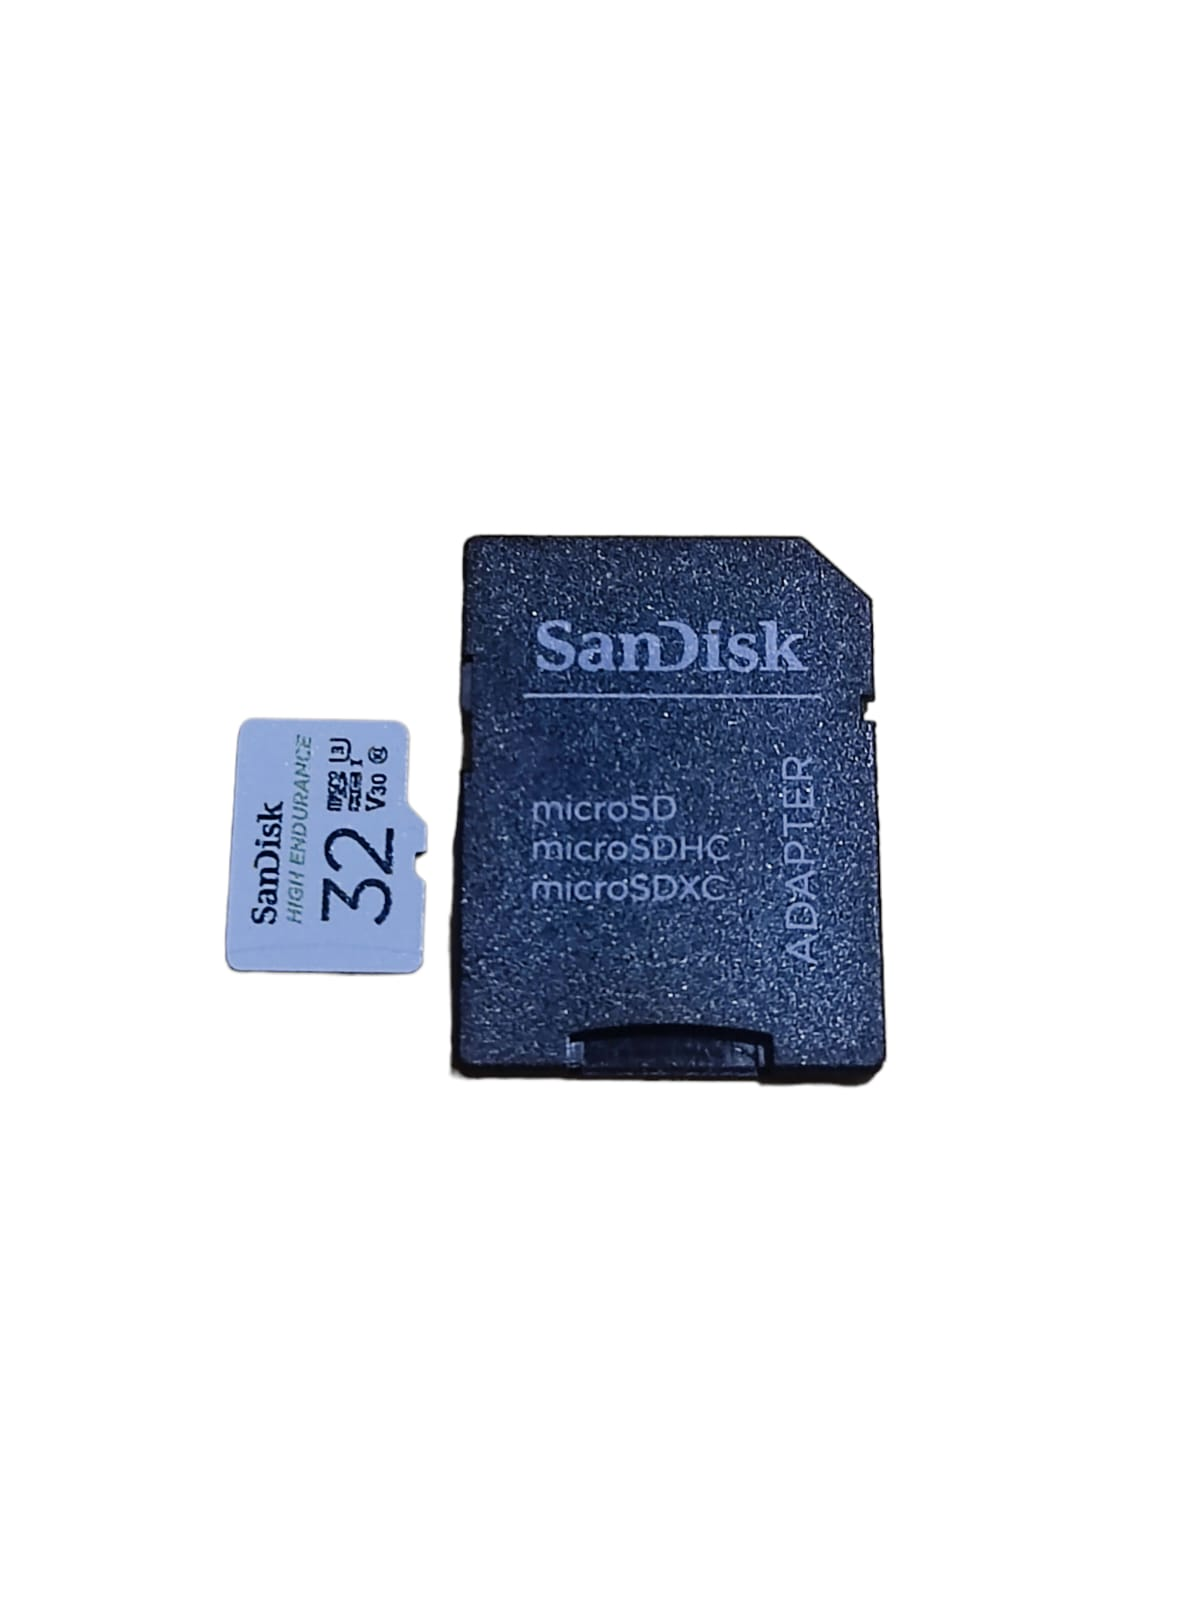
\includegraphics[width=0.35\linewidth]{document/figures/04_microSD_propia.jpg}
    \caption{MicroSD Sandisk High Endurance.  Fotografía, autoría propia}
    \label{fig:microsd}
\end{figure}

    \item \textbf{MS5611-01BA03}:  es un sensor de presión barométrica de alta precisión con un rango de operación de 10 a 1200 hPa acorde con gráfica de figura \ref{fig:atmosferica_tiempo} y \ref{fig:atmosferica_altitud},  ampliamente utilizado en aplicaciones que requieren mediciones exactas de altitud y control de altitud en dispositivos como drones, aviones y estaciones meteorológicas. Este sensor fue utilizado en estos trabajos \cite{pycubed, TASEC_Lab, navio_componentes}. En figura \ref{fig:MS5611} se muestra el dispositivo.

\begin{figure}[h]
    \centering
    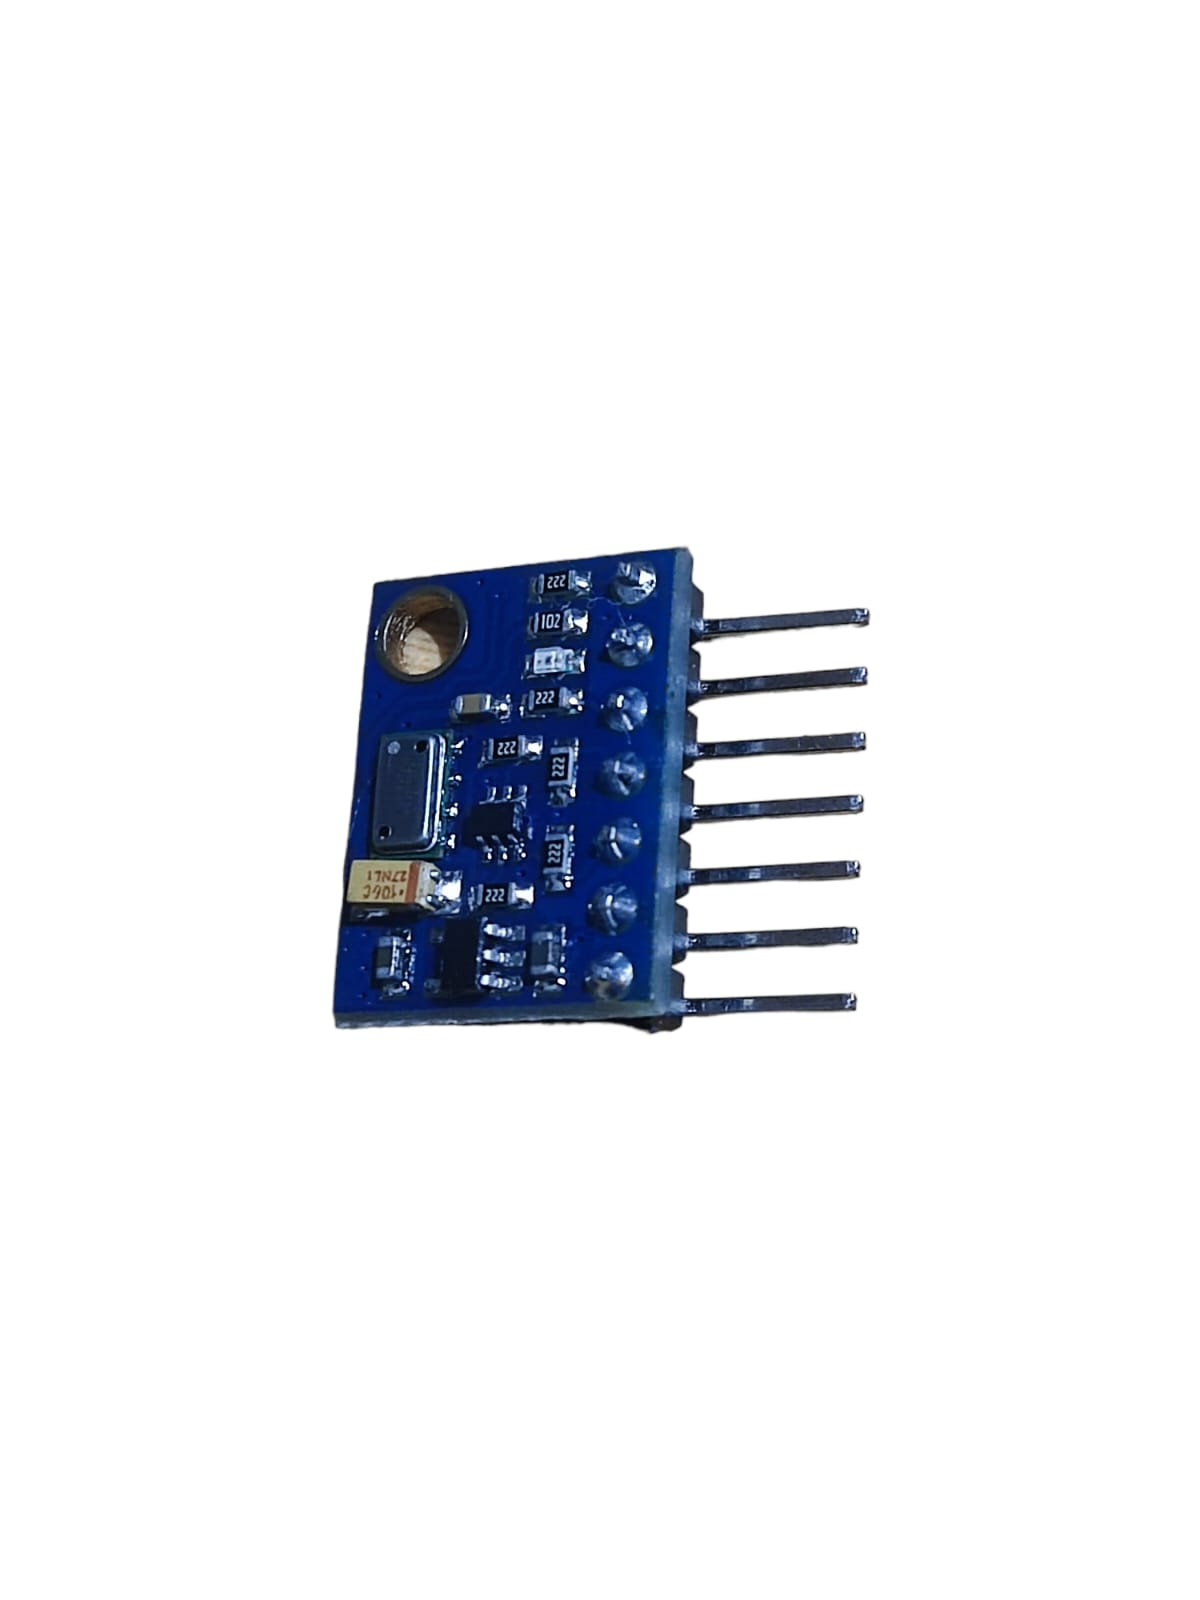
\includegraphics[width=0.25\linewidth]{document/figures/04_MS5611-01BA03_propia.jpg}
    \caption{Módulo genérico MS5611-01BA03.  Fotografía, autoría propia}
    \label{fig:MS5611}
\end{figure}

    \item \textbf{LSM9DS1:} la  se utiliza como IMU (inertial measurement unit) obedece a tener información del movimiento con su dirección y orientación del globo sonda, este IMU cuenta con 9 grados de libertad contando con un acelerómetro, magnetómetro y giroscópico de tres ejes todos respectivamente. Este sensor fue utilizado en estos trabajos \cite{pycubed, TASEC_Lab, navio_componentes}, además es ampliamente utilizado como complemento de GNSS para aumentar su precisión \cite{gnss}. En figura \ref{fig:imu} se muestra el equipo.

\begin{figure} [h]
    \centering
    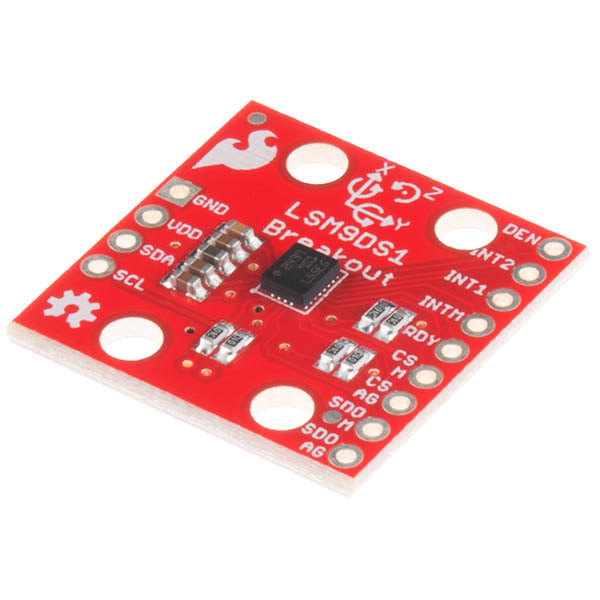
\includegraphics[width=0.25\linewidth]{document/figures/04_LSM9DS1_sparkfun.jpg}
    \caption{LSM9DS1, Créditos a SparkFun CC BY 2.0,  sin edición}
    \label{fig:imu}
\end{figure}

    \item \textbf{PT1000:}   los detectores de temperatura de resistencia (RTD) son sensores de temperatura que contienen una resistencia que cambia el valor de resistencia a medida que cambia su temperatura, la resistencia es en realidad una pequeña tira de platino con una resistencia de 1000 ohmios a 0 °C, de ahí el nombre PT1000. En comparación con la mayoría de los termistores NTC/PTC, el tipo PT de RTD es mucho más estable y preciso. En TASEC-Lab fueron utilizados para la caracterización dinámica del vuelo, así como también para conocer la convección de la atmosfera durante su experimento \cite{TASEC_Lab}. Se le adicionó un amplificador llamado MAX3186 desarrollado por Adafruit con el objetivo de facilitar el desarrollo, en figura \ref{fig:pt100+max} se aprecian ambos elementos. 

\begin{figure}[h]
    \centering
    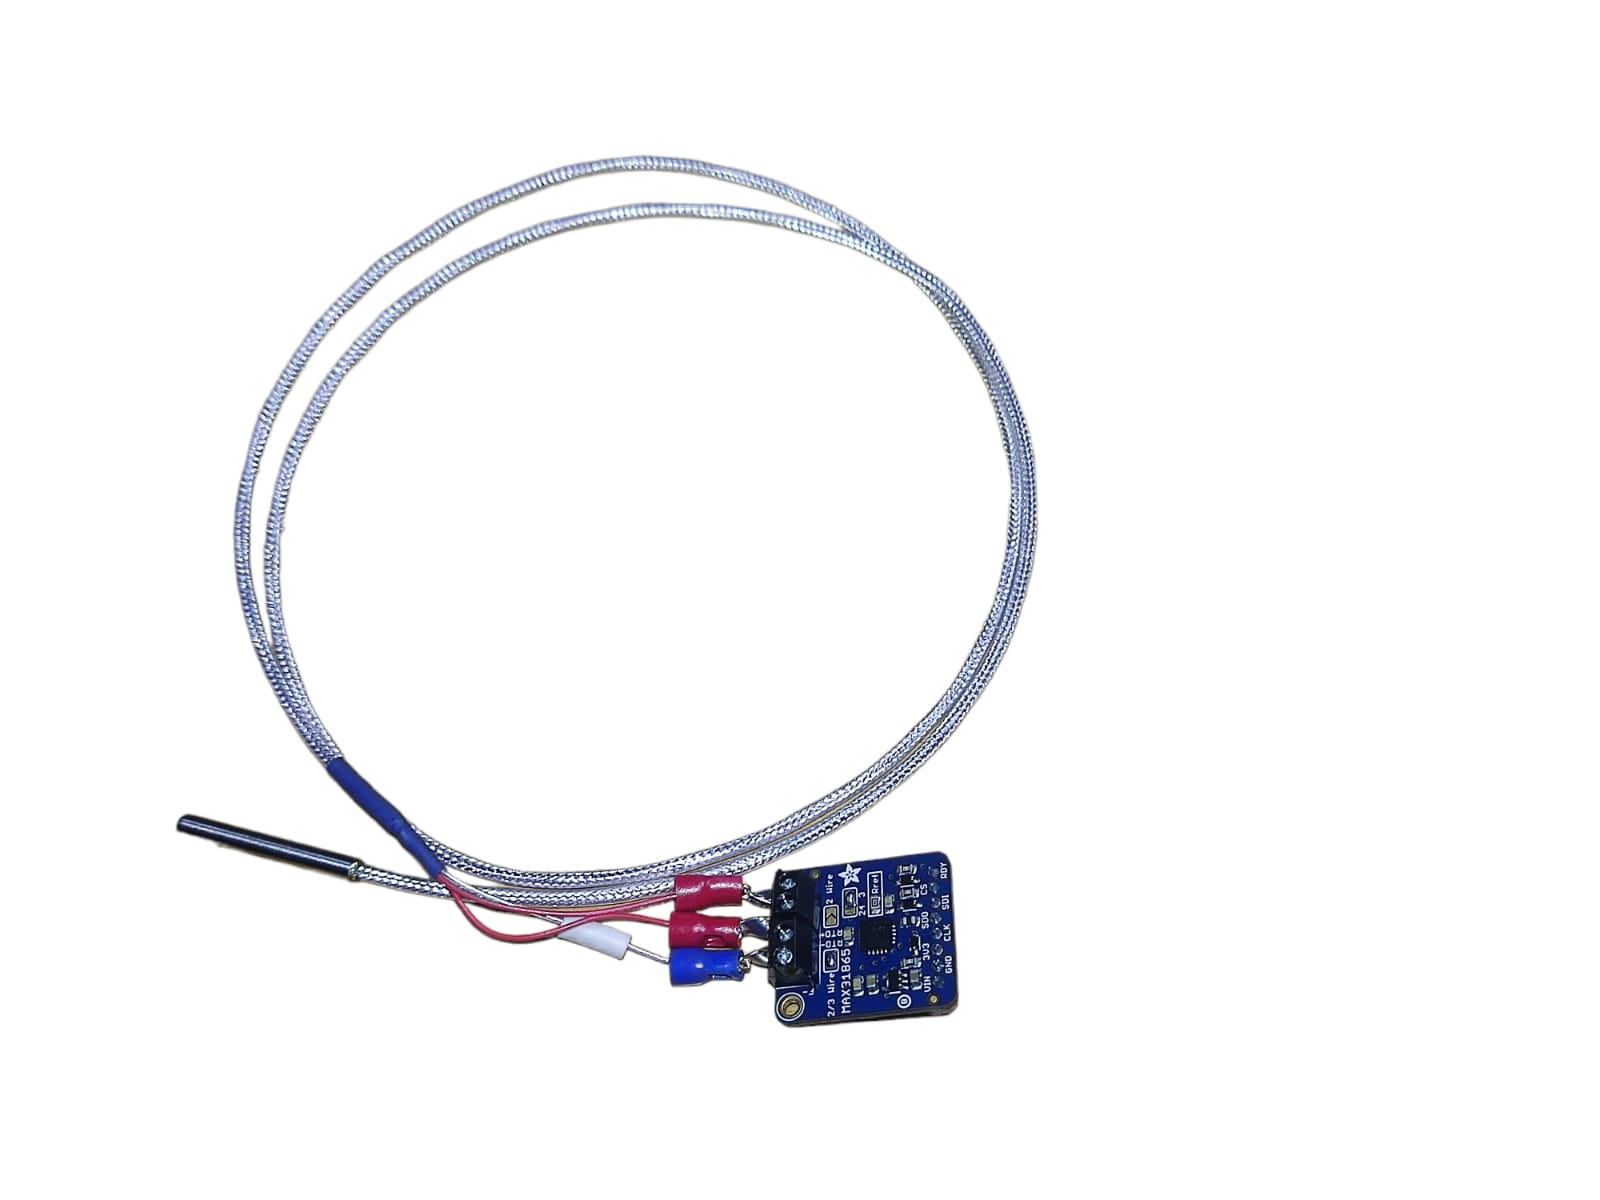
\includegraphics[width=0.5\linewidth]{document/figures/04_PT1000+MAX_propia.jpg}
   \caption{PT1000 junto con MAX31865 RTD. Fotografía, autoría propia}
    \label{fig:pt100+max}
\end{figure}

\item \textbf{Computadora a abordo:}  Es la unidad de procesamiento, responsable de recibir y procesar los datos E/S  provenientes de los diferentes  componentes con anterioridad mencionados. Se plateó utilizar  Arduino Nano V3 o SMT32 NUCLEO-L432KC debido se pueden intercambiar porque poseen el mismo socket (conector), las hojas técnicas mostró  que el STM32 posee características de duplicar en casi todo al Arduino, además posee un IDE con mejor integridad y mayor configurabilidad y más avanzado.   En figura \ref{fig:micro}, se muestra un Arduino Nano de forma ilustrativa para mostrar el socket.

\begin{figure}[h]
    \centering
    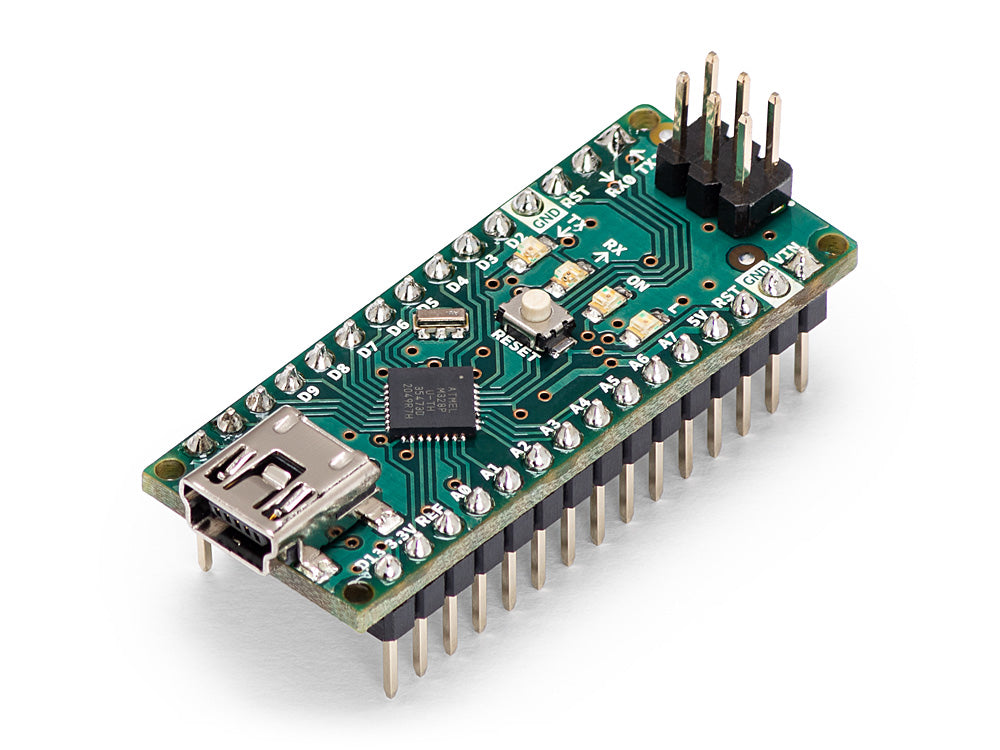
\includegraphics[width=0.25\linewidth]{document/figures/04_arduino_nano_v3.jpg}
    \caption{Arduino Nano Rev3.  Créditos a Arduino CC, CC BY-SA 4.0}
    \label{fig:micro}
\end{figure}

\end{itemize}

\vspace{0.5cm}

Todos los elementos mostrados son adecuados para la operación del globo sonda en las condiciones de temperatura y presión simuladas. Se seleccionaron componentes con alta documentación y pruebas en misiones similares y ninguno de los elementos mencionados es inflexible a cambios,  se buscó aproximar el mejor dimensionamiento. Se recomienda revisar los anexos para obtener información detallada sobre peso, consumo energético, dimensiones 3D y documentación específica de cada componente.

\newpage

\section{Dimensionamiento de Subsistema de Navegación}

Las dimensiones físicas de la PCB (Printed Circuit Board) se decide que son 12x8 cm y los componentes no mayores de 2.4 cm de altura, ya que esta es la división de los niveles entre cada subsistema, retomándose del trabajo anterior desarrollado en le marco StratoBalloon \cite{tesis_estructura_stratoballoon}. En el presente subsistema de navegación, por la selección realizada en los componentes, se  tienen conjunto de \textit{"módulos de placas de circuitos"} montados sobre una placa madre, siendo así que el diseño de los circuitos se ha aprovechado de la técnica de prototipado rápido y modular, lo cual permite agilizar el proceso de desarrollo.

\begin{figure}[h]
    \centering
    \includegraphics[width=0.95\linewidth]{document/figures/04_ckto_navegación.png}
    \caption{Diagrama de bloques del dimensionamiento.}
    \label{fig:diagrama_dimensionamiento}
\end{figure}

En la figura \ref{fig:diagrama_dimensionamiento} se presentan las conexiones. En el subsistema de navegación, se intentó que todos componentes internos tuvieran una conexión I2C  por la alta versatilidad que estos ofrecen, ejemplo de ello es el sistema de conexión Qwicc desarrollado por SparkFun \cite{qwiic}.  El registro de vuelo y sensor de temperatura debido a que solamente los protocolos UART y SPI  poseían respectivamente fueron los únicos con los que no se trabajó con I2C Por otro lado, los demás subsistemas (telemetría y energía) se proyecta que tengan una comunicación entre sus computadoras abordo con el protocolo I2C, sin embargo, en el marco StratoBalloon estos detalles pueden cambiar según necesidades de diseño y planeación.

\newpage

En este dimensionamiento, se ha omitido abordar aspectos más específicos relacionados con los subsistemas como telemetría y energía y solamente se consideró su comunicación y alimentación recibida por ellos,  sin embargo,  recuérdese que se trata de un proyecto que debe articularse con las diferentes partes involucradas (ver figura \ref{fig:diagrama_dimensionamiento}) y es necesario desarrollar pruebas de funcionamiento del mismo tanto en condiciones de simulación como en funcionalidad de software y hardware;  dejándose aquí establecido lo más adecuado con las características necesarias para asegurar el funcionamiento más óptimo posible de un subsistema de navegación y teniendo en cuenta los requisitos y las limitaciones de la misión con la simulación de trayectoria. Dicho lo anterior, se procede mostrar la disposición de los conjuntos de \textit{"módulos de placas de circuitos"} montados sobre una placa madre, como se muestra en figura \ref{fig:layout}, diseño de placa desarrollado en Fusion360.

\begin{figure} [h]
    \centering
    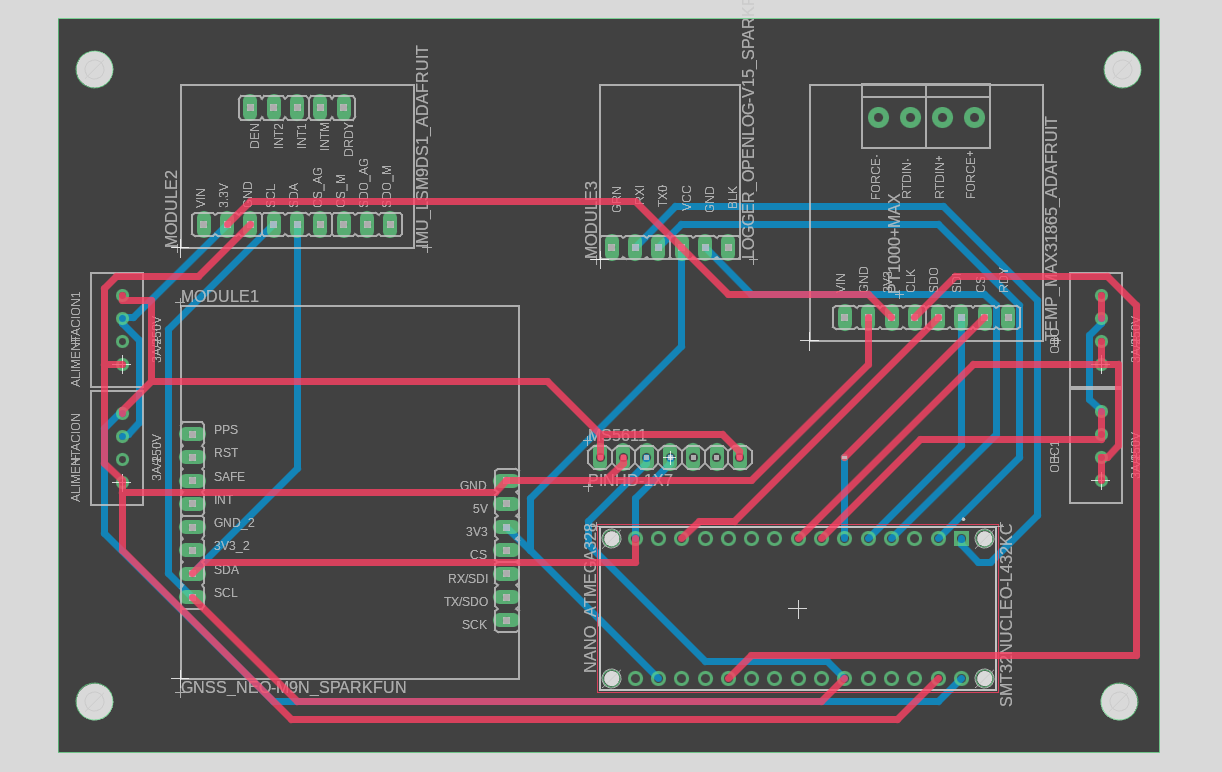
\includegraphics[width=0.75\linewidth]{document/figures/04_layout.png}
    \caption{Disposición de las pistas de la PCB, layout. }
    \label{fig:layout}
\end{figure}

El diseño es muy preliminar y puede estar sujetos a cambios, sin embargo, se tomaron ciertas consideraciones al momento de diseñar lo mostrado en figura \ref{fig:layout}:
\begin{itemize}
    \item Los laterales cortos (8 cm) de la placa son utilizados para la alimentación de energía y comunicación  con las diferentes placas que se proyectaron \cite{tesis_estructura_stratoballoon}.
    \item Todos los agujeros en los bordes de la placa tienen una dimensión de 4 mm de diámetro, útiles para facilitar el montaje y la fijación en la posible estructura de referencia \cite{tesis_estructura_stratoballoon}; y con respecto a la ubicación de cada agujero, están a una distancia de 5.5 mm con respecto al lateral de 8 cm y 4 mm con respecto al lateral de 12 cm, véase figura \ref{fig:agujeros_placa} amplía más esta idea y se puede consultar demás detalles en anexos \ref{chp:anexo:source_thesis}.

    \item Los conectores usados tanto para alimentación como para comunicación son JST B4B-XH-A, se usan por su alta versatilidad y disponibilidad en el mercado.
\end{itemize}

Con las anteriores consideraciones listadas, no se tomaron más consideraciones ni se siguieron estándares debido a lo complejo que pueden llegar hacer para una industria aeroespacial tan exigente, como también que este dimensionamiento es una tecnología introductoria que se espera que seguía desarrollando en el marco de StratoBalloon. Ejemplos de estándar podría ser PC104\footnote{Más información en la página oficia, es un estándar muy usual en nanosatélites. Link: \url{https://pc104.org/pc104-consortium/}} o consideraciones como distribución del calor o convección de los subsistemas a partir de simulaciones más complejas.  

\begin{figure}[h]
    \centering
    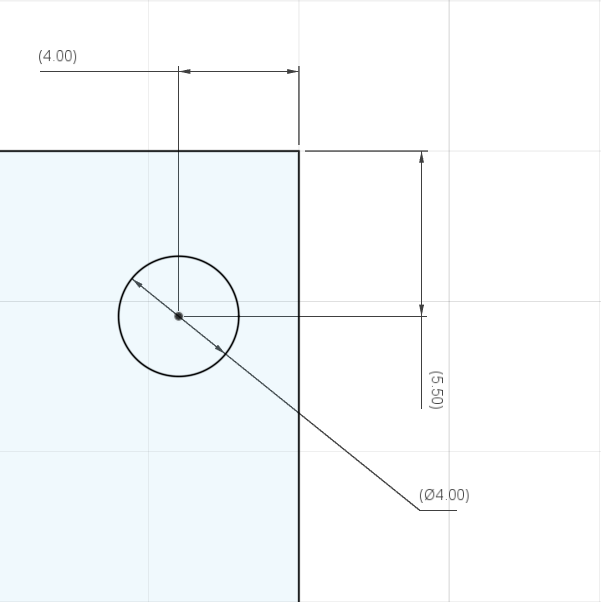
\includegraphics[width=0.75\linewidth]{document/figures/04_disposicion_agujero_PCB.png}
    \caption{Disposición de los agujeros en placa}
    \label{fig:agujeros_placa}
\end{figure}
\newpage
\begin{figure}[h]
    \centering
    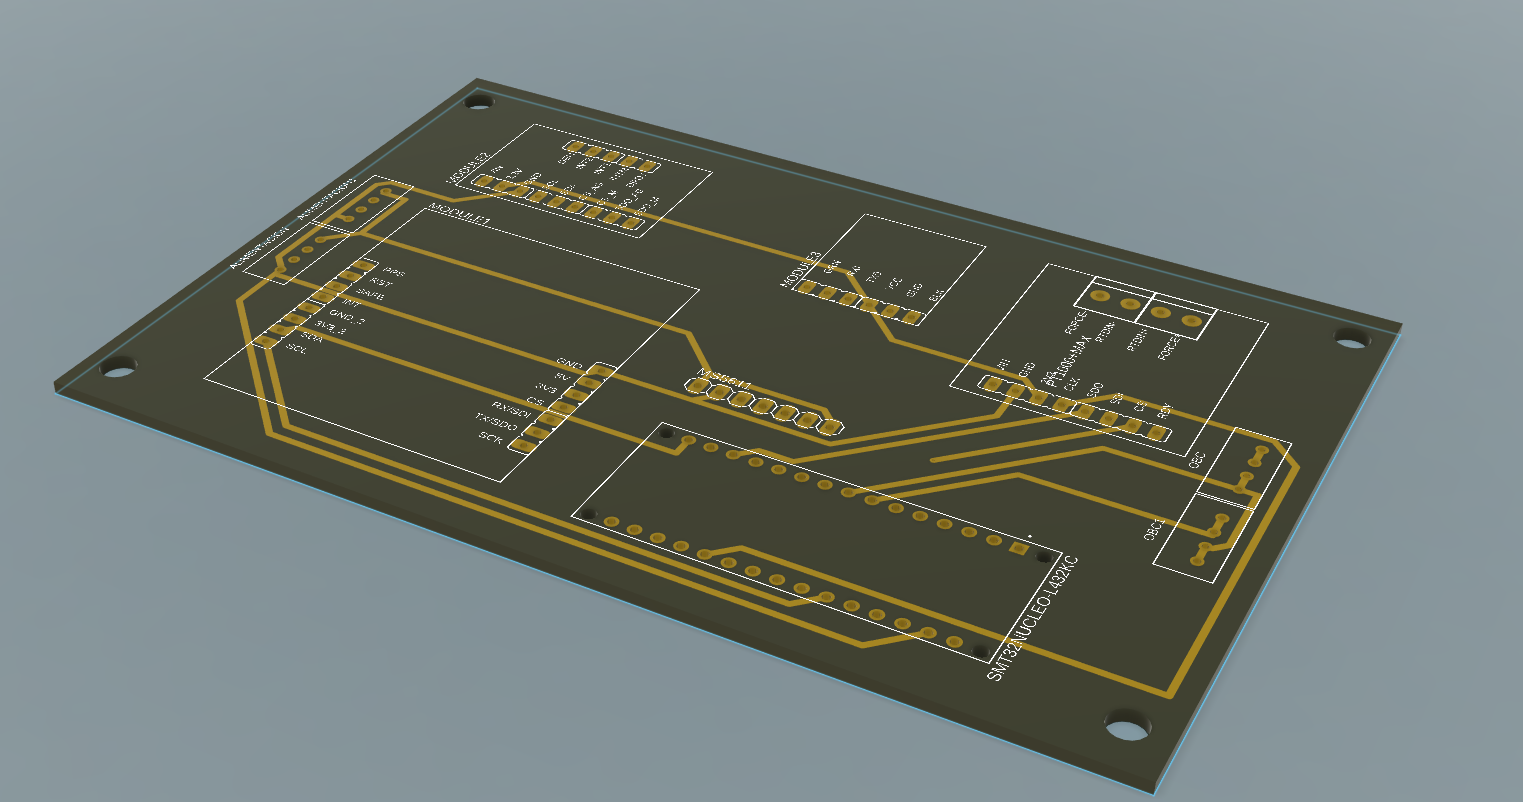
\includegraphics[width=1\linewidth]{document/figures/04_PCB v1_3D.png}
    \caption{Placa de Circuito en 3D.}
    \label{fig:PCB_3D}
\end{figure}

La figura \ref{fig:PCB_3D} muestra una representación en tres dimensiones de una placa que está lista para ser utilizada en prototipos y pruebas. El propósito de estas pruebas es evaluar la funcionalidad de cada componente dentro del contexto de la misión. La estrategia utilizada se basa en la idea de crear \textit{"módulos de placas de circuitos"} que serán ensamblados en una placa madre. Esta estrategia de diseño y ensamblaje se puede implementar en los laboratorios de la Universidad Don Bosco. Aunque en la fabricación actual no se usaron los archivos Gerber, estamos considerando generarlos para un posible proceso de manufactura futuro. Esto implica que el diseño actual podría ser adaptado y optimizado en una sola placa en caso de que se decida avanzar en la producción a lo largo de StratoBalloon. 

La manufactura en el extranjero, asumiéndose una optimización del diseño anterior de figura \ref{fig:PCB_3D},  se tiene que en cuanto a los parámetros de fabricación, se debe tener en cuenta el fabricante seleccionado y el tipo de material utilizado en la manufactura son factores determinantes. Se sugiere utilizar FR4 estándar para prototipos y FR408HR para la versión final de vuelo en futuras misiones; para el diseño con FR408HR, se especifica una impedancia controlada de 50 ohmios, con anchos de traza externos de 11 mils y anchos de traza internos de 10.7 mils según \cite{pycubed}.

\newpage

Es relevante destacar que la elección de los componentes electrónicos se llevó a cabo con base en hojas técnicas y datos ambientales adquiridos a través de simulaciones en capítulo \ref{chp:03_eda}. A pesar de que estos datos no replican directamente las condiciones reales de una misión, proporcionan una aproximación significativa que disminuye el riesgo al obtener información durante un vuelo en gloo estratosférico. Los detalles completos y respaldos de esta selección se encuentran en el anexo \ref{chp:anexo:componentes_analizados&extras}. En dicho anexo, se presentan tablas que muestran la temperatura de operación, la sensibilidad, el peso, el consumo y otros parámetros relevantes de los componentes. 

En anexo \ref{chp:anexo:pcb_layout_esquematico} se puede observar el diagrama esquemático y layout. Además, los archivos generados en este capítulo se pueden consultar con las indicaciones dadas en anexo \ref{chp:anexo:source_thesis}


% Finalización de Trabajo
\chapter{Recomendaciones y conclusiones} \label{chp:resultados}

\vspace{0.4cm}

Este capítulo marca el final de este trabajo de graduación. Aquí se presentan las conclusiones obtenidas a partir de esta investigación y se bridan recomendaciones para futuros proyectos de graduación que podrían derivarse de este estudio o ideas nuevas para futuros trabajos de graduación

\newpage

%%%%%%%%%%%%%%%%%%%%%%%%%%%%%%%%%%%%%%%%%%%%%%%%%%%%%%%%%%%%%%%%%%%%%%%%%%%%%%%%
%%%%%%%%%%%%%%%%%%%%%%%%%%%%%%%%%%%%%%%%%%%%%%%%%%%%%%%%%%%%%%%%%%%%%%%%%%%%%%%%


\section{Conclusiones} \label{sct:resultados_conclusiones}

Las misiones near-space representan una valiosa fuente para disciplinas STEM (science, technology, engineering y mathematics) debido a que generan pruebas de concepto reales; además,  representa una oportunidad para que países en vías de desarrollo como El Salvador se fomenten y avancen en carreras STEM y también aporta a los objetivos del desarrollo sostenible como \textit{Educación de Calidad}, \textit{Trabajo decente y desarrollo económico} e \textit{Industria, innovación e infraestructura}. A continuación, las conclusiones particulares: 

\begin{itemize}
    \item La visualización y análisis de datos desempeñaron un papel destacado al permitir comprender y detectar patrones y tendencias subyacentes en los datos simulados. A través de esta exploración detallada, se identificaron factores críticos que influyen en la trayectoria del globo sonda, siendo la presión y la temperatura los dos elementos más destacados de las variables analizadas. La presión, desempeña un papel fundamental en la integridad del globo, se reveló que varía de 1013.25 hPa (1 atm) sobre la superficie de la tierra a un mínimo de 12 hPa en la altitud objetivo de la misión de la simulación, siendo así puntos cruciales a considerar en futuras misiones. De igual manera, el control y monitoreo de la temperatura emerge para futuras misiones como elementos esenciales para garantizar un ascenso y descenso exitosos, debido a que existe una alta convección térmica que generará estrés al sistema y además la mayor parte de la misión se efectúa en temperaturas bajo cero oscilando de la temperatura ambiente a -56.6 °C. Además, la variación mínima en la gravedad a lo largo de la trayectoria del globo sonda plantea una importante implicación para qué se puede considerarse constante si se desea, ya que  su cambio fue a partir de la gravedad nominal a  la variación mínima del -0.93\% respecto a la nominal. La asimetría temporal en la duración de la misión, con un 75\% del tiempo total dedicado al ascenso y un 25\% al descenso, resalta la necesidad de considerar este tiempo en la planificación y un diseño específico para la recuperación de la sonda. Estos hallazgos, derivados del análisis de datos, proporcionan una base sólida para el diseño y la planificación de futuras misiones de globo sonda, mejorando significativamente la comprensión y capacidad de abordar los desafíos inherentes a este tipo de misones aeroespaciales.
    \item En el dimensionamiento del subsistema de navegación, se ha empleado un enfoque de prototipado rápido y modular, aprovechando las comunidades de hardware abierto. Es crucial resaltar que las consideraciones relacionadas con la atmósfera desempeñan un papel fundamental en la selección de componentes tecnológicos, ya que tanto la presión como la temperatura condicionan los requisitos de la misión.
\newpage
    \item  La simulación ha demostrado un rendimiento satisfactorio en la descripción de la trayectoria del globo sonda, proporcionando condiciones relevantes para su desarrollo. Es esencial destacar que el simulador representa un paso inicial y está sujeto a ciertas limitaciones derivadas de las suposiciones realizadas. Además, el modelo se ve restringido por la disponibilidad de datos en tiempo real, ya que Python obtiene información del viento a través de la librería `getgfs`, basándose en datos de la NOAA y el modelo numérico GFS con una capacidad de consulta limitada hasta una semana en el pasado. Por otra parte, la selección de Python como nuestro lenguaje de programación, mostró su notable flexibilidad, portabilidad y accesibilidad, en comparación con los lenguajes académicos tradicionales como MATLAB. Es relevante mencionar que Python no requiere licencias, lo que lo convierte en una herramienta altamente conveniente para nuestros fines.
\end{itemize}

A pesar de ser un estudio preliminar con tecnología introductoria, se lograron alcanzar los objetivos establecidos, brindando una visión inicial de la temática estudiada. 


\newpage

%%%%%%%%%%%%%%%%%%%%%%%%%%%%%%%%%%%%%%%%%%%%%%%%%%%%%%%%%%%%%%%%%%%%%%%%%%%%%%%%
%%%%%%%%%%%%%%%%%%%%%%%%%%%%%%%%%%%%%%%%%%%%%%%%%%%%%%%%%%%%%%%%%%%%%%%%%%%%%%%%

\section{Trabajo futuro} \label{sct:resultados_trabajofuturo}

A continuación, se presentan sugerencias y recomendaciones que podrían considerarse en futuros trabajos, basadas en los hallazgos y limitaciones del presente estudio. A continuación, reflexionamos sobre estas recomendaciones:

\subsection{Simulador}

\begin{itemize}
    \item En el simulador se utilizó un modelo atmosférico simplificado, el modelo ISA, y se asumió un día aleatorio que involucraba un acontecimiento típico de la sonda en su trayectoria y  a partir de esta asunción se hizo un dimensionamiento del subsistema de navegación el cual se tiene que complementar con medidas de protección y estructurales. Sin embargo, para obtener datos más realistas, se sugiere desarrollar simulaciones en diversos escenarios y condiciones climáticas utilizando datos proporcionados por la NOAA a través de su modelo GFS, incluyendo información sobre humedad, vientos,  presión y temperatura, además de corregir la implementación de los vientos en el simulador. Esta conexión con la NOAA está respaldada por una amplia documentación que válida su factibilidad en el desarrollo \cite{grid_python, consumo_datos_NOAA, info_acceso_NOAA, explicacion_consumo_datos_NOAA} y  el tratamiento de los datos se soluciona haciendo una interpolación multivariable, tal como se hizo en este trabajo haciendo un paralelepípedo con interpolación múltiple y multivariable \cite{spain_simulador}.  Luego de todo lo anterior,  se debe de hacer un análisis temporal con un simulador más completo y datos más realistas. Además, se puede desarrollar una interfaz gráfica de usuario para facilitar la utilización del simulador, brindando mayor accesibilidad y una experiencia más amigable.

    \item El simulador debe hacer cálculos de peso que podrá soportar automáticamente, para efectos prácticos, acá en esta simulación se hizo con un peso de antemano, sé sabia que existía flotabilidad. Además, los cálculos se podría hacer aún más realistas considerando 6 grados de libertad y una matriz inercial para el sistema,  y así, se deja de lado el punto de masa con tres grados de libertad desarrollado en este trabajo.

    \item Comparar datos del simulador con datos reales de vuelo mejora la descripción de la trayectoria. Esto permite agregar nuevos modelos al simulador, aumentando la precisión, como se menciona en las referencias y se hace en \cite{simulador_chino, parachute_6DOF, paracaidas_simplificado_futuro}. 

\end{itemize}

\newpage

A continuación se presenta un resumen de las variables utilizadas para ser punto de partida para otros trabajos:


\begin{enumerate}
    \item \textbf{Tiempo (\(t\)):} Unidad de sucesos que describe la trayectoria de ascenso y descenso.
    
    \item \textbf{Posición Geográfica:}
    \begin{itemize}
        \item \textbf{Latitud (\(\phi\)):} Coordenada norte-sur donde se ubica la sonda en la superficie de la Tierra.
        \item \textbf{Longitud (\(\lambda\)):} Coordenada este-oeste donde se ubica la sonda en la superficie de la Tierra.
        \item \textbf{Altitud (\(z\)):} Elevación vertical sobre la superficie de la Tierra donde se ubica la sonda.
    \end{itemize}
    
    \item \textbf{Velocidades:}
    \begin{itemize}
        \item \textbf{Velocidad Vertical (\(\frac{dz}{dt}\)):} Cambio de posición vertical de la sonda por unidad de tiempo.
        \item \textbf{Velocidad del Viento \(U\):} Componente de viento paralela a la latitud (positiva de oeste a este).
        \item \textbf{Velocidad del Viento \(V\):} Componente de viento paralela a la longitud (positiva de sur a norte).
    \end{itemize}
    
    \item \textbf{Propiedades Atmosféricas:}
    \begin{itemize}
        \item \textbf{Temperatura:} Temperatura atmosférica basada en ISA a lo largo de la trayectoria.
        \item \textbf{Presión:} Presión atmosférica basada en ISA a lo largo de la trayectoria.
        \item \textbf{Densidad:} Densidad atmosférica a lo largo de la trayectoria, calculado con la temperatura y presión de la ISA.
        \item \textbf{Gravedad:} Intensidad del campo gravitatorio en función de la altitud.
    \end{itemize}
    
    \item \textbf{Dimensión del Globo:}
    \begin{itemize}
        \item \textbf{Diámetro del Globo:} Longitud transversal del globo utilizado.
    \end{itemize}
\end{enumerate}

\newpage

\subsection{Subsistema de Navegación}

\begin{itemize}
    \item Se recomienda realizar pruebas simulando las condiciones reales de la misión en los equipos tecnológicos para evaluar su funcionalidad. Posteriormente, se puede considerar enviar las tecnologías desarrolladas a fabricantes de PCB como Advanced Circuits, PCBWay y JLPCB, quienes ofrecen flexibilidad y personalización en la impresión de tarjetas.
    \item Es imprescindible analizar la integración con el resto de subsistemas electrónicos, considerando los protocolos de comunicación, el cableado de alimentación, interferencias y la seguridad operativa de las misiones.
\end{itemize}




%%%%%%%%%%%%%%%%%%%%%%%%%%%%%%%%%%%%%%%%%%%%%%%%%%%%%%%%%%%%%%%%%%%%%%%%%%%%%%%%
%%%%%%%%%%%%%%%%%%%%%%%%%%%%%%%%%%%%%%%%%%%%%%%%%%%%%%%%%%%%%%%%%%%%%%%%%%%%%%%%

% Documento de ayuda que explica los campos soportados por cada tipo de elemento en la bibliografía

% Referencias
\clearpage
\renewcommand{\bibfont}{\normalsize}
\printbibliography[heading=bibintoc, title={Referencias}]
% Glosario, acrónimos
% \clearpage
% \glsaddall
% \printglossary[type=\acronymtype]
% \printglossary

%   Nomenclarutas:
% \newpage
% % \section*{Nomenclature}

% % Configuración del espaciado de las nomemclaturas
% \renewcommand{\baselinestretch}{0.75}\normalsize
% \renewcommand{\aclabelfont}[1]{\textsc{\acsfont{#1}}}

%  % Comenzamos las nomenclaturas
% \begin{acronym}[longest]
%     \acro{t}[$t_{db}$]{dry-bulb air temperature\acroextra{, $^{\circ}$C}}
%     \acro{t-w}[$t_{wb}$]{wet-bulb air temperature\acroextra{, $^{\circ}$C}}
%     \acro{rh}[RH]{relative humidity}
%     \acro{c}[$c$]{speed of light in a vacuum inertial system} 
% \end{acronym}
% \renewcommand{\baselinestretch}{1}\normalsize

%% Anexos
\frontmatter % Numeración  romana de aquí en adelante:
\appendix
\clearpage
%\addcontentsline{toc}{chapter}{\annexname}
\chapter{Anexo} \label{chp:anexo}

\section{Conceptos Básicos}

\subsection{Hidrostática} \label{chp:anexo:hidrostatica}

Para representar las propiedades de un fluido en reposo, como la presión, en función de la altura y la densidad, se utiliza comúnmente la ecuación de la hidrostática, que es una aproximación matemática que se aplica a fluidos en condiciones normales de temperatura y presión.

La ecuación de la hidrostática establece que la presión, la altura, la densidad y la aceleración gravitacional del fluido están relacionados \cite{libro_fisica_giancoli}, mediante la siguiente fórmula:

\begin{equation}
    \label{eq:hidrostatica}
    P=\rho gh 
\end{equation}

Donde en ecuación \ref{eq:hidrostatica}:

\begin{itemize}
    \item $P$ es la presión del fluido (en Pascales)
    \item $\rho$ es la densidad del fluido en $kg/m^{3}$   
    \item $g$ es la aceleración gravitacional (en $m/s^{2}$
    \item $h$ es la altura del fluido (en metros)
\end{itemize}

\newpage

\subsection{Gases Ideales} \label{chp:anexo:gases_ideales}

Para representar las propiedades de un gas, como la densidad, en función de la temperatura y la presión, se utiliza comúnmente la ecuación de estado del gas ideal, que es una aproximación matemática que se aplica a gases en condiciones normales de temperatura y presión.

La ecuación de estado del gas ideal establece que la presión, el volumen, la cantidad de sustancia y la temperatura de un gas están relacionados \cite{libro_fisica_giancoli}, mediante la siguiente fórmula:

\begin{equation}
    \label{eq:gasesideales}
    PV = nRT 
\end{equation}


Donde en ecuación \ref{eq:gasesideales}:

\begin{itemize}
    \item $P$ es la presión del gas (en Pascales)
    \item  $V$ es el volumen ocupado por el gas (en metros cúbicos)
    \item  $n$ es la cantidad de sustancia del gas (en moles)
    \item  $R$ es la constante de los gases ideales (8,31 J/mol*K)
    \item  $T$ es la temperatura del gas (en Kelvin)
\end{itemize}


\newpage

\section{Componentes analizados para subsistema de Navegación} \label{chp:anexo:componentes_analizados&extras}

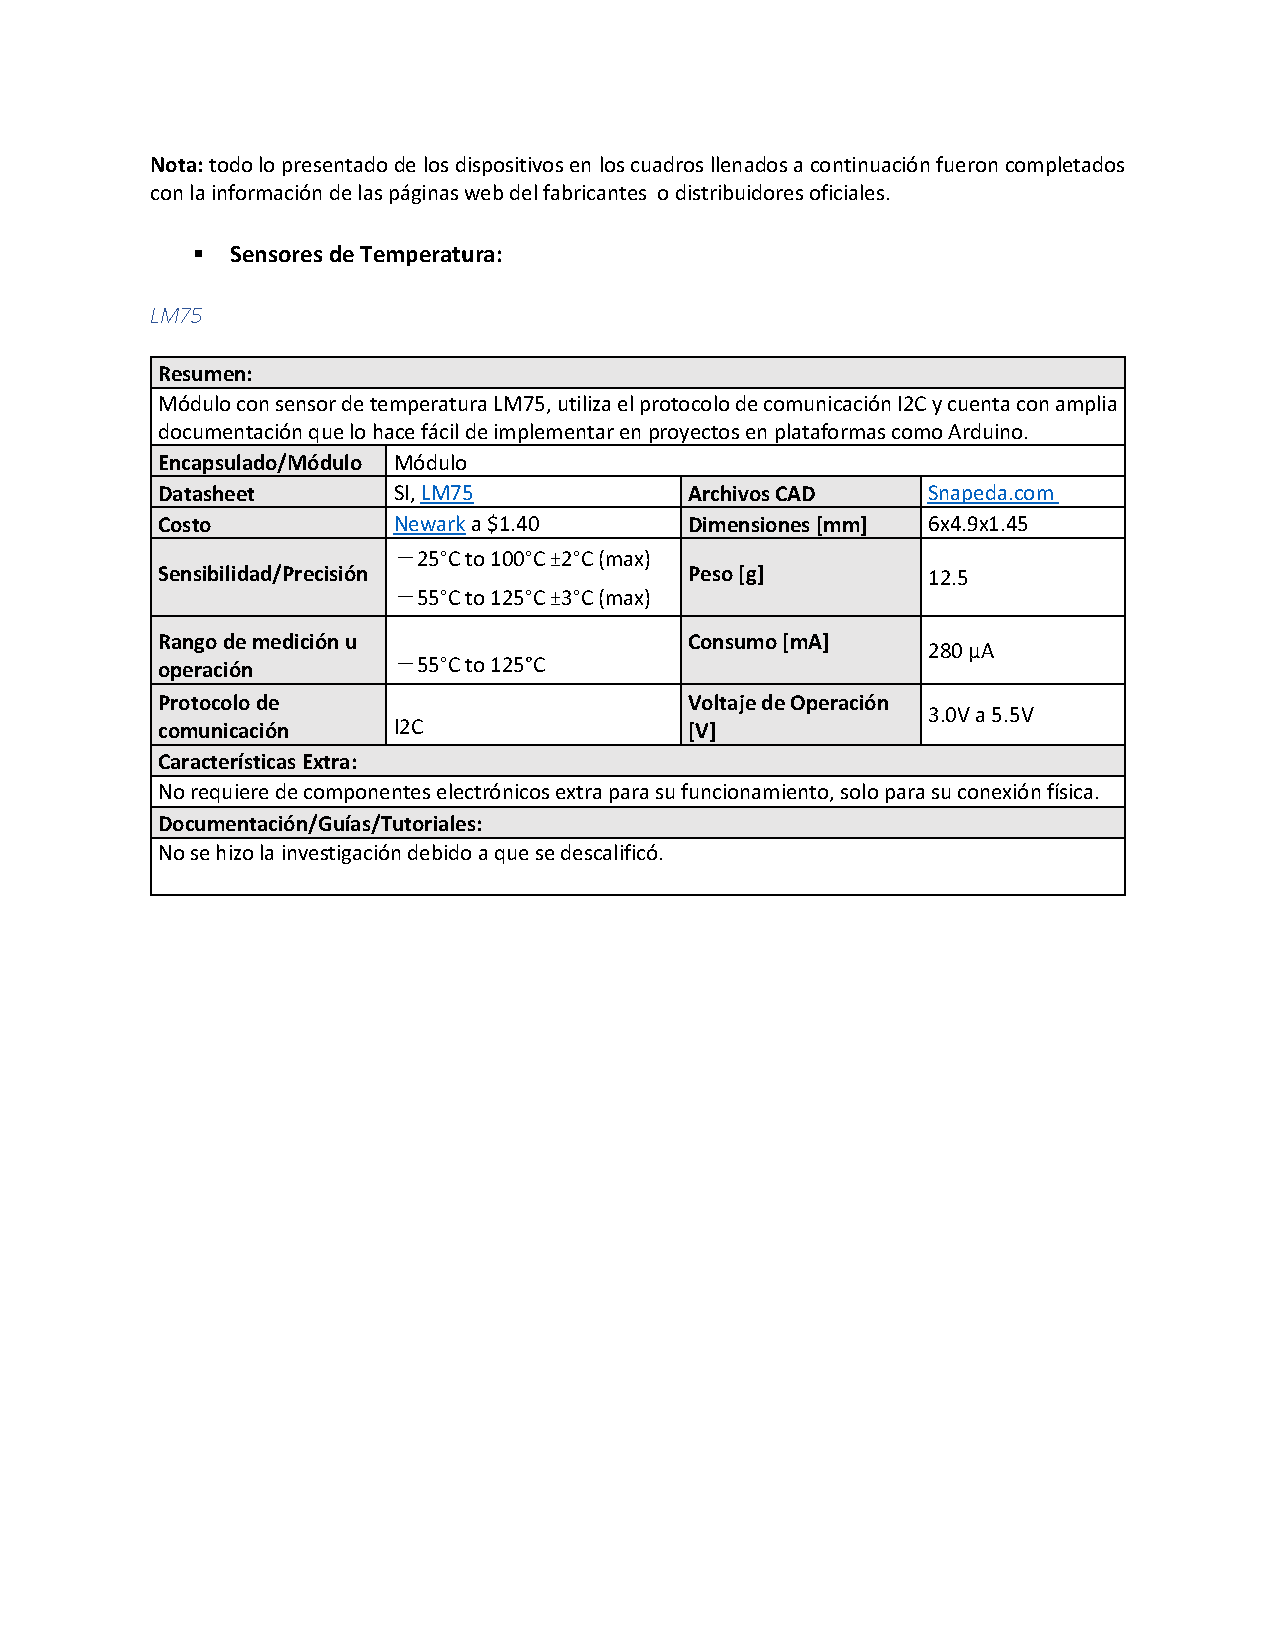
\includepdf[pages=-, scale=1]{document/annexes/seleccion_hardware.pdf}


\section{Diseño de Placa de Circuito para dimensionamiento de Subsistema de Navegación} \label{chp:anexo:pcb_layout_esquematico}

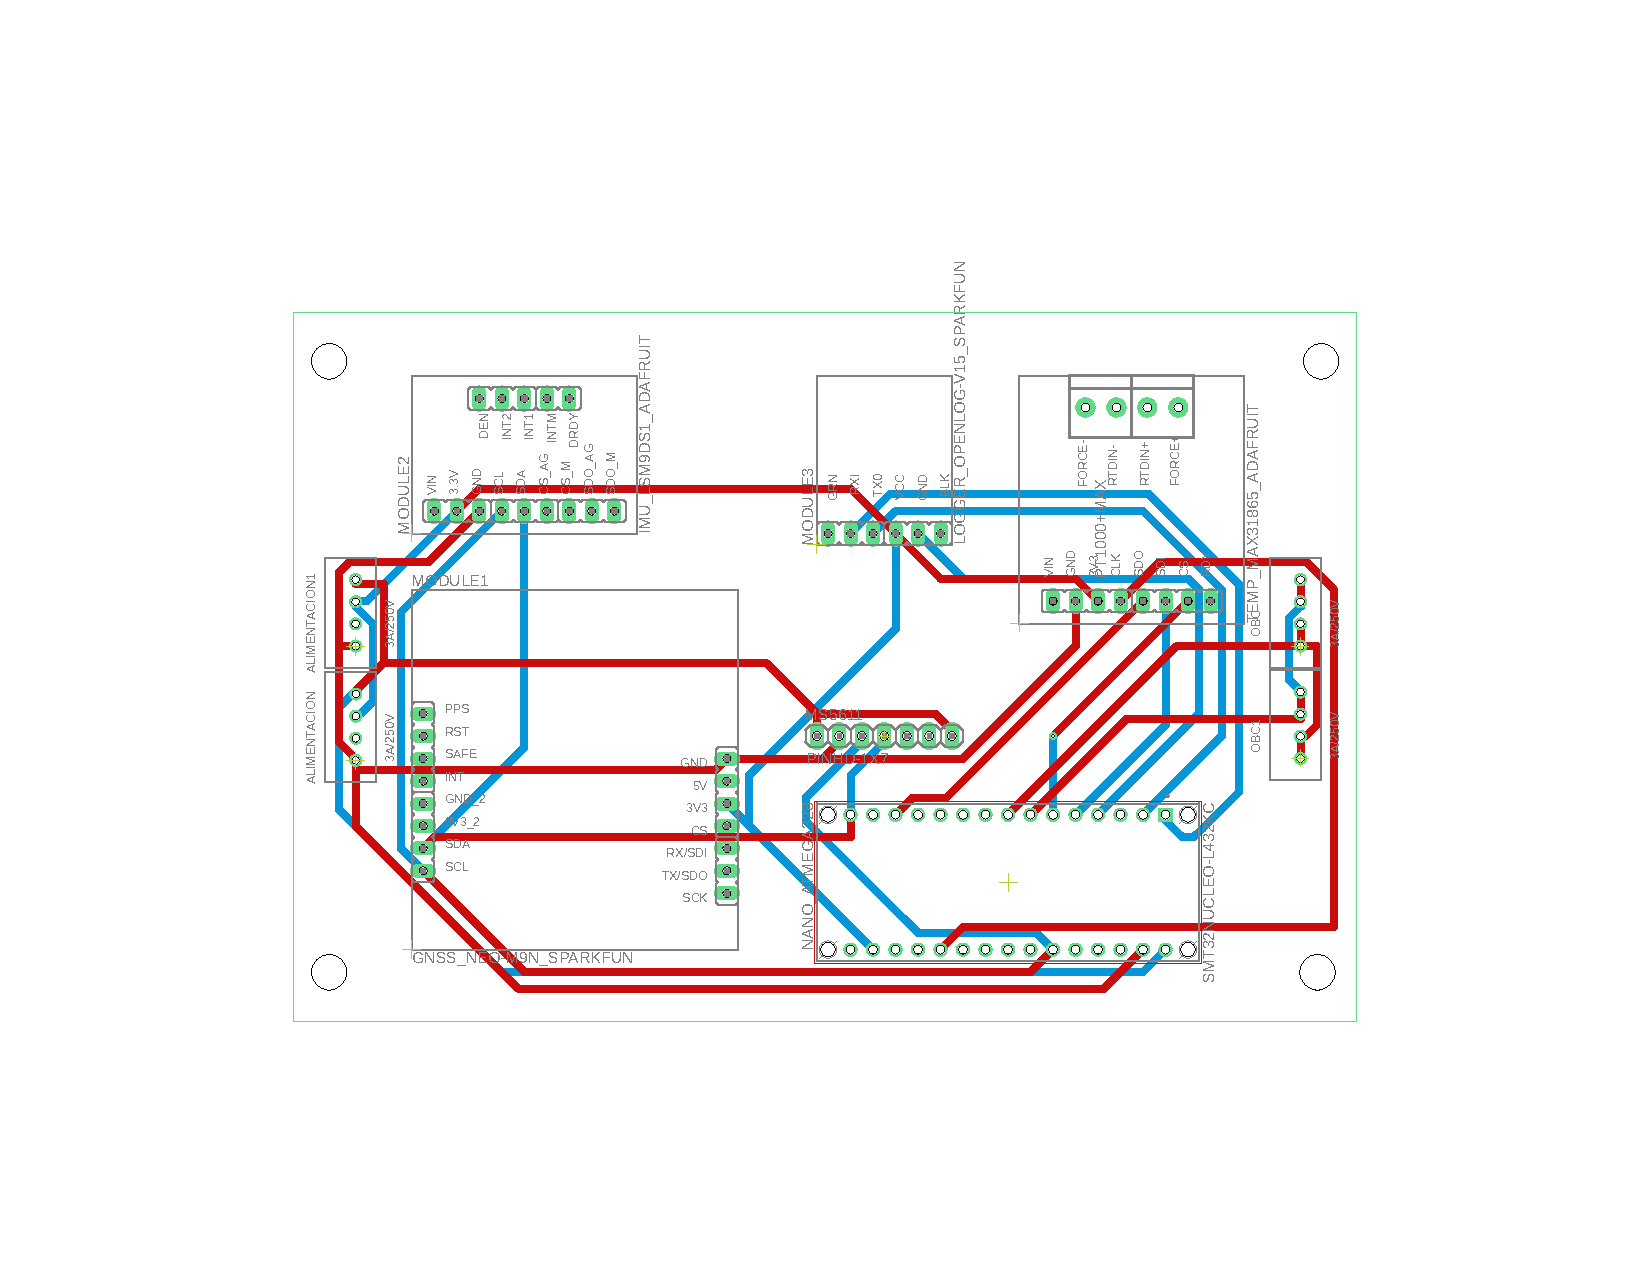
\includepdf[pages=-, angle=90]{document/annexes/PCB_layout.pdf}

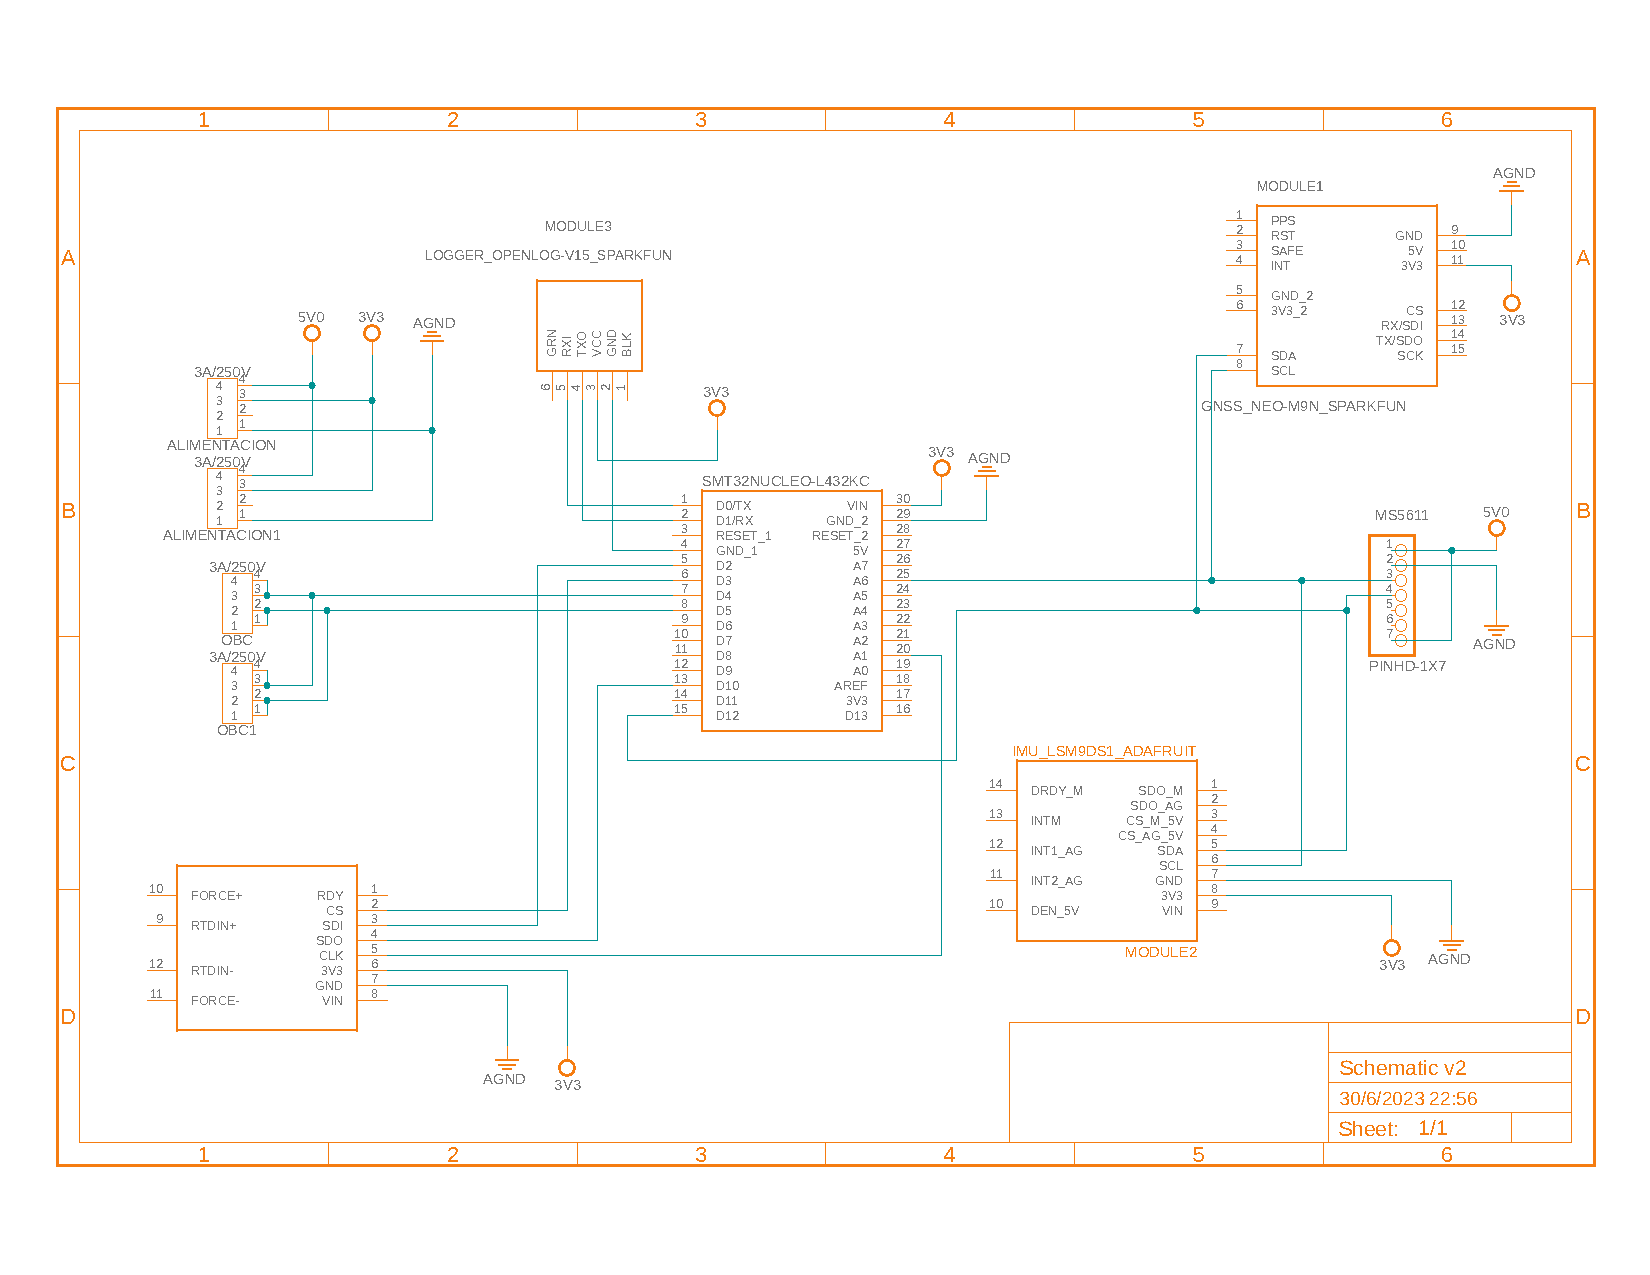
\includepdf[pages=-, angle=90, scale=0.8]{document/annexes/esquematico.pdf}

\newpage

\section{Recursos y herramientas}  \label{chp:anexo:source_thesis}

\begin{flushleft}
{\sffamily\small\textit{Las herramientas utilizadas fueron: }}

\begin{itemize}
    \item {\sffamily\bfseries\small\textit{\LaTeX     \space fue utilizado como editor de texto. Utilizando Overleaf.}}
    \item {\sffamily\bfseries\small\textit{Python junto con Jupyter Notebooks fue utilizado como herramienta de programación.  }}
\end{itemize}

\vspace{1cm}

{\sffamily\bfseries\small\textit{El código fuente y todo lo realizado en la presente fue cargado en un repositorio Online llamado GitHub, el repositorio online se puede visitar en el siguiente enlace: }}

\vspace{0.5cm}

\begin{center}
\href{https://github.com/osminlab/Proyec_Gda_Simula_PCB_Nav}{https://github.com/osminlab/Proyec\_Gda\_Simula\_PCB\_Nav}
\end{center} 

\vspace{0.5cm}

\textbf{Nota 1: } {\sffamily\small\textit{En el repositorio de GitHub se encuentran  muchos archivos README.md que guía y explican como está distribuido toda la información perteneciente a este trabajo de graduación.}}

\textbf{Nota 2:} {\sffamily\small\textit{Todas las imágenes son de autoría personal a menos que se diga lo contrario. Algunas imágenes son de búsqueda en Google con el filtro de 'Creative Commons licenses',  o de autores específicos que se han dado sus créditos respectivos en este trabajo. Además, se crea una carpeta llamada 'LICENSES' en el repositorio por todas las imágenes tomadas de tercero.}}
\end{flushleft}



%%-----------------------------------------------






\end{document}
